%\documentclass[red, hyperref={pdfpagelabels=false}]{beamer}
\documentclass[red]{beamer}
\hypersetup{pdfpagemode=FullScreen}

\mode<presentation>
\usepackage{beamerthemesplit}
\usepackage[T1]{fontenc}
\usepackage{textcomp}
\usepackage{lmodern}
\usepackage{siunitx}
%\usepackage{listings,bera}
%\usepackage{color}

%\usetheme{boxes}
%\usetheme{Darmstadt}
\usetheme{Dresden}
%\usetheme{Frankfurt}
%\usetheme{Ilmenau}
%\usetheme{Madrid}
%\usetheme{Warsaw}
\beamertemplatenavigationsymbolsempty

\title{Estimating and Mitigating Errors in Dual-Polarization Radar Attenuation Correction}
\author{Ryan May}
\date{08 September 2014}
\titlegraphic{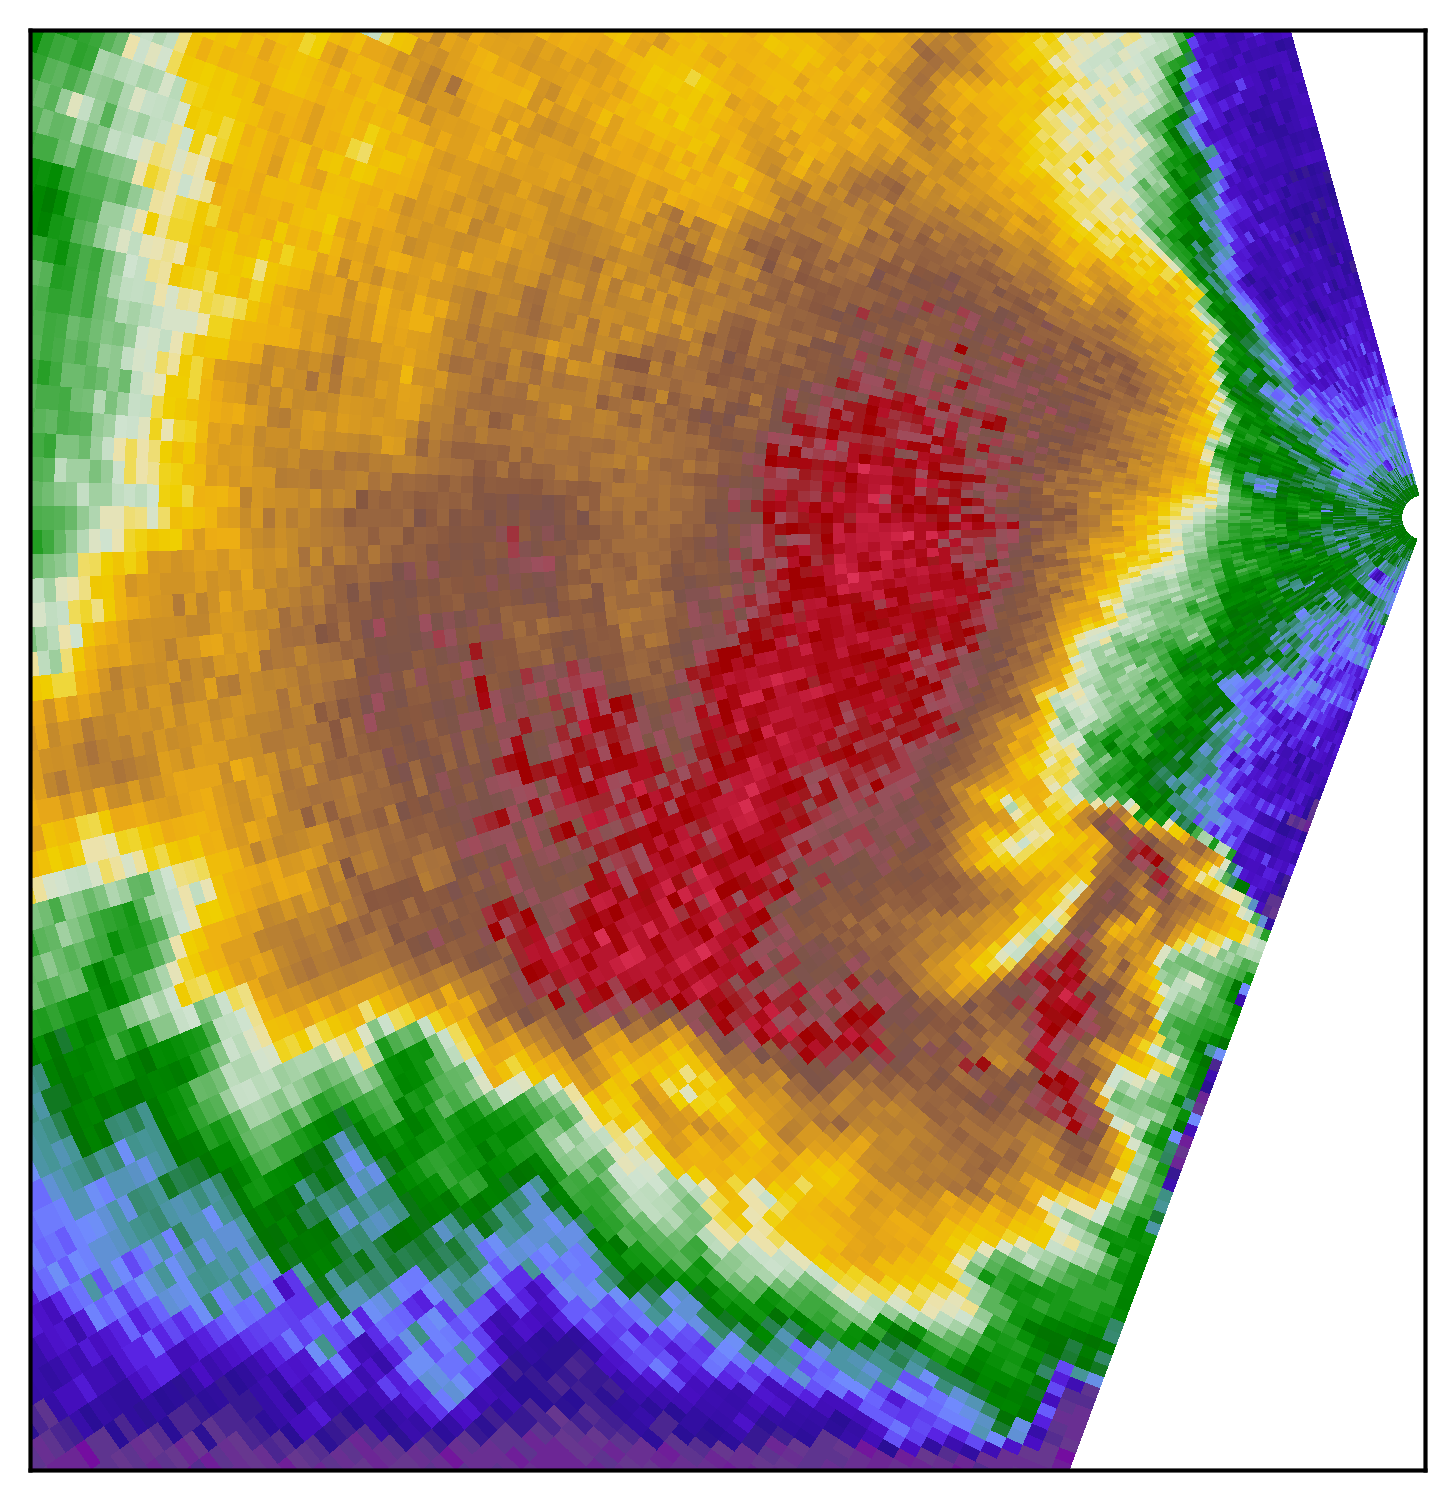
\includegraphics[scale=0.17]{figures/title_ppi.png}}

\begin{document}

\begin{frame}
	\titlepage
\end{frame}

\begin{frame}{Outline}
    \tableofcontents
\end{frame}

\section{Motivation}
\stepcounter{subsection}
\begin{frame}[<+->]
	\frametitle{Attenuating Systems}
	\begin{itemize}
		\item Proliferation of systems at attenuating wavelengths (C and X bands)
		\item Can be cheaper
		\item Better angular resolution
		\item Better sensitivity
	\end{itemize}
\end{frame}

\begin{frame}
	\frametitle{Applications}
	\begin{itemize}[<+->]
		\item Any quantitative use of the data necessitates correction for attenuation
		\item QPE
		\item Hydrometeor Classification
		\item 3dB error -> 64\% change in rain rate
	\end{itemize}
\end{frame}

\begin{frame}
	\frametitle{Attenuation Correction}
	\begin{itemize}[<+->]
		\item Many different algorithms in the literature
		\item Ones examined here:
		\begin{itemize}
			\item Linear $\Phi_{DP}$
			\item ZPHI
			\item Self-Consistent
		\end{itemize}
		\item All of these rely upon empirically determined coefficients
		\item Which necessitates making certain assumptions (temperature,
		DSD, shape, etc.)
	\end{itemize}
\end{frame}

\begin{frame}[<+->]
	\frametitle{Testing Corrections}
	\begin{itemize}	
		\item Testing of these techniques usually rely upon comparison with
		unattenuated (S-band) data
		\item Another method involves examining reduction in QPE bias upon correction
		\item Instead here we use simulated data to provide data with and without
		attenuation
		\item Simulator allows changing assumptions to see impacts on correction
	\end{itemize}
\end{frame}

\section{Simulation}
\stepcounter{subsection}
\begin{frame}
  \frametitle{Simulator}
  \begin{itemize}[<+->]
  	\item Numerical cloud model output provides needed environmental information
  	\only<1>{\begin{itemize}
  		\item<1> Hydrometeor content
  		\item<1> Wind components
  		\item<1> Thermodynamic information
  		\end{itemize}}
  	\item Propagate discretized radar pulse through simulation grid
  	\item Calculate scattering parameters from hydrometeor information and (optionally) temperature
  	\item During propagation, accumulate phase shift and attenuation
  	\item Use scattering together with radar equation to synthesize radar signal
  	\item Includes antenna pattern (with optional sidelobes), range weighting, and noise
  	\item Also calculate some volume integrated quantities (e.g. attenuation)
  \end{itemize}
\end{frame}

\begin{frame}[<+->]
	\frametitle{Signal Synthesis}
	\begin{itemize}
		\item Each pulse element gets assigned values from the model grid using nearest
		neighbor sampling
		\item Start each element with uniformly distributed random phase
		\item Each element functions as "scattering center" that generates
		a phase shift based on the PRT (Muschinski 1999)
		\item Power at each element is exponentially distributed with expected value
		given from radar equation
		\item Correlation between polarizations uses theoretical $\rho_{HV}$ from scattering calculation (Galati 1995)
		\item Each polarization is attenuated and phase-shifted separately
		\item Altogether, this gives complex, random values for each pulse element for 
		each polarization
		\item These are summed and added to white noise for an IQ sample for the pulse
	\end{itemize}
\end{frame}

\begin{frame}
	\frametitle{Scattering}
	\begin{itemize}
		\item Configurable scattering models
		\begin{itemize}
			\item T-Matrix
			\item Rayleigh-Gans
			\item Mie
			\item Rayleigh
			\end{itemize}
		\item Configurable drop shape model
		\begin{itemize}
			\item Brandes et al. (2004) polynomial model
			\item Pruppacher and Beard (1970) linear model
			\end{itemize}
		\item Wavelength- and temperature-dependent complex dielectric constant
		\item Width of canting angle distribution can also be controlled
	\end{itemize}
\end{frame}

\begin{frame}[<+->]
	\frametitle{Microphysics}
	\begin{itemize}
		\item Native model microphysics scheme is two-moment (Ziegler 1985)
		\item Model distribution is a gamma distribution for volume of drops
		\item However this distribution is not well-suited to radar
		\begin{equation}
			N(V) = \frac{N (\nu + 1)^{\nu + 1}}{V_0 \Gamma(\nu + 1)}
        \left(\frac{V}{V_0}\right)^{\nu}
        \exp\left[{-(\nu + 1) \frac{V}{V_0}}\right]
		\end{equation}
	\end{itemize}
\end{frame}

\begin{frame}
	\frametitle{Microphysics (cont.)}
	\begin{center}
		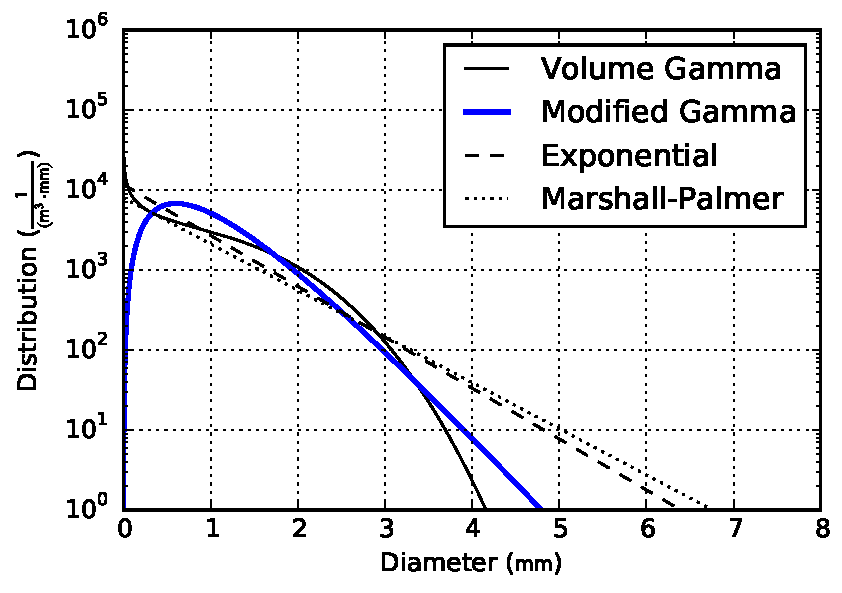
\includegraphics[scale=0.6]{figures/distribution-comparison.pdf}
	\end{center}
\end{frame}

\begin{frame}[<+->]
	\frametitle{Microphysics (cont.)}
	\begin{itemize}
		\item Much better to use modified gamma distribution (Ulbrich 1983)
		\item Three parameter distribution
		\begin{equation}
			N(D) = N_0 D^\mu e^{(-\Lambda D)}
		\end{equation}
		\item Only two moments $N_0 (<D^0>)$ and $q_r (<D^3>)$
	\end{itemize}
\end{frame}

\begin{frame}[<+->]
	\frametitle{Microphysics (cont.)}
	\begin{itemize}
		\item Attempted to use $\mu-\Lambda$ relation of Zhang et al. (2001)
		\begin{equation}
			\mu = \num{-0.016} \Lambda^2 + \num{1.213} \Lambda - \num{1.957}
		\end{equation}
		\item This yields a sixth order polynomial in $\Lambda$
		\item Though it generally has two real, positive roots
		\item Options for choosing root tested: min, max, closest to chosen $\Lambda$, closest to chosen $\mu$
	\end{itemize}
\end{frame}

\begin{frame}[<+->]
	\frametitle{Microphysics (cont.)}
	\begin{itemize}
		\item Instead, we add a constraint to conserve the (approximate) radar reflectivity factor of the model ($<D^6> = \frac{6}{\pi}^2<V^2>$)
		\item By combining the 0th, 3rd, and 6th moments of D we get:
		\begin{equation}
			\frac{\overline{D^3}^2}{\overline{D^0}\,\overline{D^6}} =  \frac{\nu + 1}{\nu + 2}
		\end{equation}
		\item This yields the following polynomial
		\begin{equation}
			\frac{\num{5}}{\num{6}} \mu^3 + \frac{\num{7}}{\num{2}} \mu^2 - \frac{\num{4}}{\num{3}} \mu - \num{14} = 0
		\end{equation}
		\item Which has a positive root of $\mu=\num{1.81}$
	\end{itemize}
\end{frame}

\begin{frame}
	\frametitle{Microphysics (cont.)}
	\begin{center}
		\includegraphics[scale=0.6]{figures/atten-distribution.pdf}
	\end{center}
\end{frame}

\section{Example Output}
\stepcounter{subsection}
\begin{frame}
	\frametitle{Model Field}
	\begin{center}
		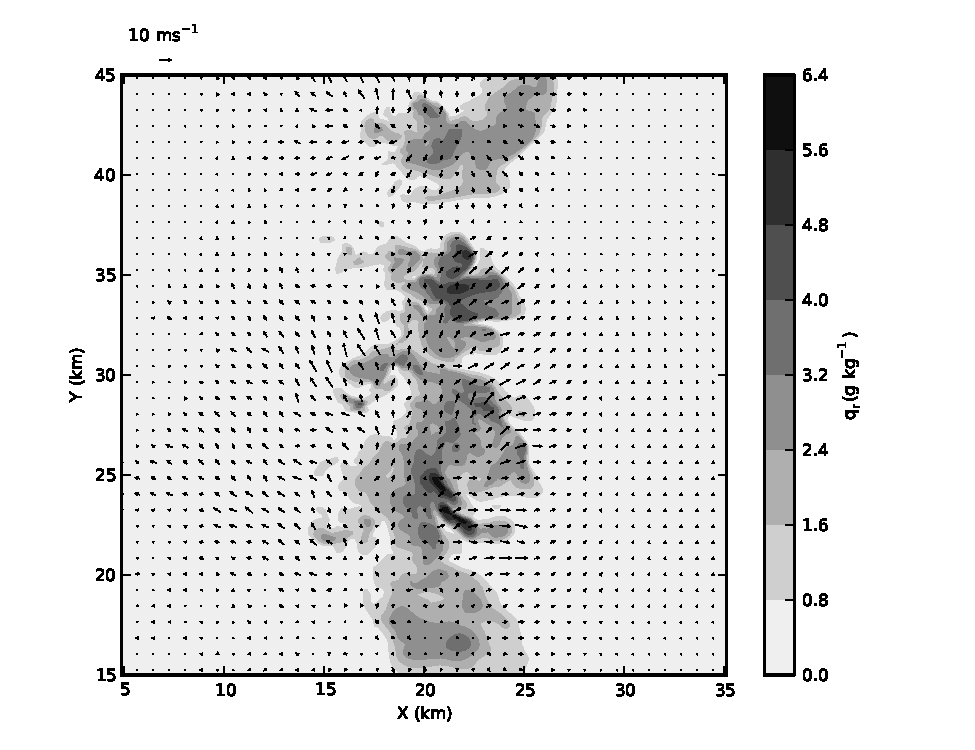
\includegraphics[scale=0.5]{figures/commas_wz_3600_qr_wind_vectors.pdf}	
	\end{center}
\end{frame}

\begin{frame}
	\frametitle{Example Configuration}
	\begin{center}
	    \begin{tabular}{ | l | l | }
	        \hline
	        Antenna gain & \SI{45.5}{dB} \\
	        Peak power & \SI{250}{\kilo\watt} \\
	        First range gate & \SI{500}{\meter} \\
	        Noise power & \SI{-113}{dBm} \\
	        Elevation & \SI{0.5}{\degree} \\
	        PRT & \SI{0.667}{\milli\second} \\
	        Rotation Rate & \SI{20}{\degree\per\second} \\
	        Pulses per radial & \num{75} \\
	        Gate length & \SI{125}{\meter} \\
	        Antenna Limits & Main-lobe only \\
			Wavelength &  \SI{5.5}{\centi\meter} \\
			Beamwidth & \SI{1.0}{\degree} \\
			Radial Spacing & \SI{1.0}{\degree} \\
			\hline
	    \end{tabular}
	\end{center}
\end{frame}

\begin{frame}
	\frametitle{Example Images}
	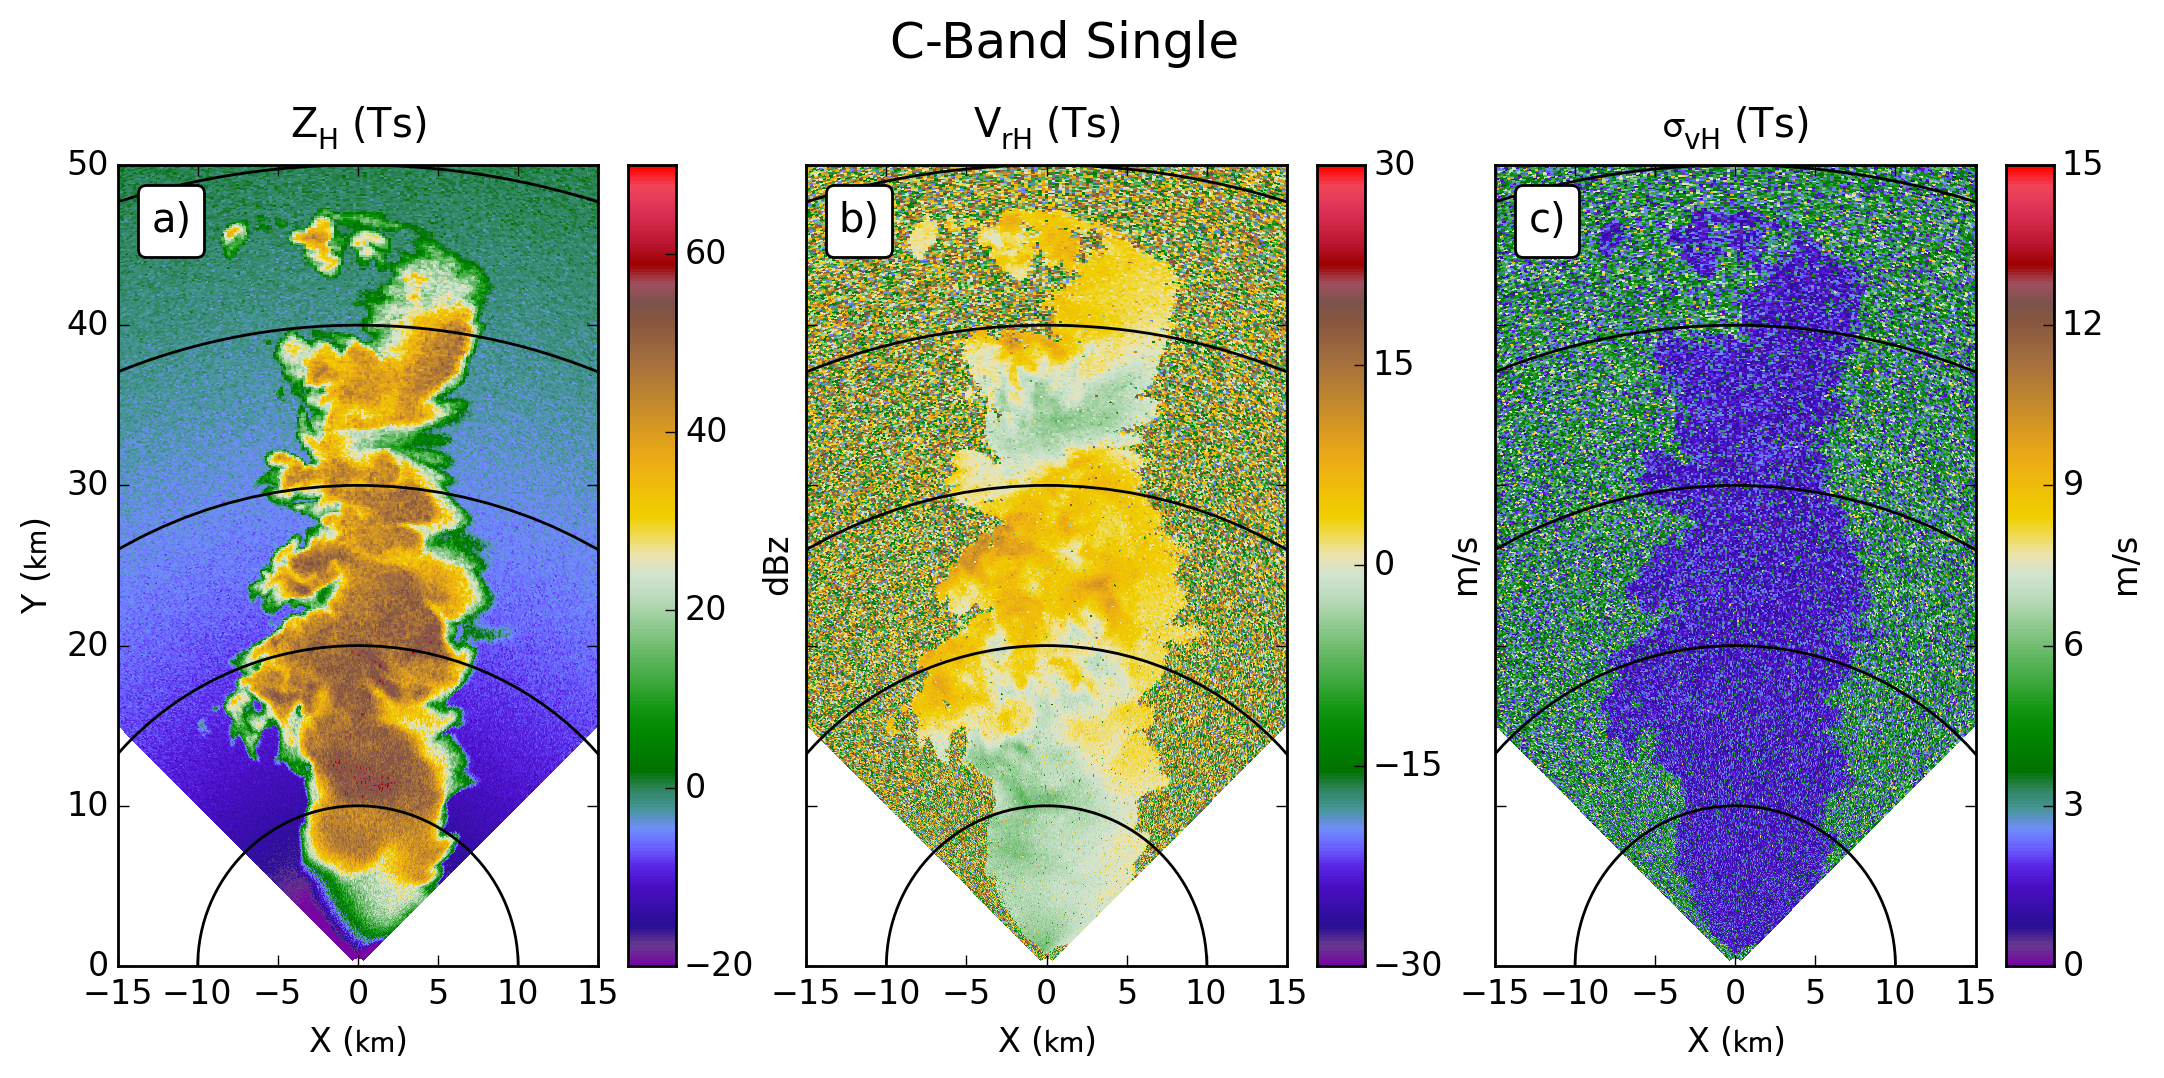
\includegraphics[scale=0.4]{figures/C_Single.png}
\end{frame}

\begin{frame}
	\frametitle{Example Images (cont.)}
	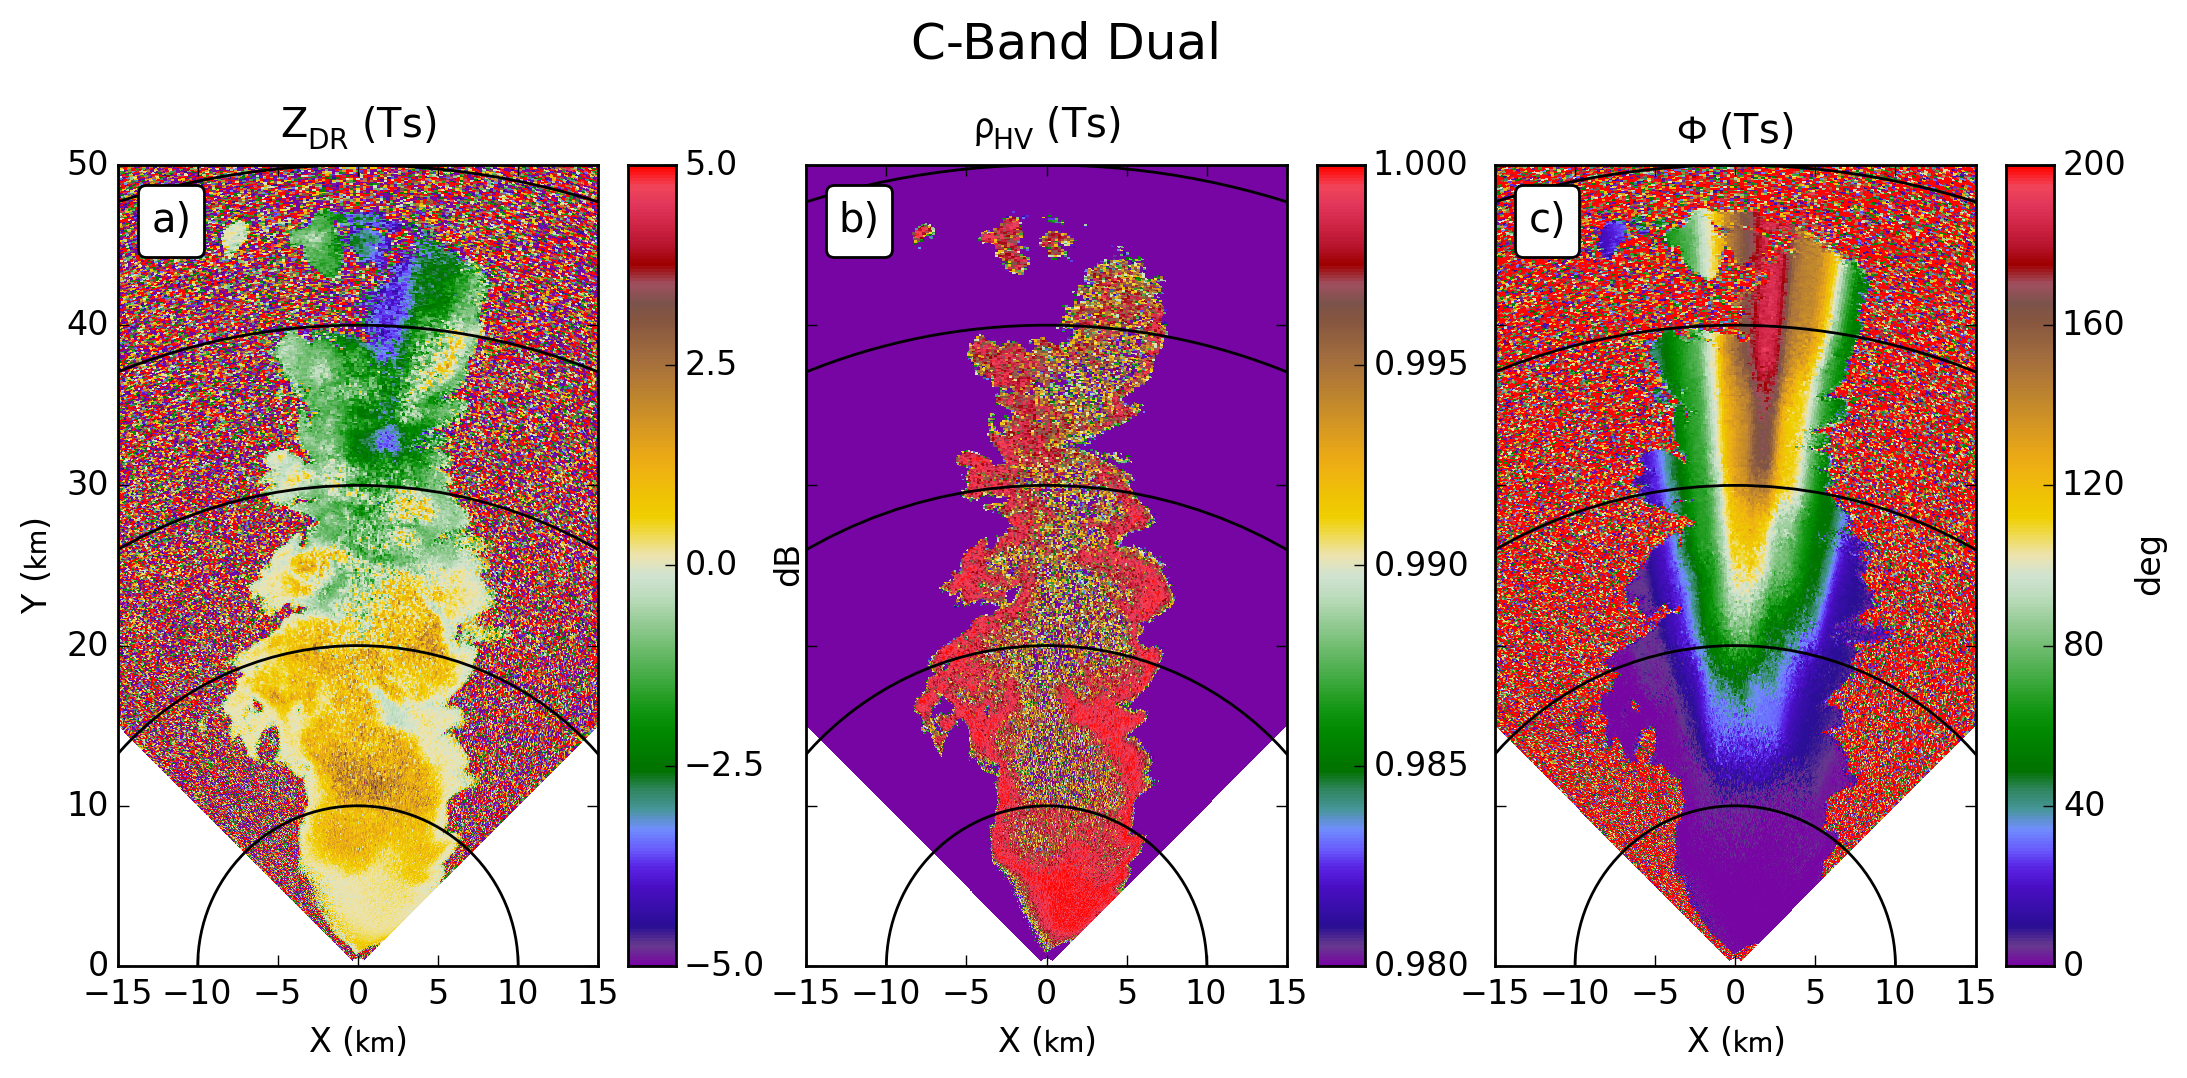
\includegraphics[scale=0.4]{figures/C_Dual.png}
\end{frame}

\begin{frame}
	\frametitle{Example Images (cont.)}
	\begin{center}
		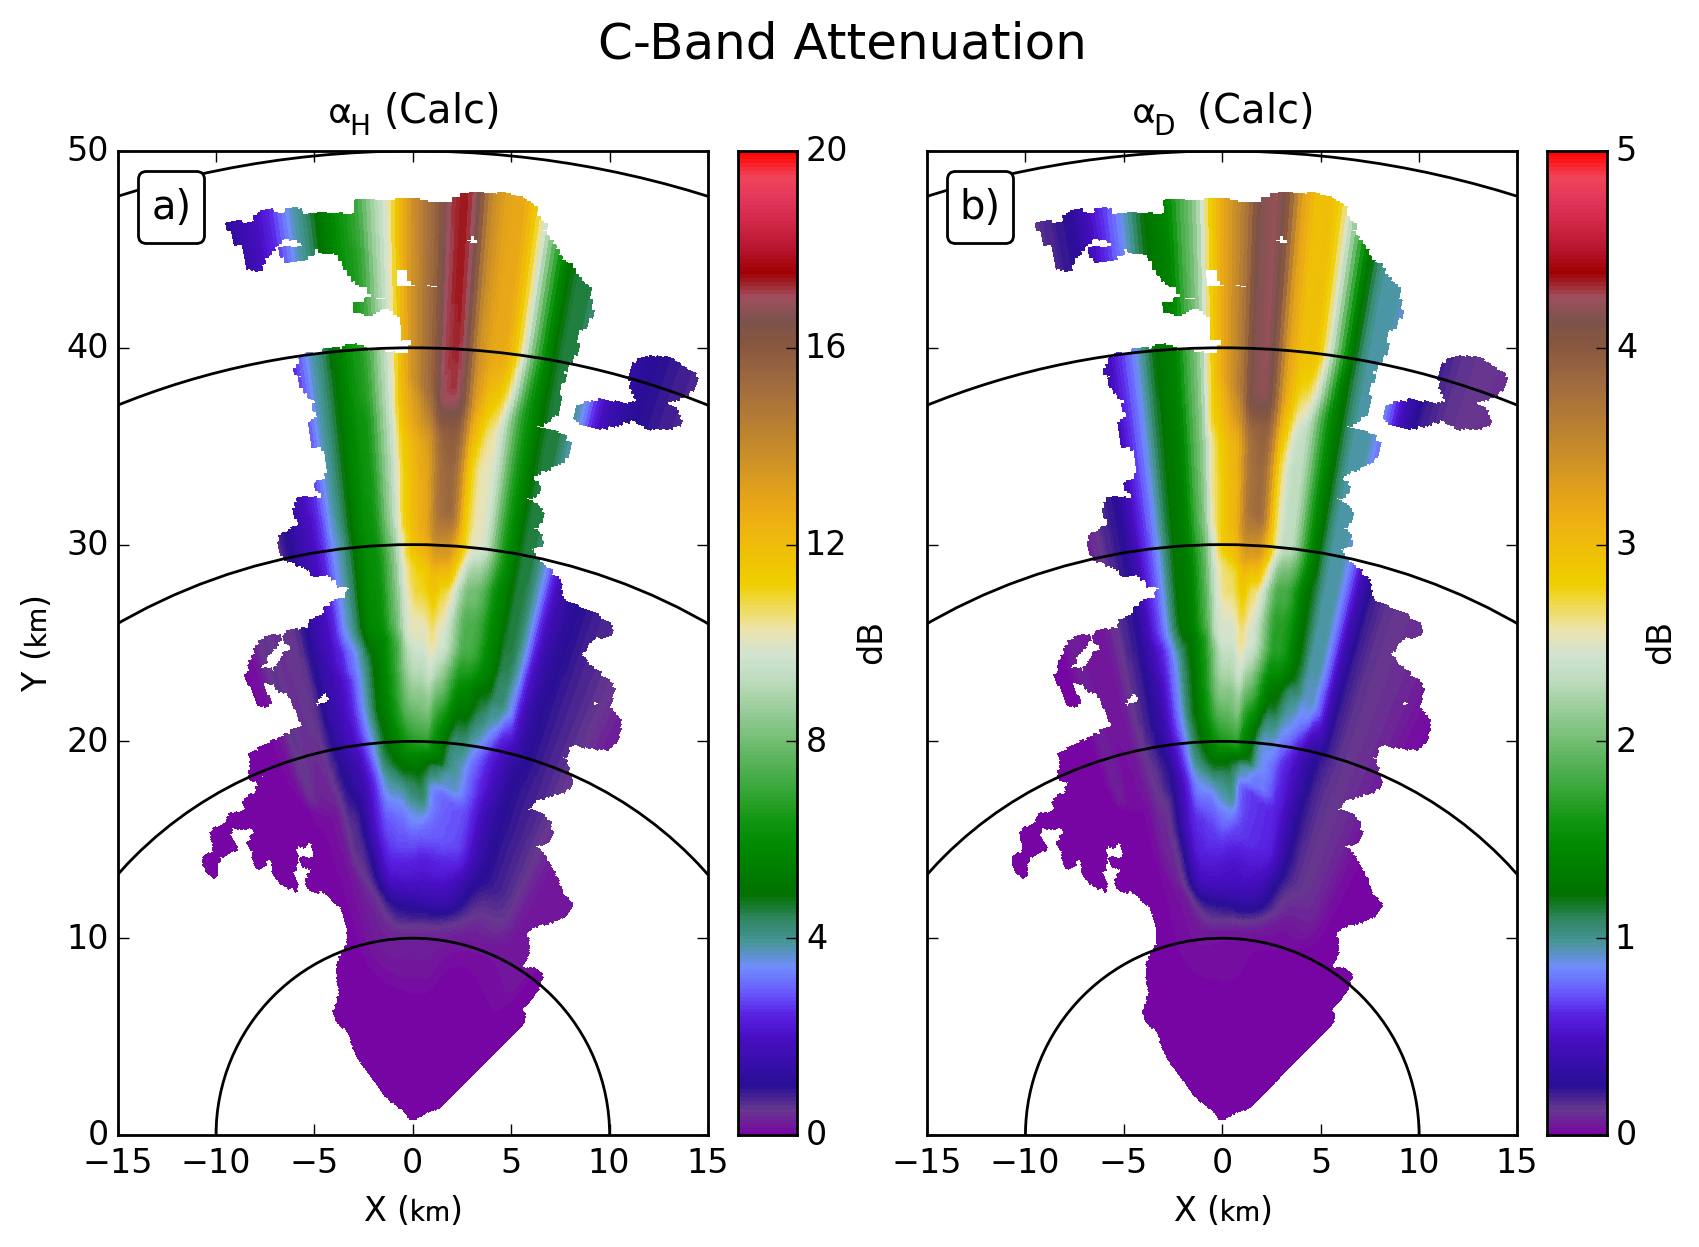
\includegraphics[scale=0.4]{figures/C_Attenuation.png}
	\end{center}
\end{frame}

\begin{frame}
	\frametitle{Example Images (cont.)}
	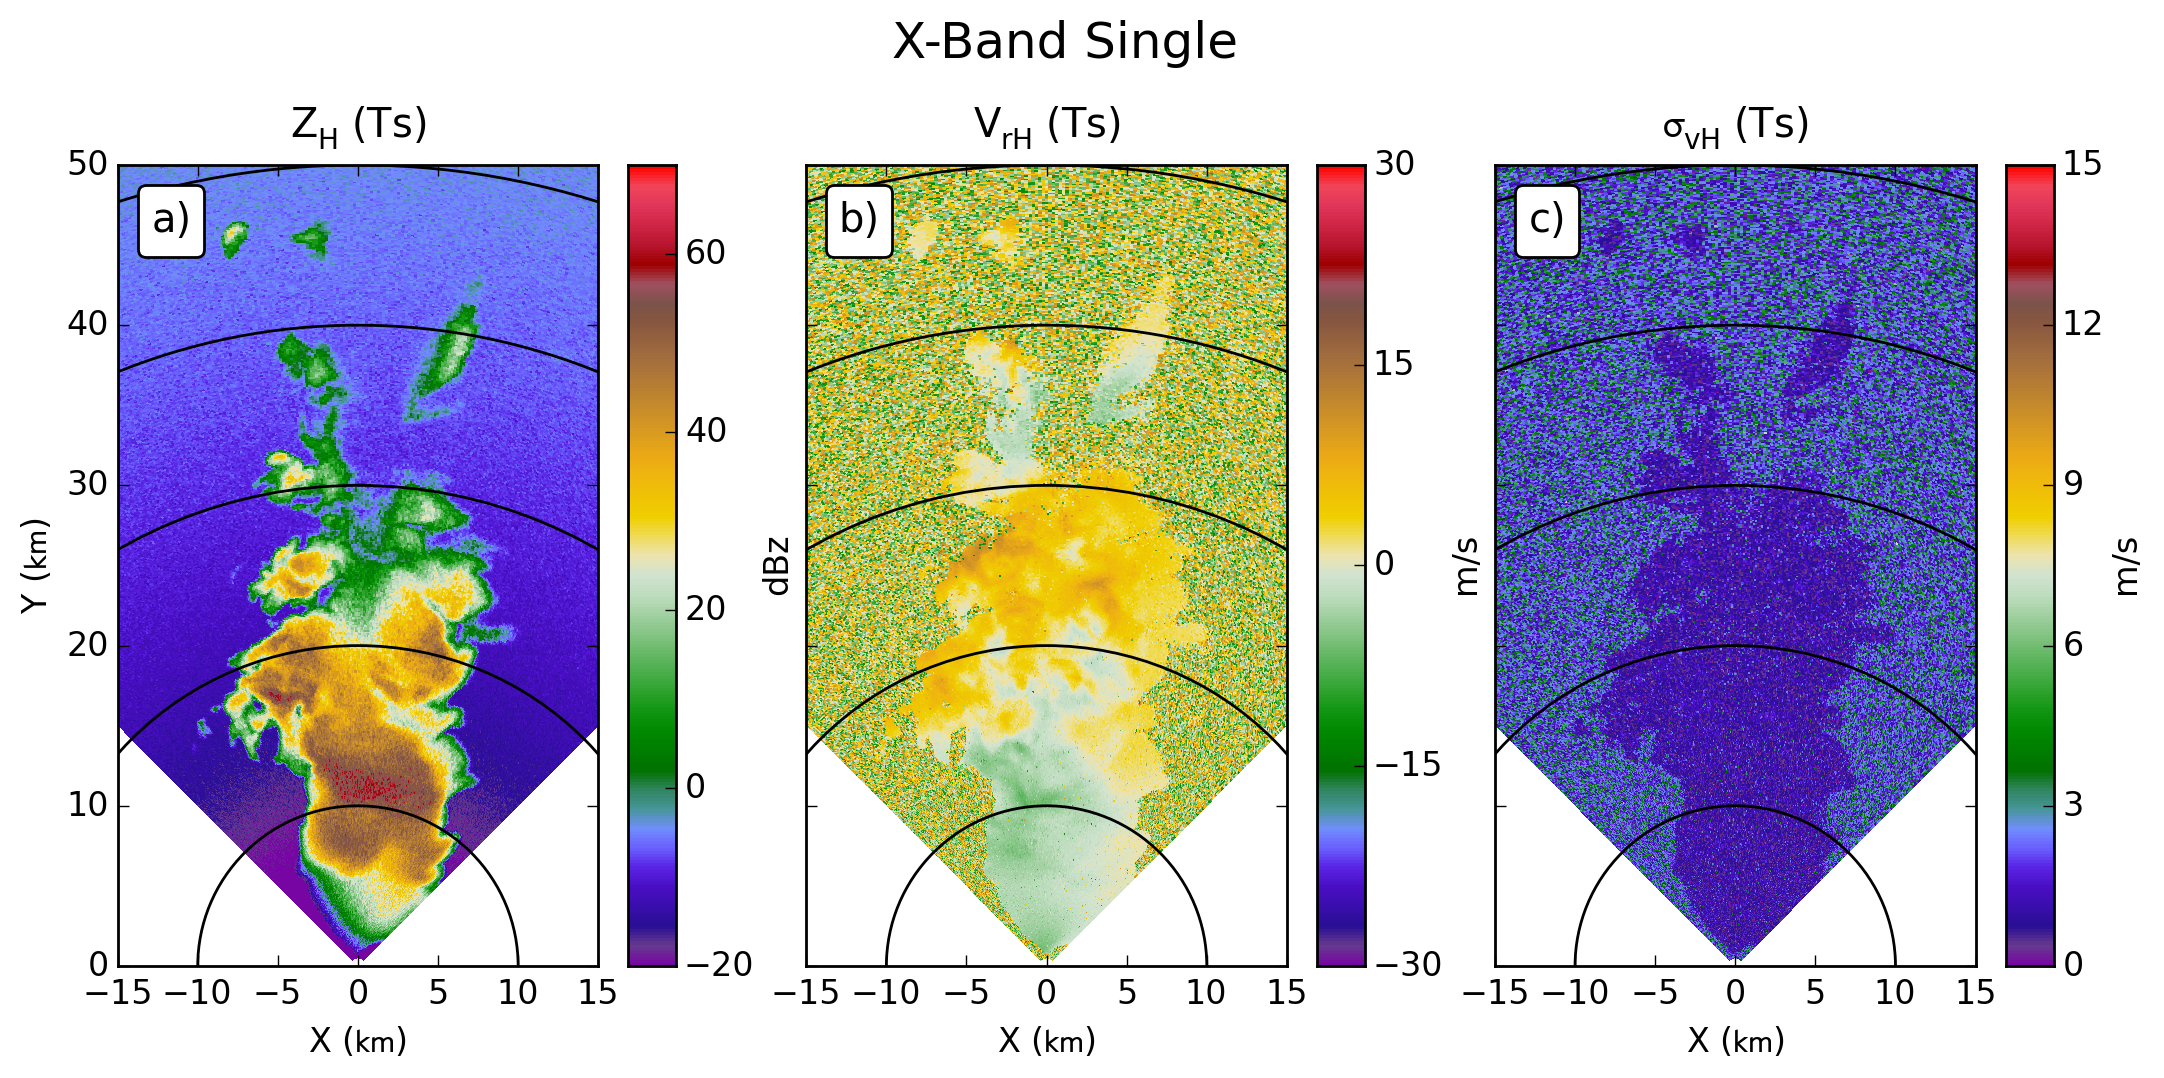
\includegraphics[scale=0.4]{figures/X_Single.png}
\end{frame}

\begin{frame}
	\frametitle{Example Images (cont.)}
	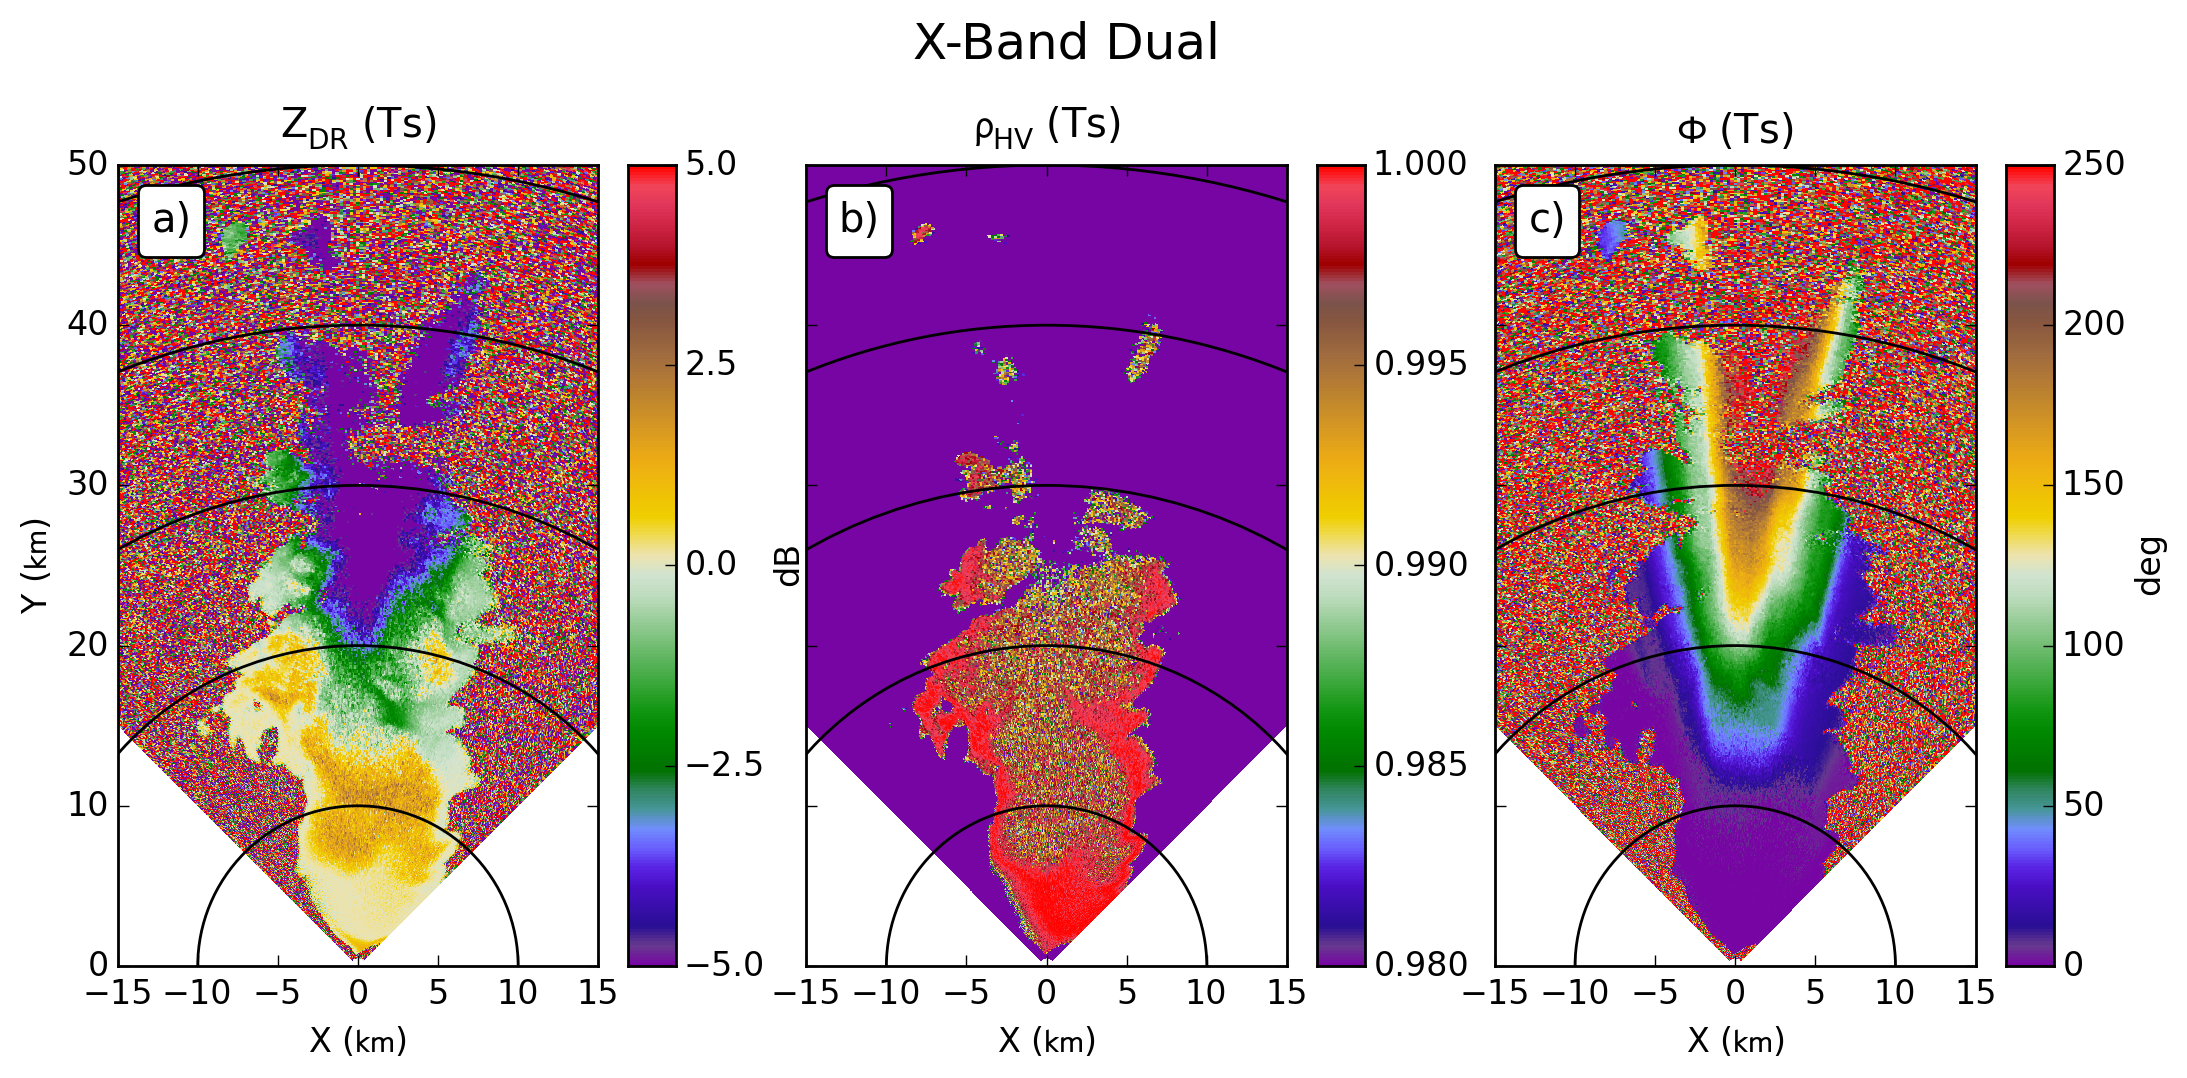
\includegraphics[scale=0.4]{figures/X_Dual.png}
\end{frame}

\begin{frame}
	\frametitle{Example Images (cont.)}
	\begin{center}
		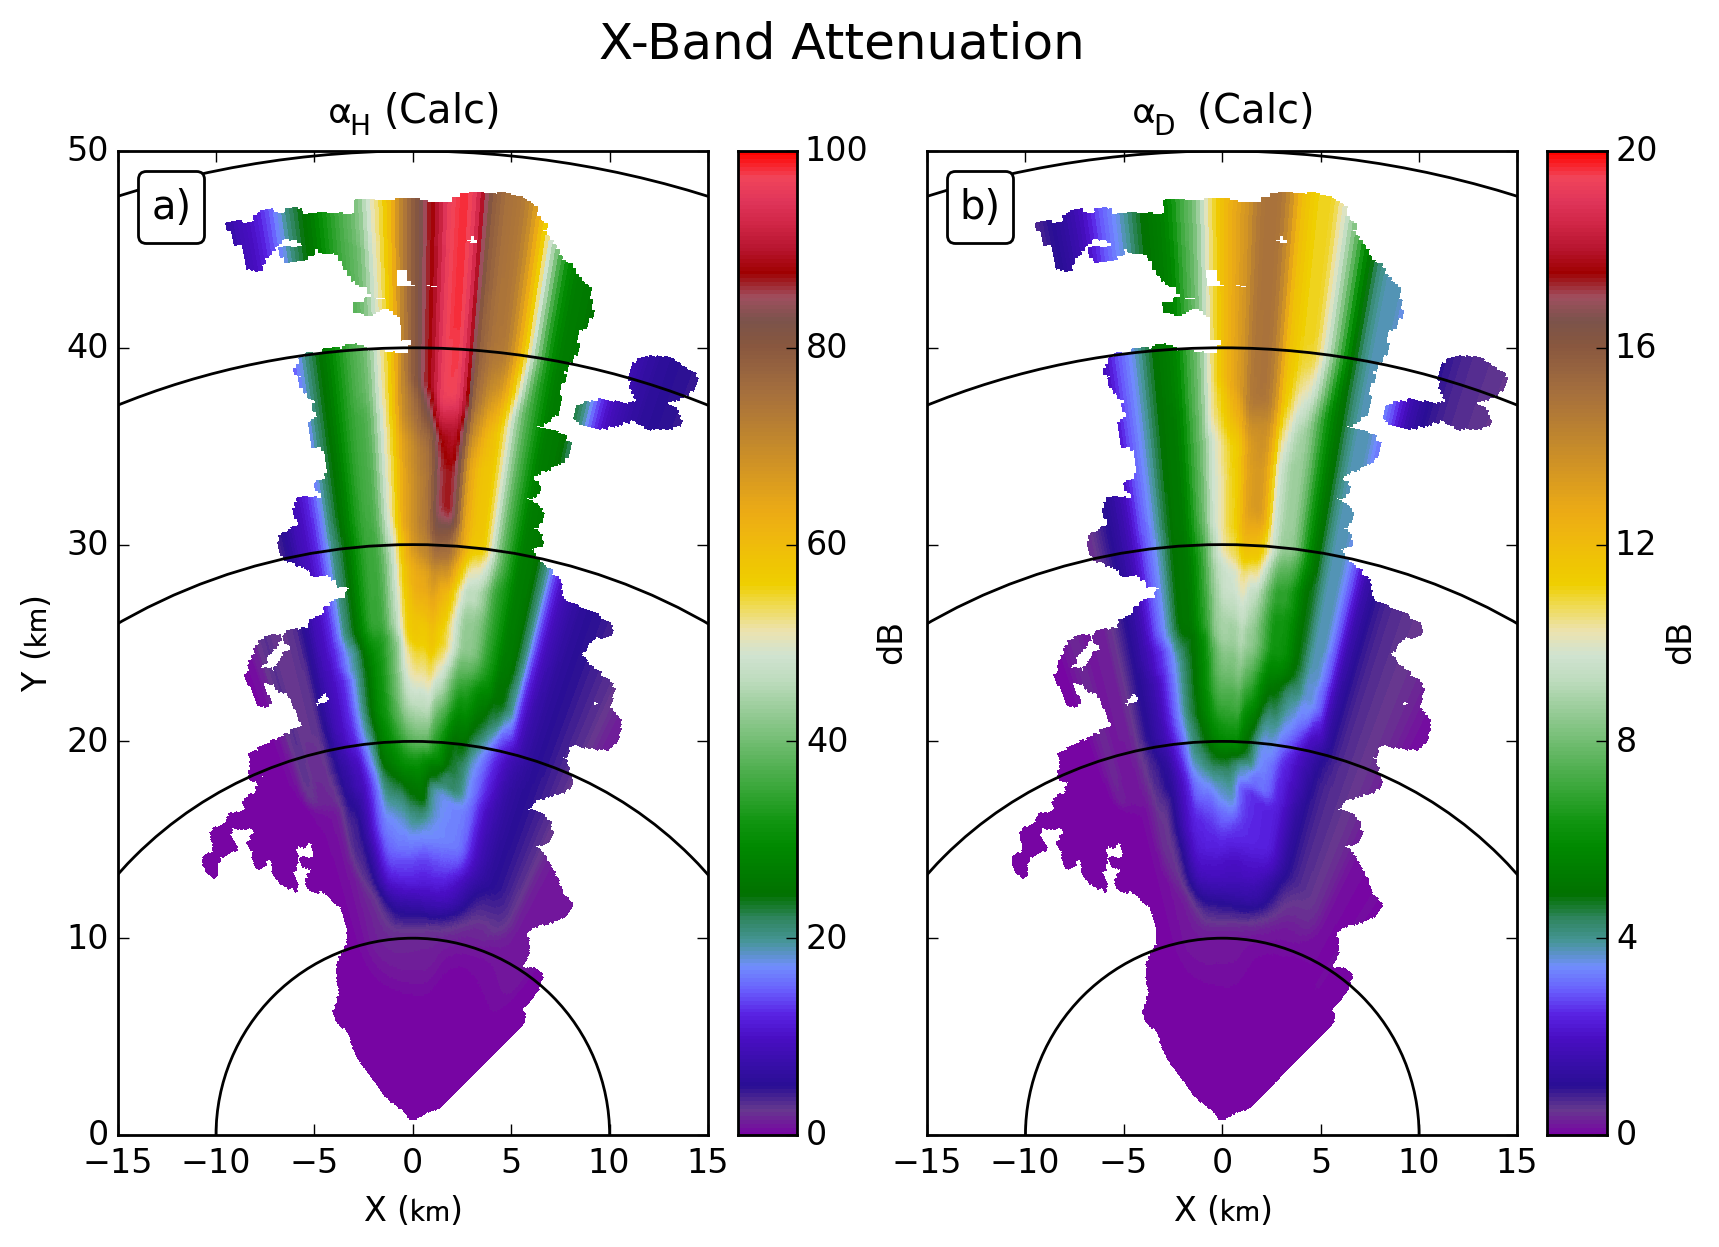
\includegraphics[scale=0.4]{figures/X_Attenuation.png}
	\end{center}
\end{frame}

\section{Algorithms}
\stepcounter{subsection}
\begin{frame}
	\frametitle{Linear $\Phi_{DP}$}
	\begin{itemize}
		\item Described by Bringi et al. (1990)
		\item Formulate linear relationship between $K_{DP}$ and $A_H$
		\begin{align*}
			A_H &= \beta_H K_{DP} \\
			A_D &= \beta_D K_{DP}
		\end{align*}
		\item Leads to direct conversion between $\Phi_{DP}$  and  both
				$\alpha_H$ and $\alpha_D$
	\end{itemize}
\end{frame}

\begin{frame}
	\frametitle{ZPHI}
	\begin{itemize}
		\item Described by Testud et al. (2000)
		\item Based around Hitschfeld (1954) reflectivity-based method
		\item Uses linear $\Phi_{DP}$ to provide constraint
			\begin{align*}
			I(r, r_0) &= \num{0.46}b\int_r^{r_0}Z_a^b(s)\,ds \\
			\alpha(r_0) &= \frac{Z_a^b(r_0)}{I(r_1,r_0)} \lbrace 10^{\num{0.1}b\gamma\Delta\Phi} - 1\rbrace \\
			\alpha(r) &= \frac{Z_a^b(r)}{I(r_1,r_0) + \lbrace 10^{\num{0.1}b\gamma\Delta\Phi} - 1\rbrace I(r, r_0)}
			  \times \lbrace 10^{\num{0.1}b\gamma\Delta\Phi} - 1\rbrace
			\end{align*}
	\end{itemize}
\end{frame}

\begin{frame}
	\frametitle{Self-Consistent}
	\begin{itemize}
		\item Described by Bringi et al. (2001)
		\item Adds a "self-consistent" restriction to ZPHI
		\item Attempts to automatically find the optimal value of $\gamma$
			 \begin{align*}
			\phi_{DP}^c(r;\gamma) &= 2 \int_{r_0}^r \frac{A_h(s;\gamma)}{\gamma}\,ds \\
			\gamma_{min} &\leq \gamma \leq \gamma_{max} \\
			Error &= \sum_{j=1}^N \left| \Phi_{DP}^{filt}(r_j) - \Phi_{DP}^c(r_j;\gamma) \right|
			\end{align*}
	\end{itemize}
\end{frame}

\begin{frame}[<+->]
	\frametitle{Coefficient Regression}
	\begin{itemize}
		\item Need to determine own set of coefficients for algorithms
		\item Original algorithms all use different assumptions
		\item All relations some kind of power law
		\item Make best-case coefficients using actual data from model and
		the assumptions used in simulation
	\end{itemize}
\end{frame}

\begin{frame}
	\frametitle{Coefficient Regression (cont.)}
	\begin{center}
		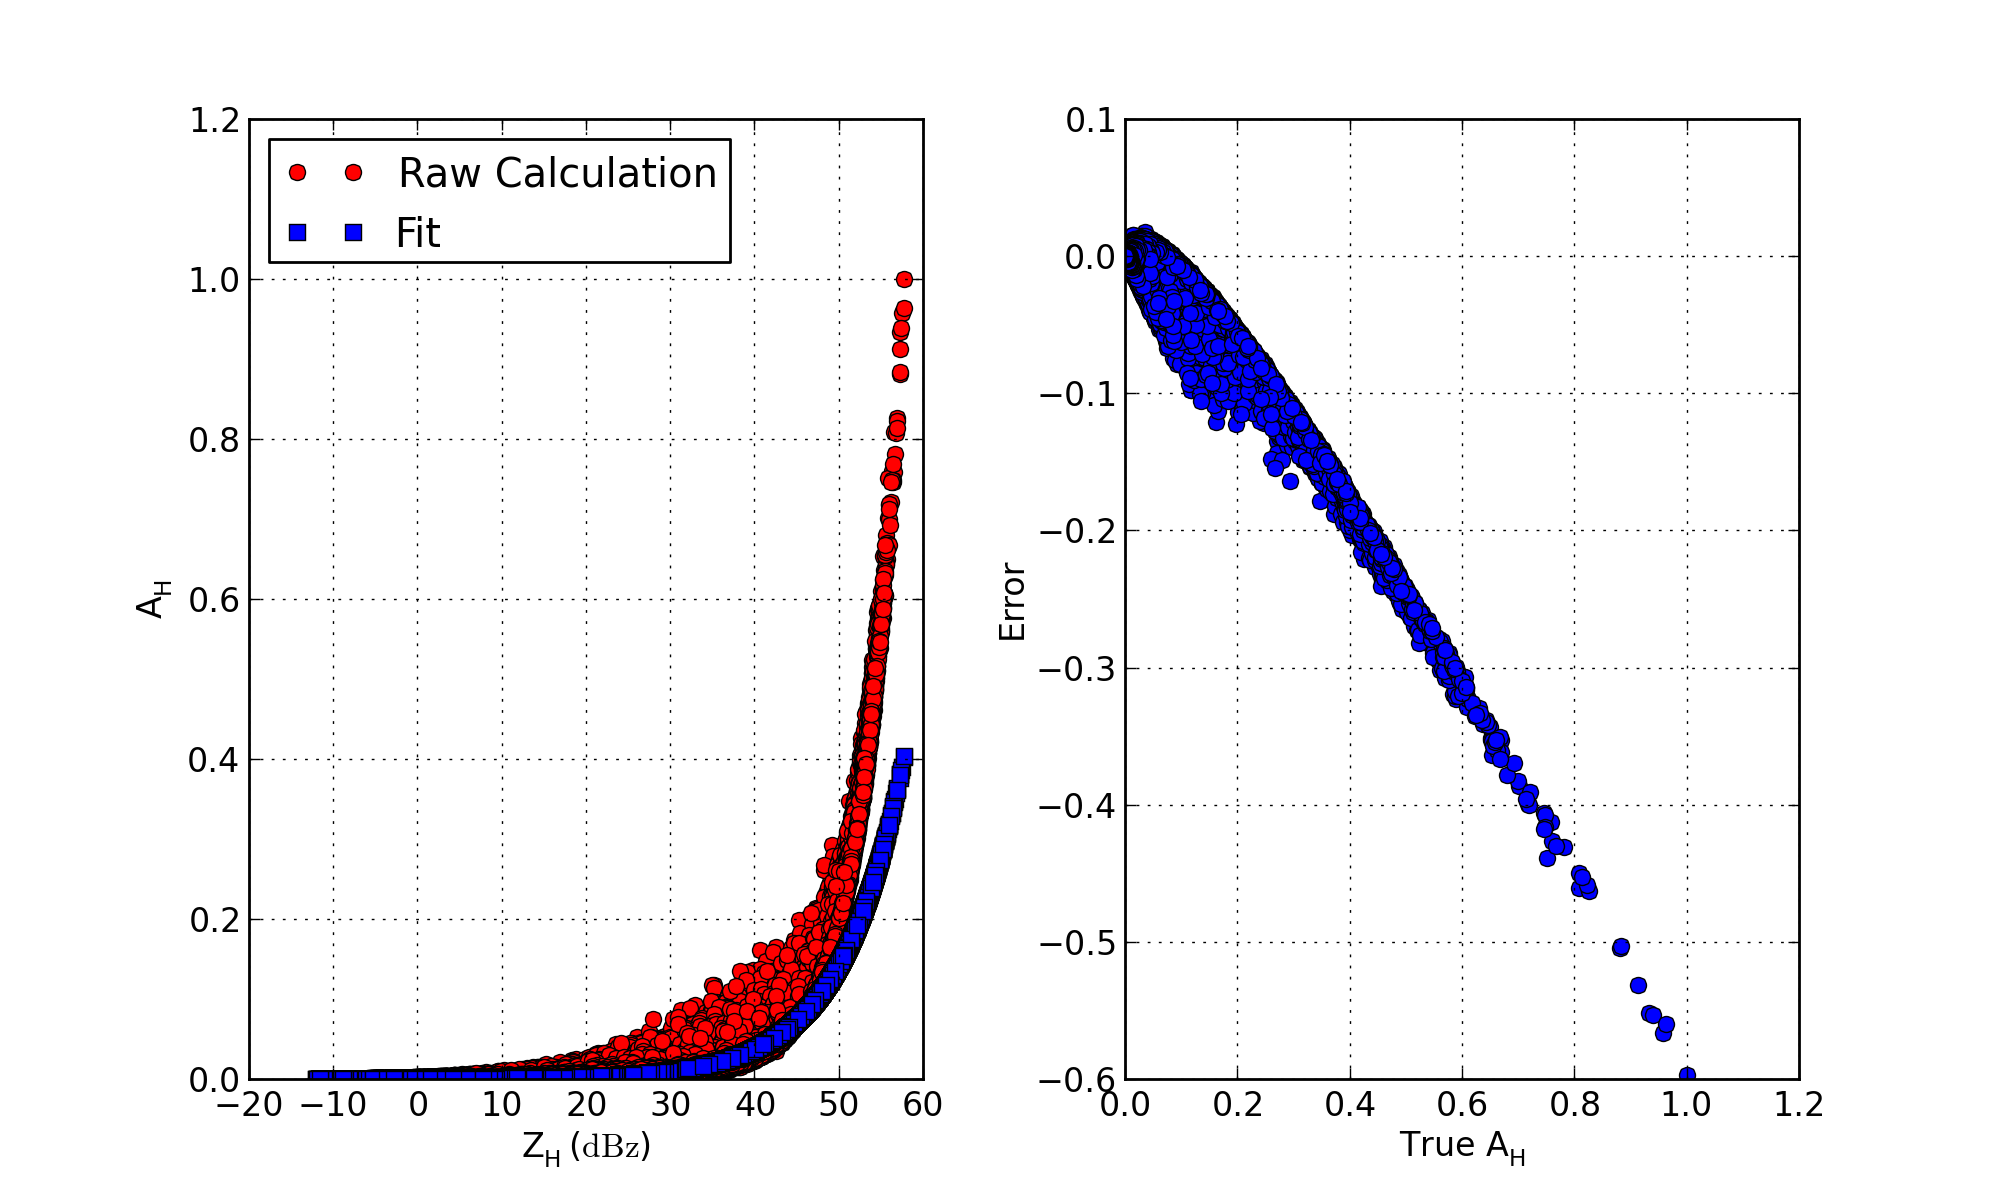
\includegraphics[scale=0.35]{figures/basic_power_law.png}
	\end{center}
	\begin{itemize}
		\item Clearly bias in the fit curve
	\end{itemize}
\end{frame}

\begin{frame}
	\frametitle{Coefficient Regression (cont.)}
	\begin{center}
		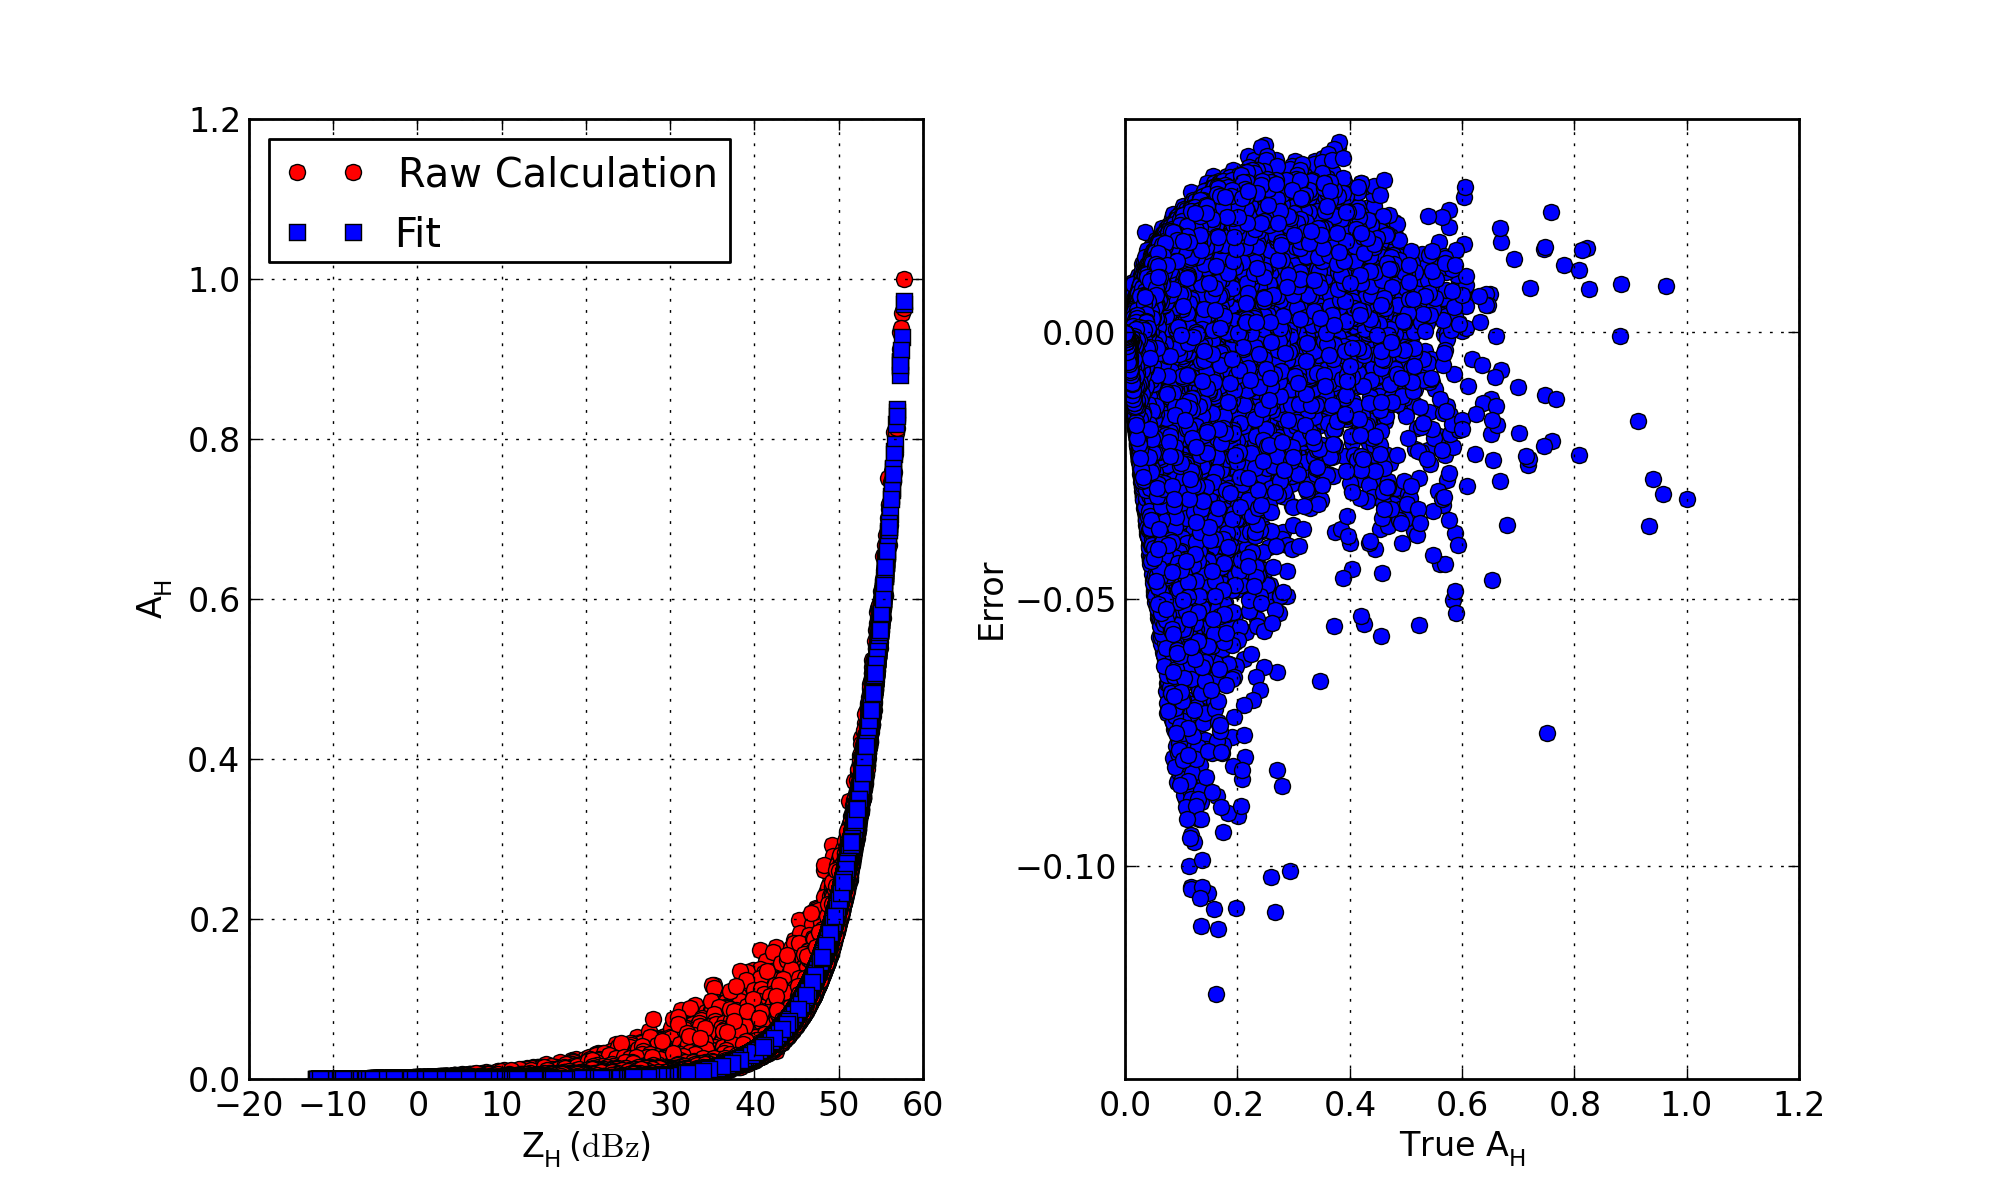
\includegraphics[scale=0.35]{figures/weighted_power_law.png}
	\end{center}
	\begin{itemize}
		\item Much better when using $A_H^2$ as the weights in regression
	\end{itemize}
\end{frame}

\section{Errors}
\stepcounter{subsection}
\subsection{Model Errors}
\begin{frame}
	\frametitle{Experimental Configuration}
	\begin{center}
	    \begin{tabular}{ | l | l | }
	        \hline
	        Antenna gain & \SI{45.5}{dB} \\
	        Peak power & \SI{250}{\kilo\watt} \\
	        First range gate & \SI{500}{\meter} \\
	        Noise power & \SI{-113}{dBm} \\
	        Elevation & \SI{0.5}{\degree} \\
	        PRT & \SI{0.667}{\milli\second} \\
	        Rotation Rate & \SI{20}{\degree\per\second} \\
	        Pulses per radial & \num{75} \\
	        Gate length & \SI{100}{\meter} \\
	        Antenna Limits & Main-lobe only \\
			Beamwidth & \SI{0.25}{\degree} \\
			Radial Spacing & \SI{0.25}{\degree} \\
			Scattering Model & T-Matrix \\
			\hline
	    \end{tabular}
	\end{center}
\end{frame}

\subsubsection{Control}
\begin{frame}
	\frametitle{Control: Matched Assumptions}
	\begin{center}
	    \begin{tabular}{ | l | l | }
	        \hline
	        Temperature & \SI{283}{\kelvin} \\
	        Drop Shape Model & Brandes \\
	        Wavelength & \SI{5.5}{\centi\meter}, \SI{3.21}{\centi\meter} \\
			\hline
	    \end{tabular}
	\end{center}	
\end{frame}

\begin{frame}
    \begin{center}
        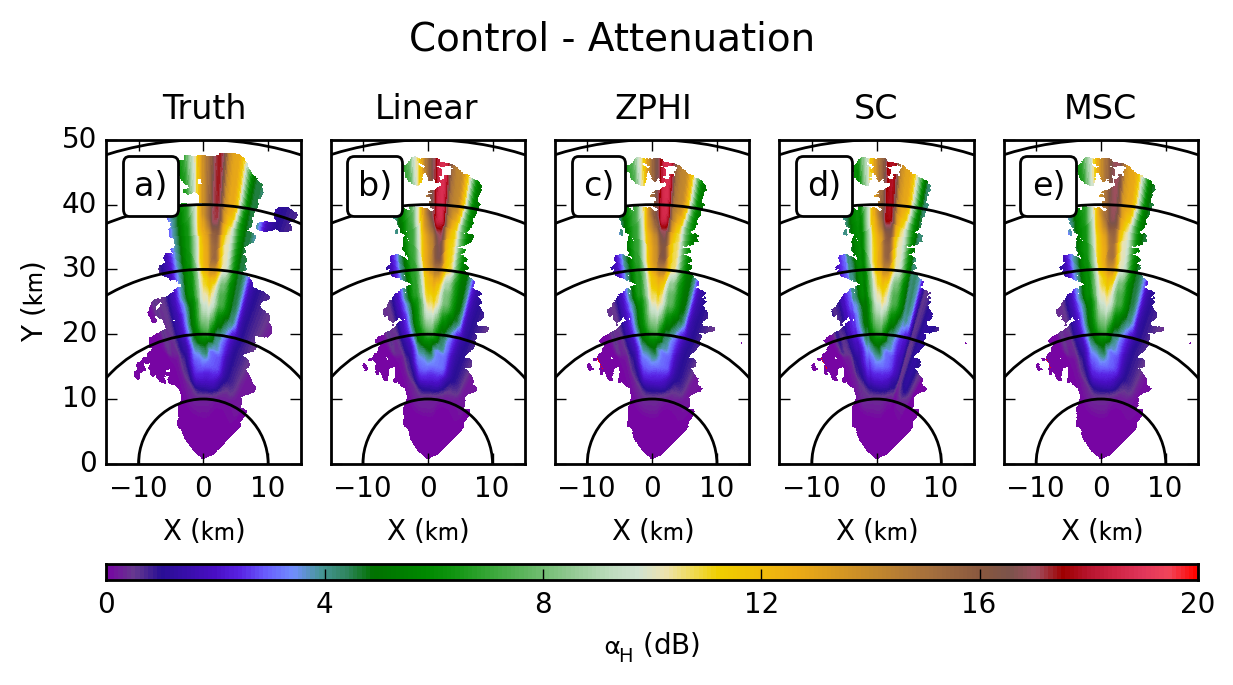
\includegraphics[scale=0.7]{figures/C_Control_Attenuation_H}
    \end{center}
\end{frame}

\begin{frame}
    \begin{center}
        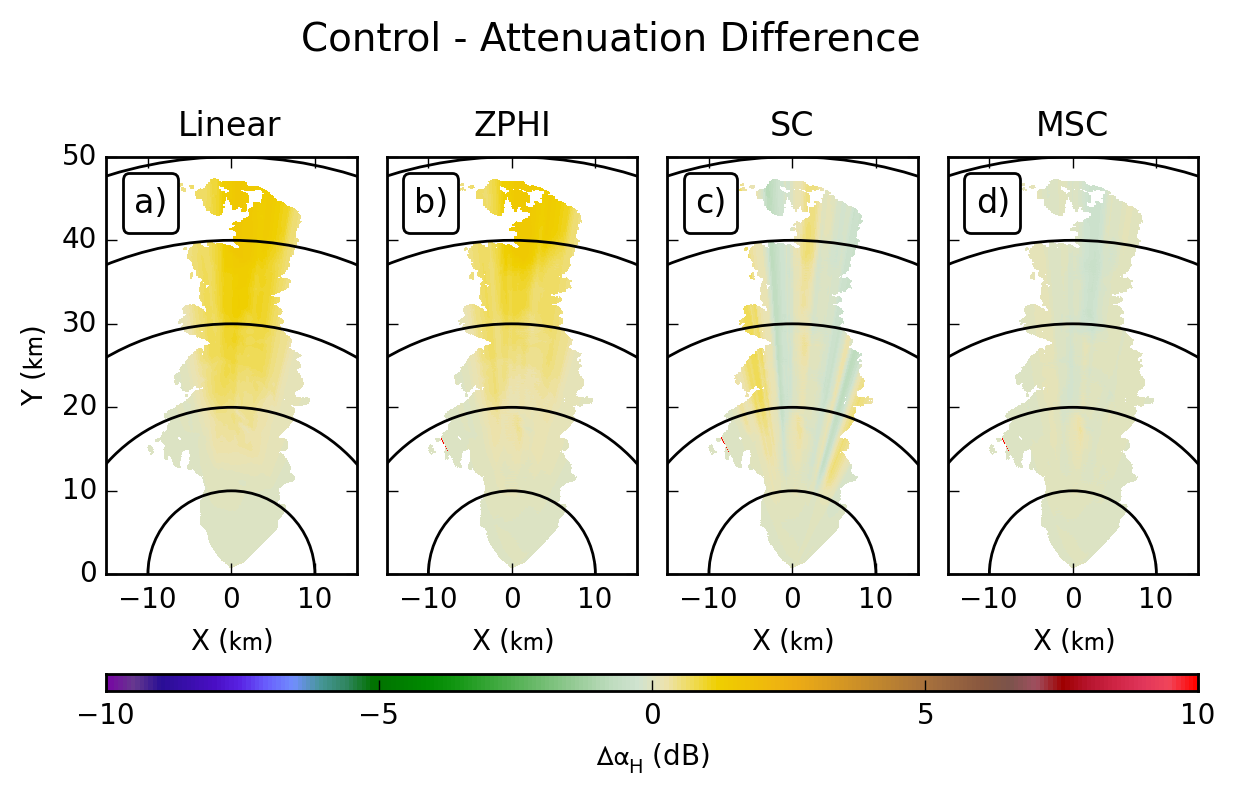
\includegraphics[scale=0.7]{figures/C_Control_Attenuation_Difference_H}
    \end{center}
\end{frame}

\begin{frame}
    \begin{center}
        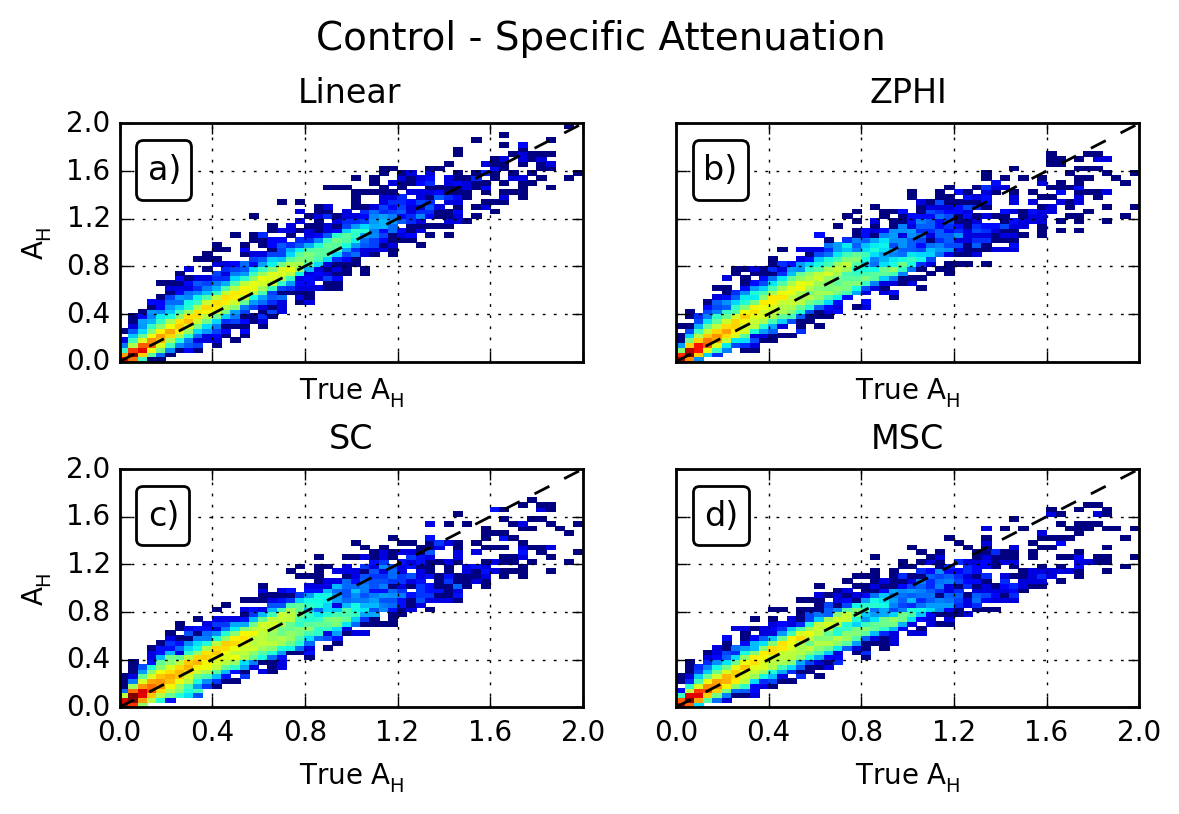
\includegraphics[scale=0.7]{figures/C_Control_Specific_Attenuation_H_scatter}
    \end{center}
\end{frame}

\begin{frame}
    \begin{center}
        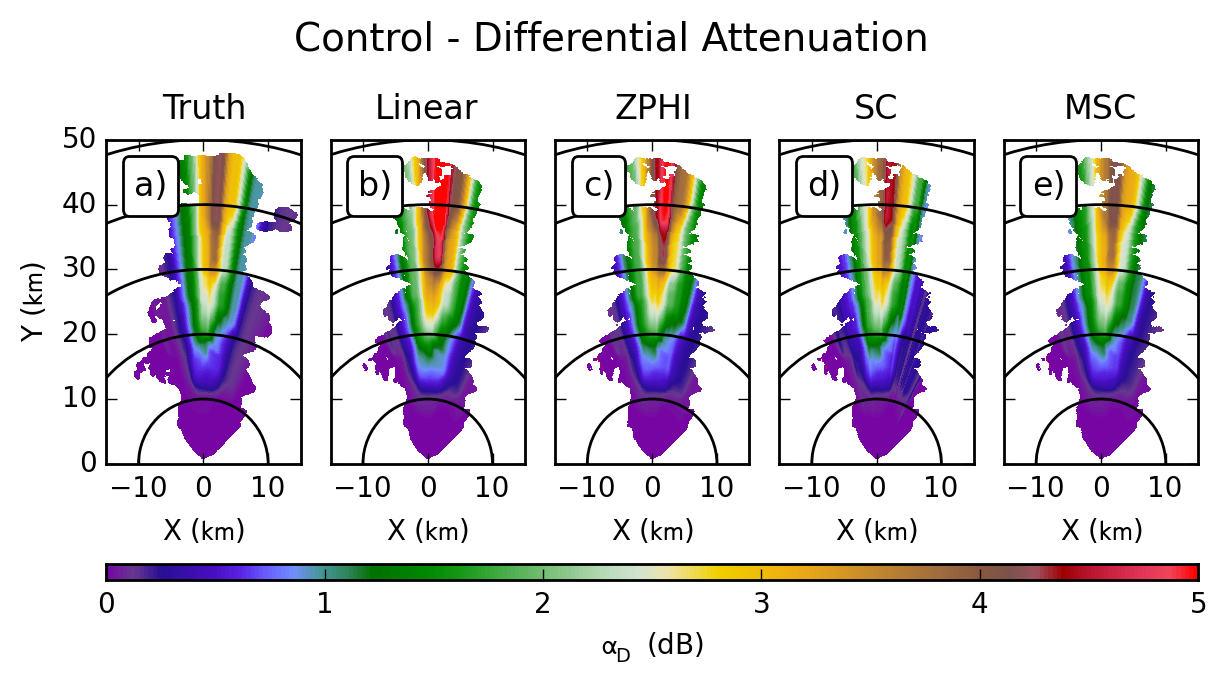
\includegraphics[scale=0.7]{figures/C_Control_Differential_Attenuation}
    \end{center}
\end{frame}

\begin{frame}
    \begin{center}
        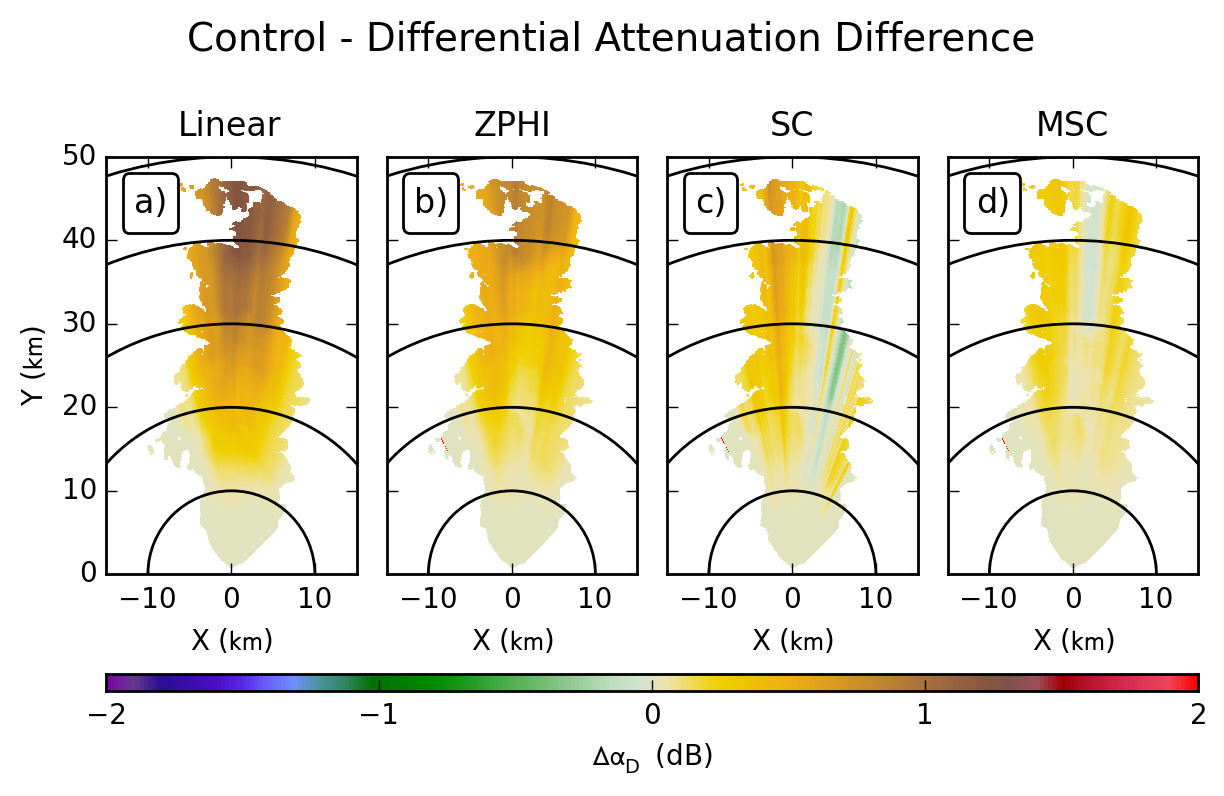
\includegraphics[scale=0.7]{figures/C_Control_Differential_Attenuation_Difference}
    \end{center}
\end{frame}

\begin{frame}
    \begin{center}
        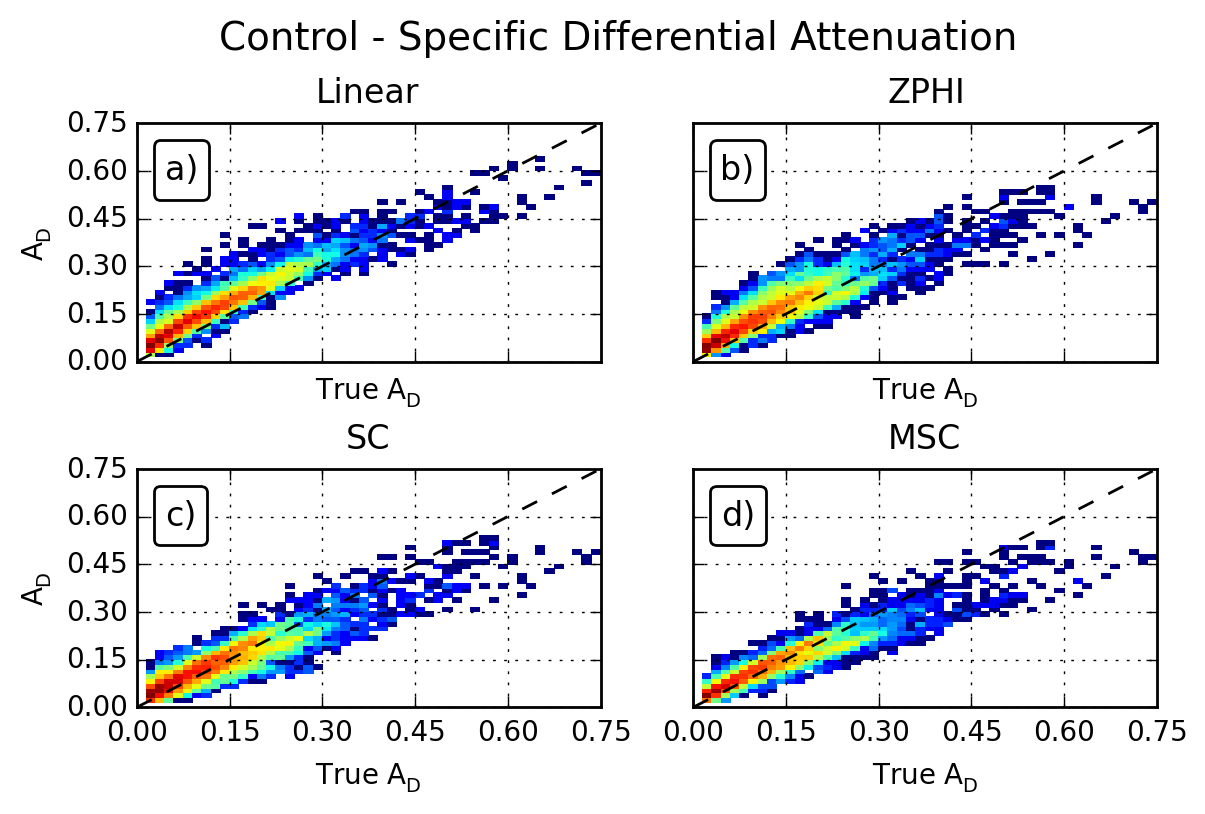
\includegraphics[scale=0.7]{figures/C_Control_Specific_Differential_Attenuation_scatter}
    \end{center}
\end{frame}

\begin{frame}
    \begin{center}
        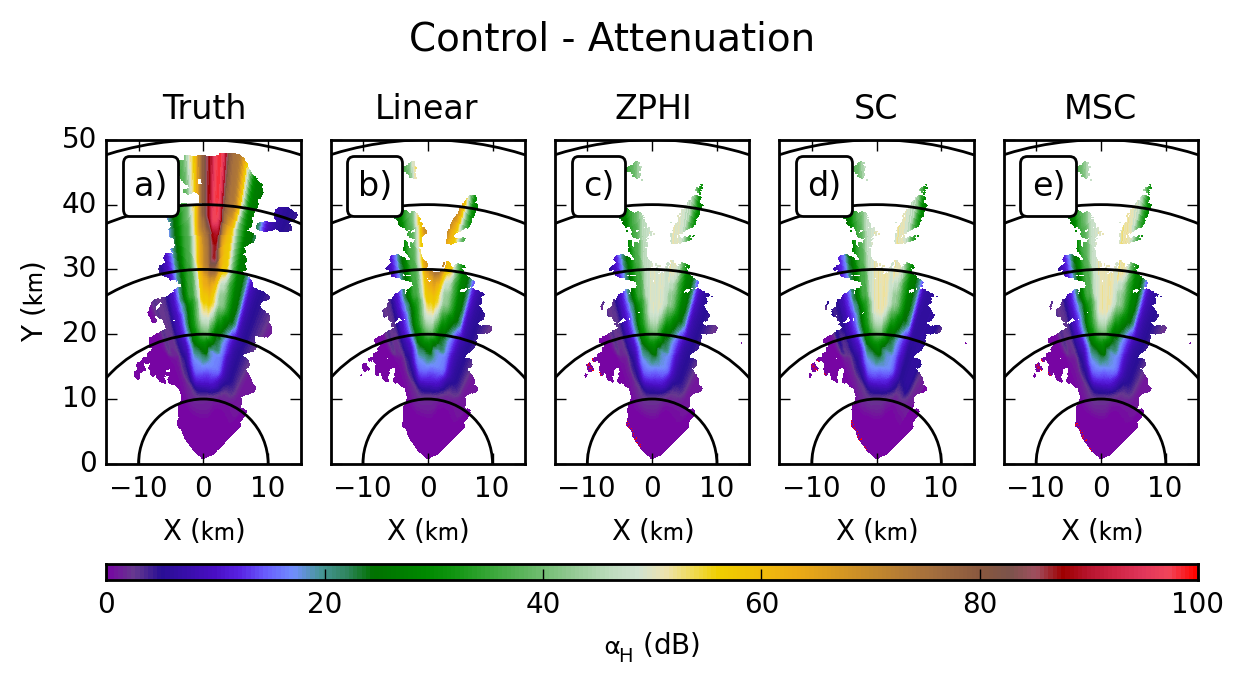
\includegraphics[scale=0.7]{figures/X_Control_Attenuation_H}
    \end{center}
\end{frame}

\begin{frame}
    \begin{center}
        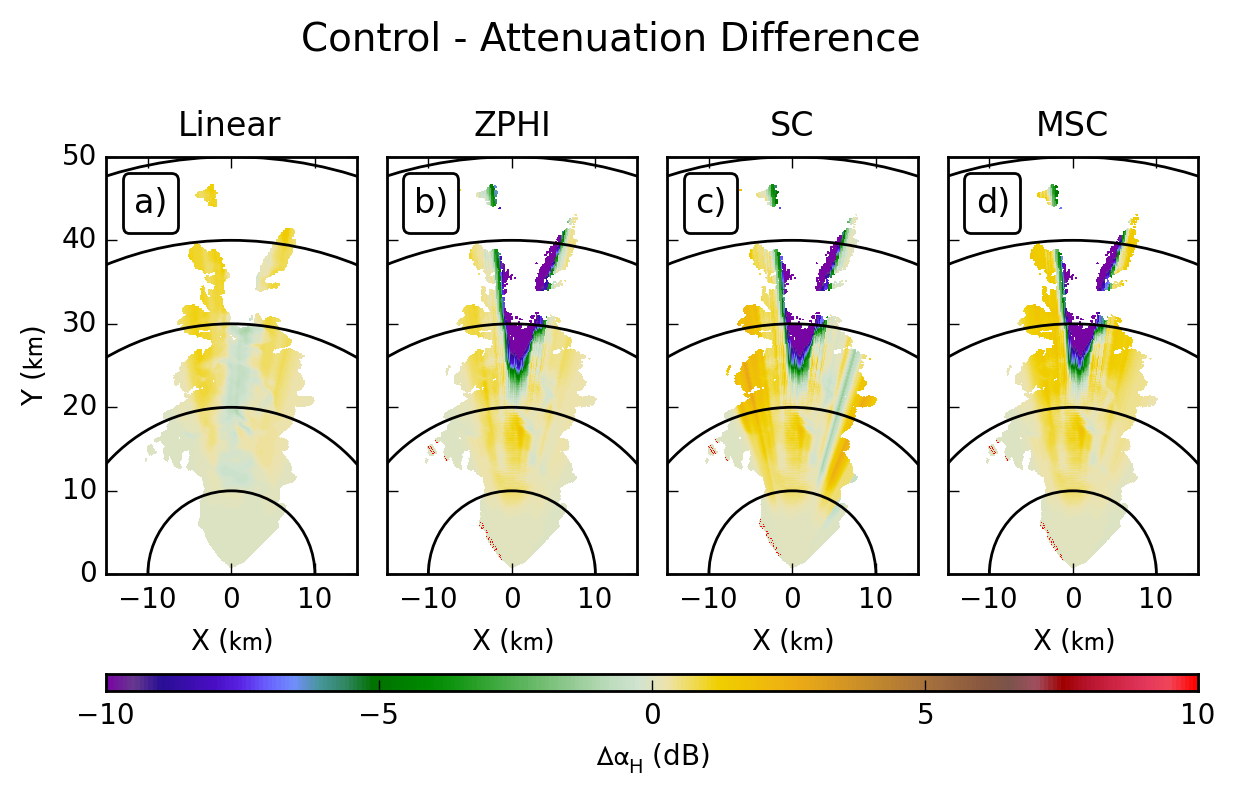
\includegraphics[scale=0.7]{figures/X_Control_Attenuation_Difference_H}
    \end{center}
\end{frame}

\begin{frame}
    \begin{center}
        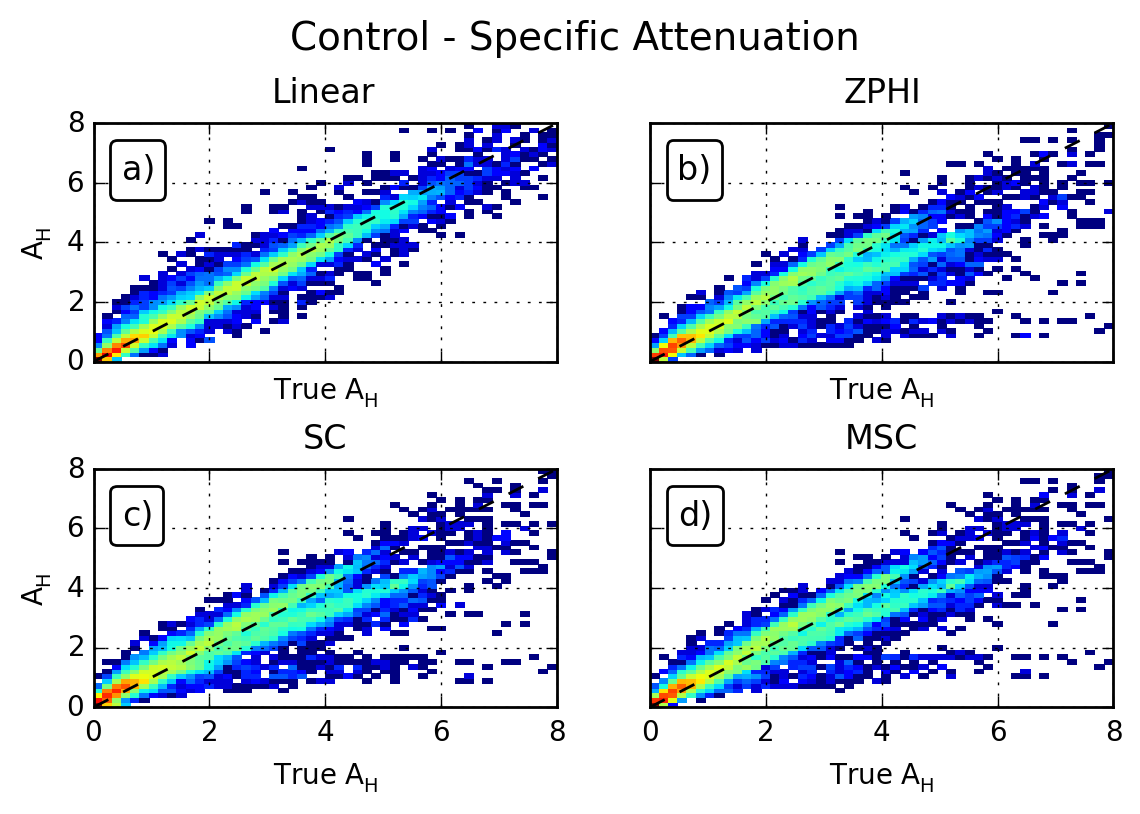
\includegraphics[scale=0.7]{figures/X_Control_Specific_Attenuation_H_scatter}
    \end{center}
\end{frame}

\begin{frame}
    \begin{center}
        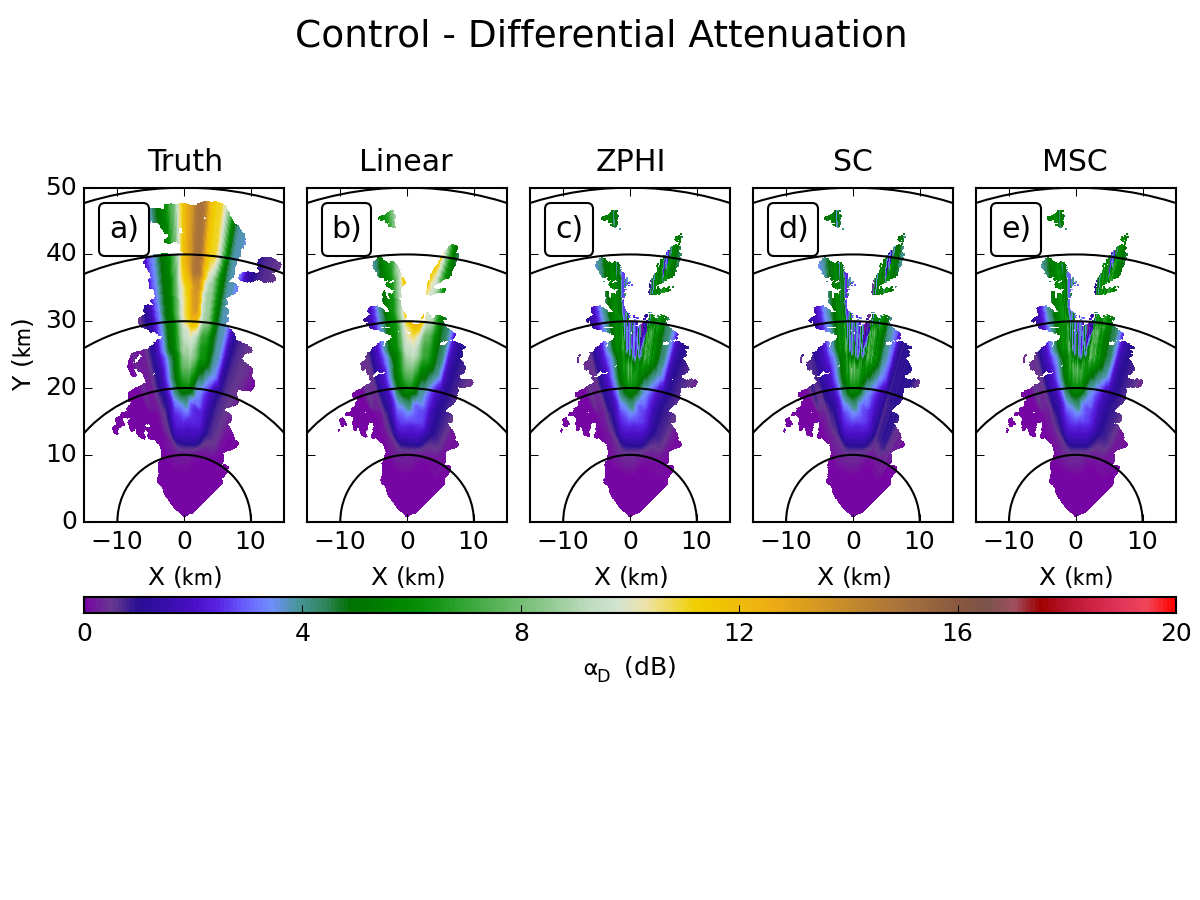
\includegraphics[scale=0.7]{figures/X_Control_Differential_Attenuation}
    \end{center}
\end{frame}

\begin{frame}
    \begin{center}
        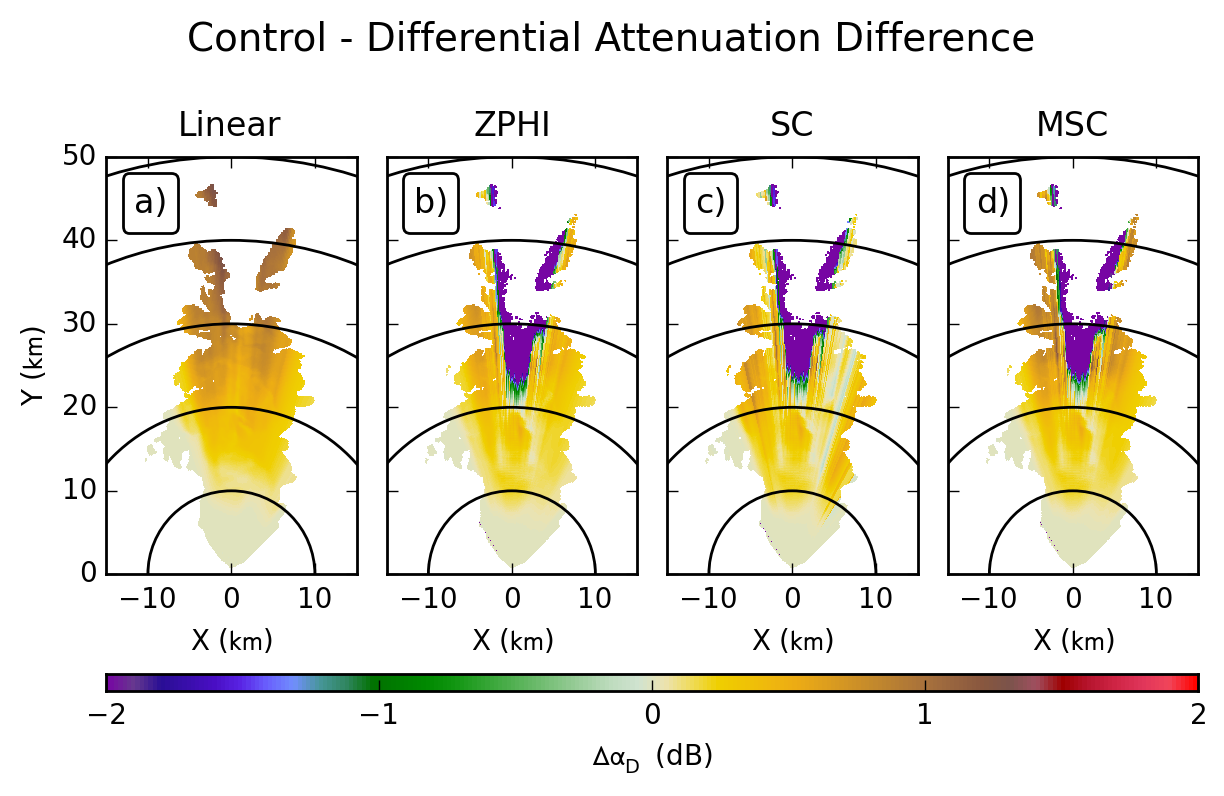
\includegraphics[scale=0.7]{figures/X_Control_Differential_Attenuation_Difference}
    \end{center}
\end{frame}

\begin{frame}
    \begin{center}
        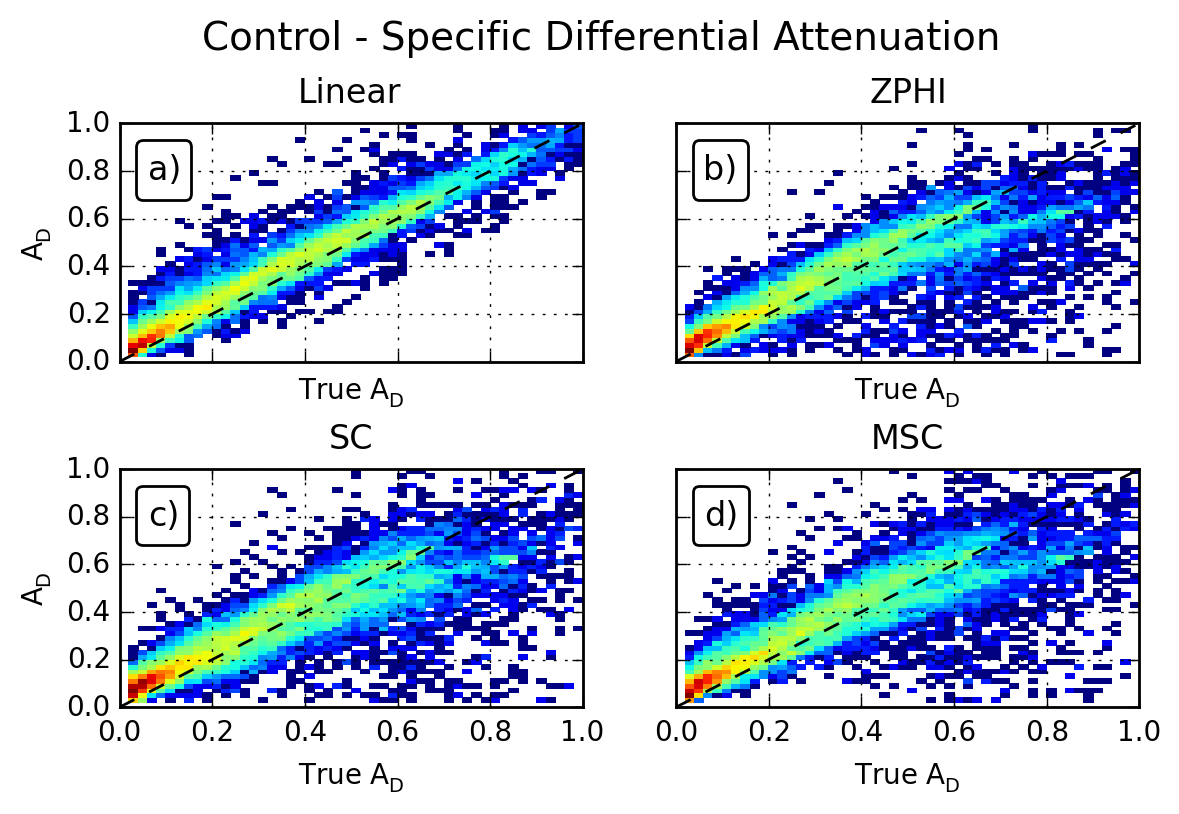
\includegraphics[scale=0.7]{figures/X_Control_Specific_Differential_Attenuation_scatter}
    \end{center}
\end{frame}

\subsubsection{Shape}
\begin{frame}
	\frametitle{Shape}
	\begin{center}
	    \begin{tabular}{ | l | l | }
	        \hline
	        Temperature & \SI{283}{\kelvin} \\
	        Drop Shape Model & Pruppacher \\
	        Wavelength & \SI{5.5}{\centi\meter}, \SI{3.21}{\centi\meter} \\
			\hline
	    \end{tabular}
	\end{center}	
\end{frame}

\begin{frame}
    \begin{center}
        \includegraphics<1>[scale=0.7]{figures/C_Shape_Attenuation_H}
        \includegraphics<2>[scale=0.7]{figures/C_Control_Attenuation_H}
    \end{center}
\end{frame}

\begin{frame}
    \begin{center}
        \includegraphics<1>[scale=0.7]{figures/C_Shape_Attenuation_Difference_H}
        \includegraphics<2>[scale=0.7]{figures/C_Control_Attenuation_Difference_H}
    \end{center}
\end{frame}

\begin{frame}
    \begin{center}
        \includegraphics<1>[scale=0.7]{figures/C_Shape_Specific_Attenuation_H_scatter}
        \includegraphics<2>[scale=0.7]{figures/C_Control_Specific_Attenuation_H_scatter}
    \end{center}
\end{frame}

\begin{frame}
    \begin{center}
        \includegraphics<1>[scale=0.7]{figures/C_Shape_Differential_Attenuation}
        \includegraphics<2>[scale=0.7]{figures/C_Control_Differential_Attenuation}
    \end{center}
\end{frame}

\begin{frame}
    \begin{center}
        \includegraphics<1>[scale=0.7]{figures/C_Shape_Differential_Attenuation_Difference}
        \includegraphics<2>[scale=0.7]{figures/C_Control_Differential_Attenuation_Difference}
    \end{center}
\end{frame}

\begin{frame}
    \begin{center}
        \includegraphics<1>[scale=0.7]{figures/C_Shape_Specific_Differential_Attenuation_scatter}
        \includegraphics<2>[scale=0.7]{figures/C_Control_Specific_Differential_Attenuation_scatter}
    \end{center}
\end{frame}

\begin{frame}
    \begin{center}
        \includegraphics<1>[scale=0.7]{figures/X_Shape_Attenuation_H}
        \includegraphics<2>[scale=0.7]{figures/X_Control_Attenuation_H}
    \end{center}
\end{frame}

\begin{frame}
    \begin{center}
        \includegraphics<1>[scale=0.7]{figures/X_Shape_Attenuation_Difference_H}
        \includegraphics<2>[scale=0.7]{figures/X_Control_Attenuation_Difference_H}
    \end{center}
\end{frame}

\begin{frame}
    \begin{center}
        \includegraphics<1>[scale=0.7]{figures/X_Shape_Specific_Attenuation_H_scatter}
        \includegraphics<2>[scale=0.7]{figures/X_Control_Specific_Attenuation_H_scatter}
    \end{center}
\end{frame}

\begin{frame}
    \begin{center}
        \includegraphics<1>[scale=0.7]{figures/X_Shape_Differential_Attenuation}
        \includegraphics<2>[scale=0.7]{figures/X_Control_Differential_Attenuation}
    \end{center}
\end{frame}

\begin{frame}
    \begin{center}
        \includegraphics<1>[scale=0.7]{figures/X_Shape_Differential_Attenuation_Difference}
        \includegraphics<2>[scale=0.7]{figures/X_Control_Differential_Attenuation_Difference}
    \end{center}
\end{frame}

\begin{frame}
    \begin{center}
        \includegraphics<1>[scale=0.7]{figures/X_Shape_Specific_Differential_Attenuation_scatter}
        \includegraphics<2>[scale=0.7]{figures/X_Control_Specific_Differential_Attenuation_scatter}
    \end{center}
\end{frame}

\subsubsection{Temperature}
\begin{frame}
	\frametitle{Temperature}
	\begin{center}
	    \begin{tabular}{ | l | l | }
	        \hline
	        Temperature & \SI{\~295}{\kelvin} \\
	        Drop Shape Model & Brandes \\
	        Wavelength & \SI{5.5}{\centi\meter}, \SI{3.21}{\centi\meter} \\
			\hline
	    \end{tabular}
	\end{center}	
\end{frame}

\begin{frame}
    \begin{center}
        \includegraphics<1>[scale=0.7]{figures/C_Temperature_Attenuation_H}
        \includegraphics<2>[scale=0.7]{figures/C_Control_Attenuation_H}
    \end{center}
\end{frame}

\begin{frame}
    \begin{center}
        \includegraphics<1>[scale=0.7]{figures/C_Temperature_Attenuation_Difference_H}
        \includegraphics<2>[scale=0.7]{figures/C_Control_Attenuation_Difference_H}
    \end{center}
\end{frame}

\begin{frame}
    \begin{center}
        \includegraphics<1>[scale=0.7]{figures/C_Temperature_Specific_Attenuation_H_scatter}
        \includegraphics<2>[scale=0.7]{figures/C_Control_Specific_Attenuation_H_scatter}
    \end{center}
\end{frame}

\begin{frame}
    \begin{center}
        \includegraphics<1>[scale=0.7]{figures/C_Temperature_Differential_Attenuation}
        \includegraphics<2>[scale=0.7]{figures/C_Control_Differential_Attenuation}
    \end{center}
\end{frame}

\begin{frame}
    \begin{center}
        \includegraphics<1>[scale=0.7]{figures/C_Temperature_Differential_Attenuation_Difference}
        \includegraphics<2>[scale=0.7]{figures/C_Control_Differential_Attenuation_Difference}
    \end{center}
\end{frame}

\begin{frame}
    \begin{center}
        \includegraphics<1>[scale=0.7]{figures/C_Temperature_Specific_Differential_Attenuation_scatter}
        \includegraphics<2>[scale=0.7]{figures/C_Control_Specific_Differential_Attenuation_scatter}
    \end{center}
\end{frame}

\begin{frame}
    \begin{center}
        \includegraphics<1>[scale=0.7]{figures/X_Temperature_Attenuation_H}
        \includegraphics<2>[scale=0.7]{figures/X_Control_Attenuation_H}
    \end{center}
\end{frame}

\begin{frame}
    \begin{center}
        \includegraphics<1>[scale=0.7]{figures/X_Temperature_Attenuation_Difference_H}
        \includegraphics<2>[scale=0.7]{figures/X_Control_Attenuation_Difference_H}
    \end{center}
\end{frame}

\begin{frame}
    \begin{center}
        \includegraphics<1>[scale=0.7]{figures/X_Temperature_Specific_Attenuation_H_scatter}
        \includegraphics<2>[scale=0.7]{figures/X_Control_Specific_Attenuation_H_scatter}
    \end{center}
\end{frame}

\begin{frame}
    \begin{center}
        \includegraphics<1>[scale=0.7]{figures/X_Temperature_Differential_Attenuation}
        \includegraphics<2>[scale=0.7]{figures/X_Control_Differential_Attenuation}
    \end{center}
\end{frame}

\begin{frame}
    \begin{center}
        \includegraphics<1>[scale=0.7]{figures/X_Temperature_Differential_Attenuation_Difference}
        \includegraphics<2>[scale=0.7]{figures/X_Control_Differential_Attenuation_Difference}
    \end{center}
\end{frame}

\begin{frame}
    \begin{center}
        \includegraphics<1>[scale=0.7]{figures/X_Temperature_Specific_Differential_Attenuation_scatter}
        \includegraphics<2>[scale=0.7]{figures/X_Control_Specific_Differential_Attenuation_scatter}
    \end{center}
\end{frame}

\subsubsection{Wavelength}
\begin{frame}
	\frametitle{Control: Matched Assumptions}
	\begin{center}
	    \begin{tabular}{ | l | l | }
	        \hline
	        Temperature & \SI{283}{\kelvin} \\
	        Drop Shape Model & Brandes \\
	        Wavelength & \SI{5.0}{\centi\meter}, \SI{3.0}{\centi\meter} \\
			\hline
	    \end{tabular}
	\end{center}	
\end{frame}
\begin{frame}
    \begin{center}
        \includegraphics<1>[scale=0.7]{figures/C_Wavelength_Attenuation_H}
        \includegraphics<2>[scale=0.7]{figures/C_Control_Attenuation_H}
    \end{center}
\end{frame}

\begin{frame}
    \begin{center}
        \includegraphics<1>[scale=0.7]{figures/C_Wavelength_Attenuation_Difference_H}
        \includegraphics<2>[scale=0.7]{figures/C_Control_Attenuation_Difference_H}
    \end{center}
\end{frame}

\begin{frame}
    \begin{center}
        \includegraphics<1>[scale=0.7]{figures/C_Wavelength_Specific_Attenuation_H_scatter}
        \includegraphics<2>[scale=0.7]{figures/C_Control_Specific_Attenuation_H_scatter}
    \end{center}
\end{frame}

\begin{frame}
    \begin{center}
        \includegraphics<1>[scale=0.7]{figures/C_Wavelength_Differential_Attenuation}
        \includegraphics<2>[scale=0.7]{figures/C_Control_Differential_Attenuation}
    \end{center}
\end{frame}

\begin{frame}
    \begin{center}
        \includegraphics<1>[scale=0.7]{figures/C_Wavelength_Differential_Attenuation_Difference}
        \includegraphics<2>[scale=0.7]{figures/C_Control_Differential_Attenuation_Difference}
    \end{center}
\end{frame}

\begin{frame}
    \begin{center}
        \includegraphics<1>[scale=0.7]{figures/C_Wavelength_Specific_Differential_Attenuation_scatter}
        \includegraphics<2>[scale=0.7]{figures/C_Control_Specific_Differential_Attenuation_scatter}
    \end{center}
\end{frame}

\begin{frame}
    \begin{center}
        \includegraphics<1>[scale=0.7]{figures/X_Wavelength_Attenuation_H}
        \includegraphics<2>[scale=0.7]{figures/X_Control_Attenuation_H}
    \end{center}
\end{frame}

\begin{frame}
    \begin{center}
        \includegraphics<1>[scale=0.7]{figures/X_Wavelength_Attenuation_Difference_H}
        \includegraphics<2>[scale=0.7]{figures/X_Control_Attenuation_Difference_H}
    \end{center}
\end{frame}

\begin{frame}
    \begin{center}
        \includegraphics<1>[scale=0.7]{figures/X_Wavelength_Specific_Attenuation_H_scatter}
        \includegraphics<2>[scale=0.7]{figures/X_Control_Specific_Attenuation_H_scatter}
    \end{center}
\end{frame}

\begin{frame}
    \begin{center}
        \includegraphics<1>[scale=0.7]{figures/X_Wavelength_Differential_Attenuation}
        \includegraphics<2>[scale=0.7]{figures/X_Control_Differential_Attenuation}
    \end{center}
\end{frame}

\begin{frame}
    \begin{center}
        \includegraphics<1>[scale=0.7]{figures/X_Wavelength_Differential_Attenuation_Difference}
        \includegraphics<2>[scale=0.7]{figures/X_Control_Differential_Attenuation_Difference}
    \end{center}
\end{frame}

\begin{frame}
    \begin{center}
        \includegraphics<1>[scale=0.7]{figures/X_Wavelength_Specific_Differential_Attenuation_scatter}
        \includegraphics<2>[scale=0.7]{figures/X_Control_Specific_Differential_Attenuation_scatter}
    \end{center}
\end{frame}

\subsection{Spatial Errors}
\subsubsection{Radial Width}
\begin{frame}
    \begin{center}
        \includegraphics<1>[scale=0.7]{figures/spatial/C_RadialWidth_Attenuation_H}
        \includegraphics<2>[scale=0.7]{figures/spatial/C_Control_Attenuation_H}
    \end{center}
\end{frame}

\begin{frame}
    \begin{center}
        \includegraphics<1>[scale=0.7]{figures/spatial/C_RadialWidth_Attenuation_Difference_H}
        \includegraphics<2>[scale=0.7]{figures/spatial/C_Control_Attenuation_Difference_H}
    \end{center}
\end{frame}

\begin{frame}
    \begin{center}
        \includegraphics<1>[scale=0.7]{figures/spatial/C_RadialWidth_Specific_Attenuation_H_scatter}
        \includegraphics<2>[scale=0.7]{figures/spatial/C_Control_Specific_Attenuation_H_scatter}
    \end{center}
\end{frame}

\begin{frame}
    \begin{center}
        \includegraphics<1>[scale=0.7]{figures/spatial/C_RadialWidth_Differential_Attenuation}
        \includegraphics<2>[scale=0.7]{figures/spatial/C_Control_Differential_Attenuation}
    \end{center}
\end{frame}

\begin{frame}
    \begin{center}
        \includegraphics<1>[scale=0.7]{figures/spatial/C_RadialWidth_Differential_Attenuation_Difference}
        \includegraphics<2>[scale=0.7]{figures/spatial/C_Control_Differential_Attenuation_Difference}
    \end{center}
\end{frame}

\begin{frame}
    \begin{center}
        \includegraphics<1>[scale=0.7]{figures/spatial/C_RadialWidth_Specific_Differential_Attenuation_scatter}
        \includegraphics<2>[scale=0.7]{figures/spatial/C_Control_Specific_Differential_Attenuation_scatter}
    \end{center}
\end{frame}

\begin{frame}
    \begin{center}
        \includegraphics<1>[scale=0.7]{figures/spatial/X_RadialWidth_Attenuation_H}
        \includegraphics<2>[scale=0.7]{figures/spatial/X_Control_Attenuation_H}
    \end{center}
\end{frame}

\begin{frame}
    \begin{center}
        \includegraphics<1>[scale=0.7]{figures/spatial/X_RadialWidth_Attenuation_Difference_H}
        \includegraphics<2>[scale=0.7]{figures/spatial/X_Control_Attenuation_Difference_H}
    \end{center}
\end{frame}

\begin{frame}
    \begin{center}
        \includegraphics<1>[scale=0.7]{figures/spatial/X_RadialWidth_Specific_Attenuation_H_scatter}
        \includegraphics<2>[scale=0.7]{figures/spatial/X_Control_Specific_Attenuation_H_scatter}
    \end{center}
\end{frame}

\begin{frame}
    \begin{center}
        \includegraphics<1>[scale=0.7]{figures/spatial/X_RadialWidth_Differential_Attenuation}
        \includegraphics<2>[scale=0.7]{figures/spatial/X_Control_Differential_Attenuation}
    \end{center}
\end{frame}

\begin{frame}
    \begin{center}
        \includegraphics<1>[scale=0.7]{figures/spatial/X_RadialWidth_Differential_Attenuation_Difference}
        \includegraphics<2>[scale=0.7]{figures/spatial/X_Control_Differential_Attenuation_Difference}
    \end{center}
\end{frame}

\begin{frame}
    \begin{center}
        \includegraphics<1>[scale=0.7]{figures/spatial/X_RadialWidth_Specific_Differential_Attenuation_scatter}
        \includegraphics<2>[scale=0.7]{figures/spatial/X_Control_Specific_Differential_Attenuation_scatter}
    \end{center}
\end{frame}

\subsubsection{Range Resolution}
\begin{frame}
    \begin{center}
        \includegraphics<1>[scale=0.7]{figures/spatial/C_RangeResolution_Attenuation_H}
        \includegraphics<2>[scale=0.7]{figures/spatial/C_Control_Attenuation_H}
    \end{center}
\end{frame}

\begin{frame}
    \begin{center}
        \includegraphics<1>[scale=0.7]{figures/spatial/C_RangeResolution_Attenuation_Difference_H}
        \includegraphics<2>[scale=0.7]{figures/spatial/C_Control_Attenuation_Difference_H}
    \end{center}
\end{frame}

\begin{frame}
    \begin{center}
        \includegraphics<1>[scale=0.7]{figures/spatial/C_RangeResolution_Specific_Attenuation_H_scatter}
        \includegraphics<2>[scale=0.7]{figures/spatial/C_Control_Specific_Attenuation_H_scatter}
    \end{center}
\end{frame}

\begin{frame}
    \begin{center}
        \includegraphics<1>[scale=0.7]{figures/spatial/C_RangeResolution_Differential_Attenuation}
        \includegraphics<2>[scale=0.7]{figures/spatial/C_Control_Differential_Attenuation}
    \end{center}
\end{frame}

\begin{frame}
    \begin{center}
        \includegraphics<1>[scale=0.7]{figures/spatial/C_RangeResolution_Differential_Attenuation_Difference}
        \includegraphics<2>[scale=0.7]{figures/spatial/C_Control_Differential_Attenuation_Difference}
    \end{center}
\end{frame}

\begin{frame}
    \begin{center}
        \includegraphics<1>[scale=0.7]{figures/spatial/C_RangeResolution_Specific_Differential_Attenuation_scatter}
        \includegraphics<2>[scale=0.7]{figures/spatial/C_Control_Specific_Differential_Attenuation_scatter}
    \end{center}
\end{frame}

\begin{frame}
    \begin{center}
        \includegraphics<1>[scale=0.7]{figures/spatial/X_RangeResolution_Attenuation_H}
        \includegraphics<2>[scale=0.7]{figures/spatial/X_Control_Attenuation_H}
    \end{center}
\end{frame}

\begin{frame}
    \begin{center}
        \includegraphics<1>[scale=0.7]{figures/spatial/X_RangeResolution_Attenuation_Difference_H}
        \includegraphics<2>[scale=0.7]{figures/spatial/X_Control_Attenuation_Difference_H}
    \end{center}
\end{frame}

\begin{frame}
    \begin{center}
        \includegraphics<1>[scale=0.7]{figures/spatial/X_RangeResolution_Specific_Attenuation_H_scatter}
        \includegraphics<2>[scale=0.7]{figures/spatial/X_Control_Specific_Attenuation_H_scatter}
    \end{center}
\end{frame}

\begin{frame}
    \begin{center}
        \includegraphics<1>[scale=0.7]{figures/spatial/X_RangeResolution_Differential_Attenuation}
        \includegraphics<2>[scale=0.7]{figures/spatial/X_Control_Differential_Attenuation}
    \end{center}
\end{frame}

\begin{frame}
    \begin{center}
        \includegraphics<1>[scale=0.7]{figures/spatial/X_RangeResolution_Differential_Attenuation_Difference}
        \includegraphics<2>[scale=0.7]{figures/spatial/X_Control_Differential_Attenuation_Difference}
    \end{center}
\end{frame}

\begin{frame}
    \begin{center}
        \includegraphics<1>[scale=0.7]{figures/spatial/X_RangeResolution_Specific_Differential_Attenuation_scatter}
        \includegraphics<2>[scale=0.7]{figures/spatial/X_Control_Specific_Differential_Attenuation_scatter}
    \end{center}
\end{frame}

\subsubsection{Combined}
\begin{frame}
    \begin{center}
        \includegraphics<1>[scale=0.7]{figures/spatial/C_Combined_Attenuation_H}
        \includegraphics<2>[scale=0.7]{figures/spatial/C_Control_Attenuation_H}
    \end{center}
\end{frame}

\begin{frame}
    \begin{center}
        \includegraphics<1>[scale=0.7]{figures/spatial/C_Combined_Attenuation_Difference_H}
        \includegraphics<2>[scale=0.7]{figures/spatial/C_Control_Attenuation_Difference_H}
    \end{center}
\end{frame}

\begin{frame}
    \begin{center}
        \includegraphics<1>[scale=0.7]{figures/spatial/C_Combined_Specific_Attenuation_H_scatter}
        \includegraphics<2>[scale=0.7]{figures/spatial/C_Control_Specific_Attenuation_H_scatter}
    \end{center}
\end{frame}

\begin{frame}
    \begin{center}
        \includegraphics<1>[scale=0.7]{figures/spatial/C_Combined_Differential_Attenuation}
        \includegraphics<2>[scale=0.7]{figures/spatial/C_Control_Differential_Attenuation}
    \end{center}
\end{frame}

\begin{frame}
    \begin{center}
        \includegraphics<1>[scale=0.7]{figures/spatial/C_Combined_Differential_Attenuation_Difference}
        \includegraphics<2>[scale=0.7]{figures/spatial/C_Control_Differential_Attenuation_Difference}
    \end{center}
\end{frame}

\begin{frame}
    \begin{center}
        \includegraphics<1>[scale=0.7]{figures/spatial/C_Combined_Specific_Differential_Attenuation_scatter}
        \includegraphics<2>[scale=0.7]{figures/spatial/C_Control_Specific_Differential_Attenuation_scatter}
    \end{center}
\end{frame}

\begin{frame}
    \begin{center}
        \includegraphics<1>[scale=0.7]{figures/spatial/X_Combined_Attenuation_H}
        \includegraphics<2>[scale=0.7]{figures/spatial/X_Control_Attenuation_H}
    \end{center}
\end{frame}

\begin{frame}
    \begin{center}
        \includegraphics<1>[scale=0.7]{figures/spatial/X_Combined_Attenuation_Difference_H}
        \includegraphics<2>[scale=0.7]{figures/spatial/X_Control_Attenuation_Difference_H}
    \end{center}
\end{frame}

\begin{frame}
    \begin{center}
        \includegraphics<1>[scale=0.7]{figures/spatial/X_Combined_Specific_Attenuation_H_scatter}
        \includegraphics<2>[scale=0.7]{figures/spatial/X_Control_Specific_Attenuation_H_scatter}
    \end{center}
\end{frame}

\begin{frame}
    \begin{center}
        \includegraphics<1>[scale=0.7]{figures/spatial/X_Combined_Differential_Attenuation}
        \includegraphics<2>[scale=0.7]{figures/spatial/X_Control_Differential_Attenuation}
    \end{center}
\end{frame}

\begin{frame}
    \begin{center}
        \includegraphics<1>[scale=0.7]{figures/spatial/X_Combined_Differential_Attenuation_Difference}
        \includegraphics<2>[scale=0.7]{figures/spatial/X_Control_Differential_Attenuation_Difference}
    \end{center}
\end{frame}

\begin{frame}
    \begin{center}
        \includegraphics<1>[scale=0.7]{figures/spatial/X_Combined_Specific_Differential_Attenuation_scatter}
        \includegraphics<2>[scale=0.7]{figures/spatial/X_Control_Specific_Differential_Attenuation_scatter}
    \end{center}
\end{frame}

\section{Conclusion}
\stepcounter{subsection}
\begin{frame}[<+->]
	\frametitle{Conclusions}
	\begin{itemize}
		\item The performance of the linear $\Phi_{DP}$ and ZPHI algorithms depend heavily upon having coefficients
		that reflect the true scattering physics
		\item The self-consistent version of ZPHI performs well overall at removing biases due to changing physics; however this comes
		at a cost of some rays that have increased error
		\item Correction for differential attenuation performs worse across all the algorithms, at least relative to the expected $Z_{DR}$ values
		\item For linear $\Phi_{DP}$ and ZPHI, simply using coefficients to the wave-band of interest can cause non-negligible error
		\item Combining multiple invalid assumptions can actually reduce errors since the biases offset each other
	\end{itemize}
\end{frame}

\begin{frame}
	\frametitle{Thanks}
	\begin{itemize}
		\item Dr. Ted Mansell for performing the model simulation
		\item The NumPy, SciPy, and Matplotlib Python projects that makes this possible
		\item All of my officemates over the years
		\item Dr. Mike Biggerstaff, my advisor, for putting up with me all these years
	\end{itemize}
	\begin{center}
		\large{Questions?}
	\end{center}
\end{frame}

\section{Backup}
\begin{frame}
	\begin{center}
		Backup Slides
	\end{center}
\end{frame}

\subsection{Model Errors}
\subsubsection{Canting}
\begin{frame}
    \begin{center}
        \includegraphics<1>[scale=0.7]{figures/C_Canting_Attenuation_H}
        \includegraphics<2>[scale=0.7]{figures/C_Control_Attenuation_H}
    \end{center}
\end{frame}

\begin{frame}
    \begin{center}
        \includegraphics<1>[scale=0.7]{figures/C_Canting_Attenuation_Difference_H}
        \includegraphics<2>[scale=0.7]{figures/C_Control_Attenuation_Difference_H}
    \end{center}
\end{frame}

\begin{frame}
    \begin{center}
        \includegraphics<1>[scale=0.7]{figures/C_Canting_Specific_Attenuation_H_scatter}
        \includegraphics<2>[scale=0.7]{figures/C_Control_Specific_Attenuation_H_scatter}
    \end{center}
\end{frame}

\begin{frame}
    \begin{center}
        \includegraphics<1>[scale=0.7]{figures/C_Canting_Differential_Attenuation}
        \includegraphics<2>[scale=0.7]{figures/C_Control_Differential_Attenuation}
    \end{center}
\end{frame}

\begin{frame}
    \begin{center}
        \includegraphics<1>[scale=0.7]{figures/C_Canting_Differential_Attenuation_Difference}
        \includegraphics<2>[scale=0.7]{figures/C_Control_Differential_Attenuation_Difference}
    \end{center}
\end{frame}

\begin{frame}
    \begin{center}
        \includegraphics<1>[scale=0.7]{figures/C_Canting_Specific_Differential_Attenuation_scatter}
        \includegraphics<2>[scale=0.7]{figures/C_Control_Specific_Differential_Attenuation_scatter}
    \end{center}
\end{frame}

\begin{frame}
    \begin{center}
        \includegraphics<1>[scale=0.7]{figures/X_Canting_Attenuation_H}
        \includegraphics<2>[scale=0.7]{figures/X_Control_Attenuation_H}
    \end{center}
\end{frame}

\begin{frame}
    \begin{center}
        \includegraphics<1>[scale=0.7]{figures/X_Canting_Attenuation_Difference_H}
        \includegraphics<2>[scale=0.7]{figures/X_Control_Attenuation_Difference_H}
    \end{center}
\end{frame}

\begin{frame}
    \begin{center}
        \includegraphics<1>[scale=0.7]{figures/X_Canting_Specific_Attenuation_H_scatter}
        \includegraphics<2>[scale=0.7]{figures/X_Control_Specific_Attenuation_H_scatter}
    \end{center}
\end{frame}

\begin{frame}
    \begin{center}
        \includegraphics<1>[scale=0.7]{figures/X_Canting_Differential_Attenuation}
        \includegraphics<2>[scale=0.7]{figures/X_Control_Differential_Attenuation}
    \end{center}
\end{frame}

\begin{frame}
    \begin{center}
        \includegraphics<1>[scale=0.7]{figures/X_Canting_Differential_Attenuation_Difference}
        \includegraphics<2>[scale=0.7]{figures/X_Control_Differential_Attenuation_Difference}
    \end{center}
\end{frame}

\begin{frame}
    \begin{center}
        \includegraphics<1>[scale=0.7]{figures/X_Canting_Specific_Differential_Attenuation_scatter}
        \includegraphics<2>[scale=0.7]{figures/X_Control_Specific_Differential_Attenuation_scatter}
    \end{center}
\end{frame}

\subsubsection{Combined}
\begin{frame}
	\frametitle{Worst Case}
	\begin{center}
	    \begin{tabular}{ | l | l | }
	        \hline
	        Temperature & Model Field (\textasciitilde\SI{293}{\kelvin}) \\
	        Drop Shape Model & Pruppacher \\
	        Wavelength & \SI{5.0}{\centi\meter} \\
			\hline
	    \end{tabular}
	\end{center}	
\end{frame}

\begin{frame}
    \begin{center}
        \includegraphics<1>[scale=0.7]{figures/C_Combined_Attenuation_H}
        \includegraphics<2>[scale=0.7]{figures/C_Control_Attenuation_H}
    \end{center}
\end{frame}

\begin{frame}
    \begin{center}
        \includegraphics<1>[scale=0.7]{figures/C_Combined_Attenuation_Difference_H}
        \includegraphics<2>[scale=0.7]{figures/C_Control_Attenuation_Difference_H}
    \end{center}
\end{frame}

\begin{frame}
    \begin{center}
        \includegraphics<1>[scale=0.7]{figures/C_Combined_Specific_Attenuation_H_scatter}
        \includegraphics<2>[scale=0.7]{figures/C_Control_Specific_Attenuation_H_scatter}
    \end{center}
\end{frame}

\begin{frame}
    \begin{center}
        \includegraphics<1>[scale=0.7]{figures/C_Combined_Differential_Attenuation}
        \includegraphics<2>[scale=0.7]{figures/C_Control_Differential_Attenuation}
    \end{center}
\end{frame}

\begin{frame}
    \begin{center}
        \includegraphics<1>[scale=0.7]{figures/C_Combined_Differential_Attenuation_Difference}
        \includegraphics<2>[scale=0.7]{figures/C_Control_Differential_Attenuation_Difference}
    \end{center}
\end{frame}

\begin{frame}
    \begin{center}
        \includegraphics<1>[scale=0.7]{figures/C_Combined_Specific_Differential_Attenuation_scatter}
        \includegraphics<2>[scale=0.7]{figures/C_Control_Specific_Differential_Attenuation_scatter}
    \end{center}
\end{frame}

\begin{frame}
    \begin{center}
        \includegraphics<1>[scale=0.7]{figures/X_Combined_Attenuation_H}
        \includegraphics<2>[scale=0.7]{figures/X_Control_Attenuation_H}
    \end{center}
\end{frame}

\begin{frame}
    \begin{center}
        \includegraphics<1>[scale=0.7]{figures/X_Combined_Attenuation_Difference_H}
        \includegraphics<2>[scale=0.7]{figures/X_Control_Attenuation_Difference_H}
    \end{center}
\end{frame}

\begin{frame}
    \begin{center}
        \includegraphics<1>[scale=0.7]{figures/X_Combined_Specific_Attenuation_H_scatter}
        \includegraphics<2>[scale=0.7]{figures/X_Control_Specific_Attenuation_H_scatter}
    \end{center}
\end{frame}

\begin{frame}
    \begin{center}
        \includegraphics<1>[scale=0.7]{figures/X_Combined_Differential_Attenuation}
        \includegraphics<2>[scale=0.7]{figures/X_Control_Differential_Attenuation}
    \end{center}
\end{frame}

\begin{frame}
    \begin{center}
        \includegraphics<1>[scale=0.7]{figures/X_Combined_Differential_Attenuation_Difference}
        \includegraphics<2>[scale=0.7]{figures/X_Control_Differential_Attenuation_Difference}
    \end{center}
\end{frame}

\begin{frame}
    \begin{center}
        \includegraphics<1>[scale=0.7]{figures/X_Combined_Specific_Differential_Attenuation_scatter}
        \includegraphics<2>[scale=0.7]{figures/X_Control_Specific_Differential_Attenuation_scatter}
    \end{center}
\end{frame}

\subsubsection{Vertical Channel}
\begin{frame}
    \begin{center}
        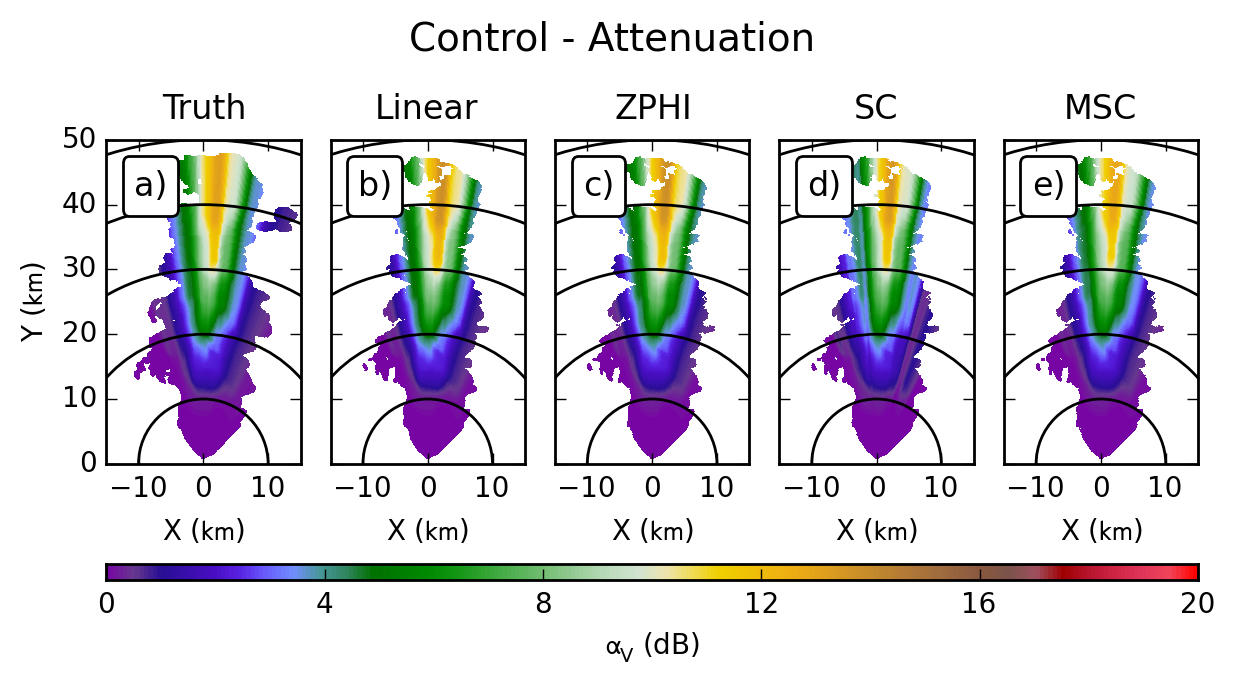
\includegraphics[scale=0.7]{figures/C_Control_Attenuation_V}
    \end{center}
\end{frame}

\begin{frame}
    \begin{center}
        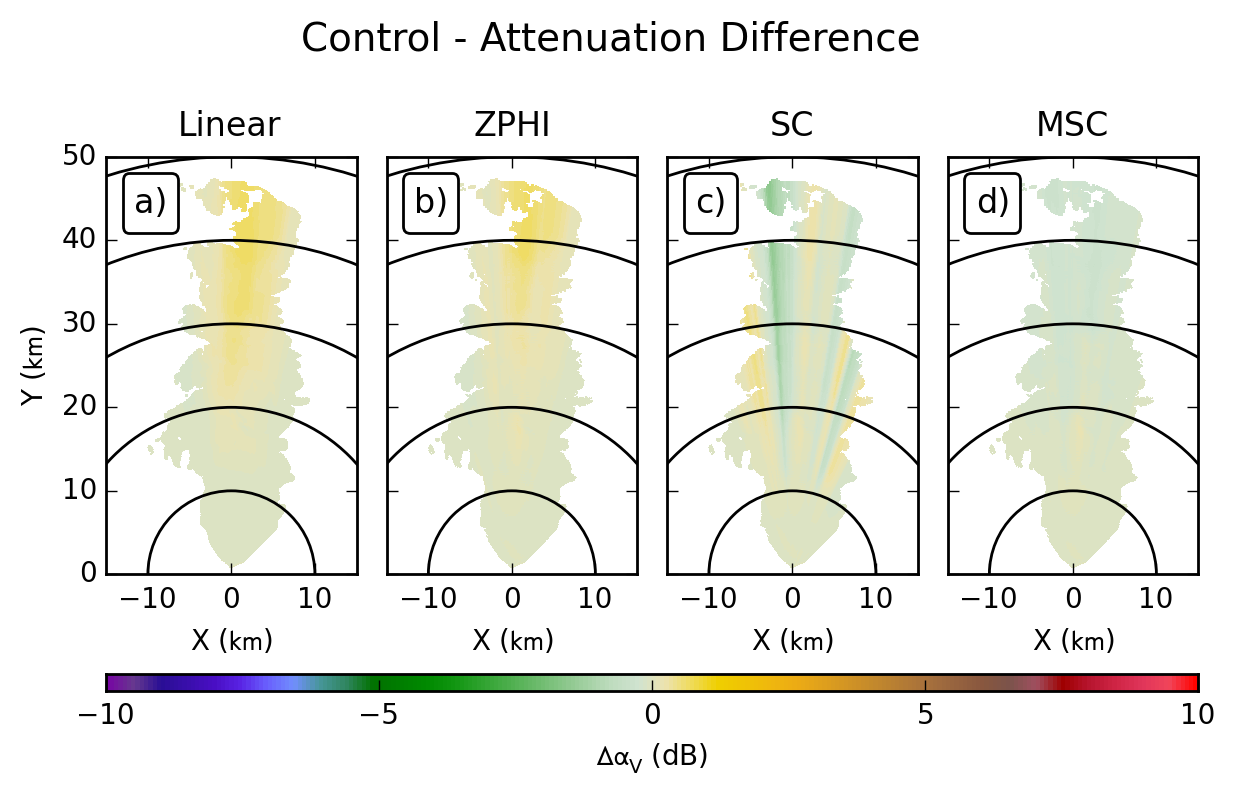
\includegraphics[scale=0.7]{figures/C_Control_Attenuation_Difference_V}
    \end{center}
\end{frame}

\begin{frame}
    \begin{center}
        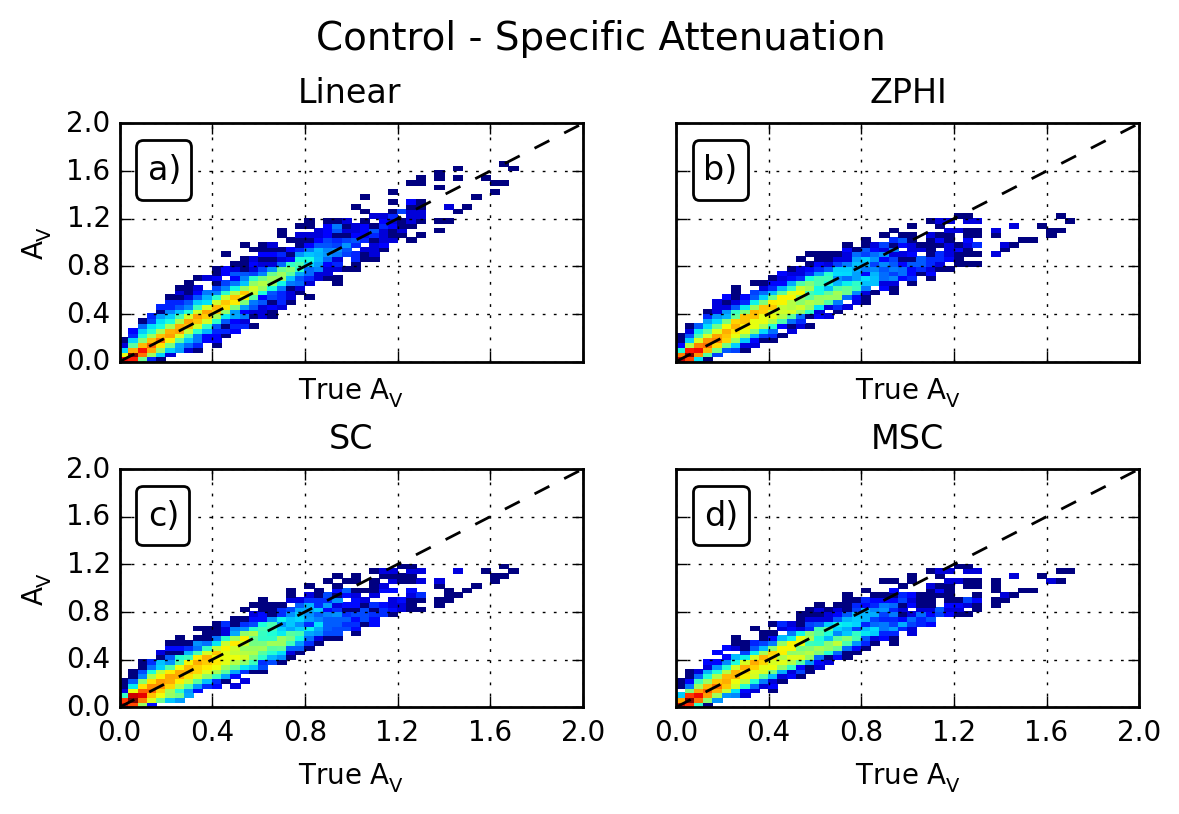
\includegraphics[scale=0.7]{figures/C_Control_Specific_Attenuation_V_scatter}
    \end{center}
\end{frame}

\begin{frame}
    \begin{center}
        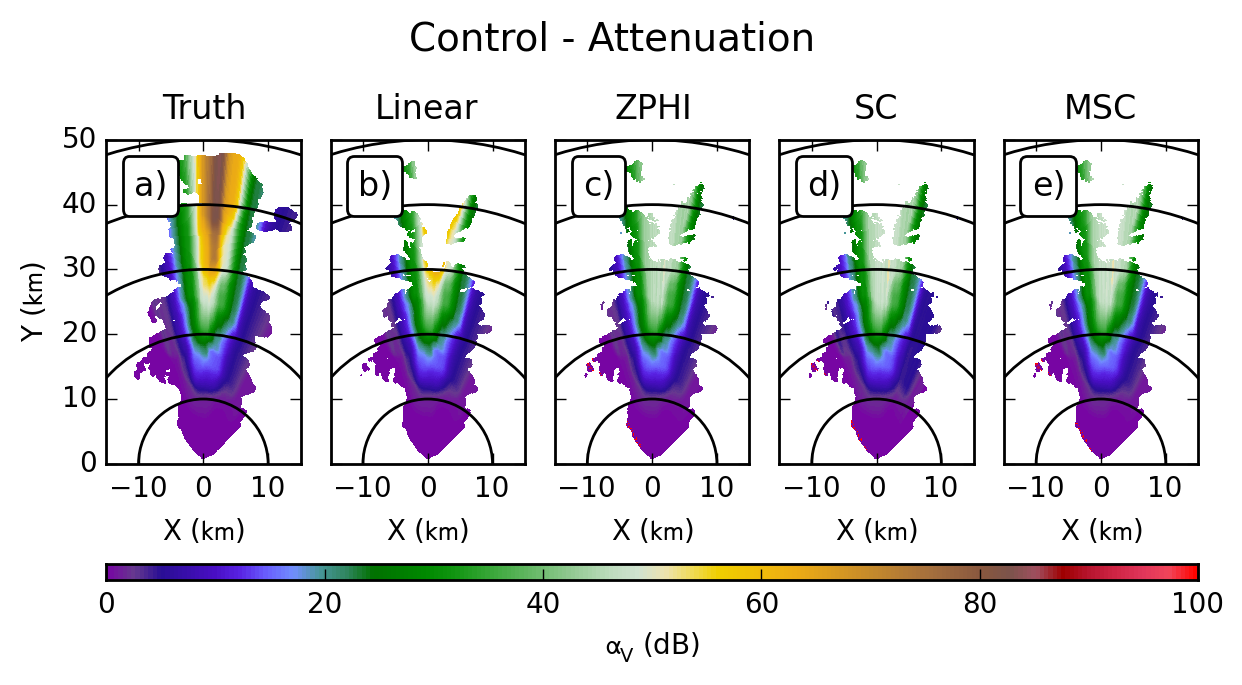
\includegraphics[scale=0.7]{figures/X_Control_Attenuation_V}
    \end{center}
\end{frame}

\begin{frame}
    \begin{center}
        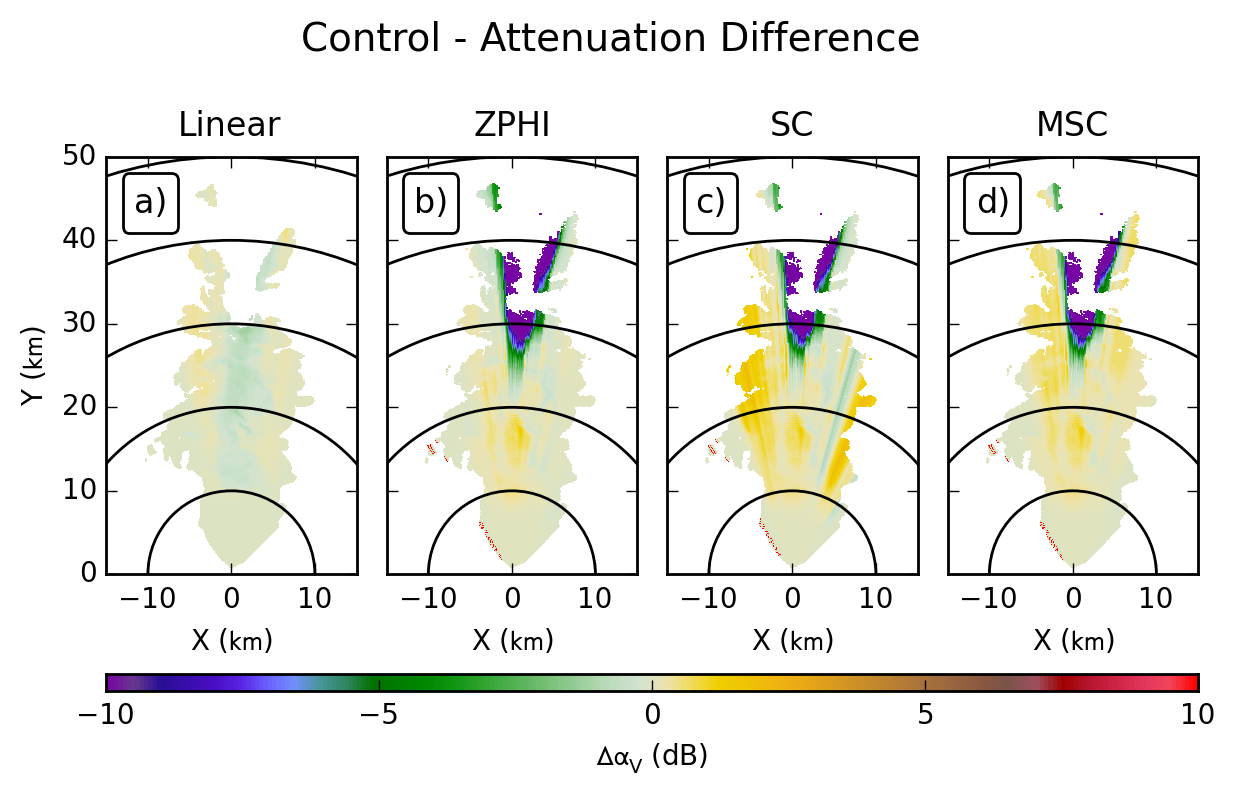
\includegraphics[scale=0.7]{figures/X_Control_Attenuation_Difference_V}
    \end{center}
\end{frame}

\begin{frame}
    \begin{center}
        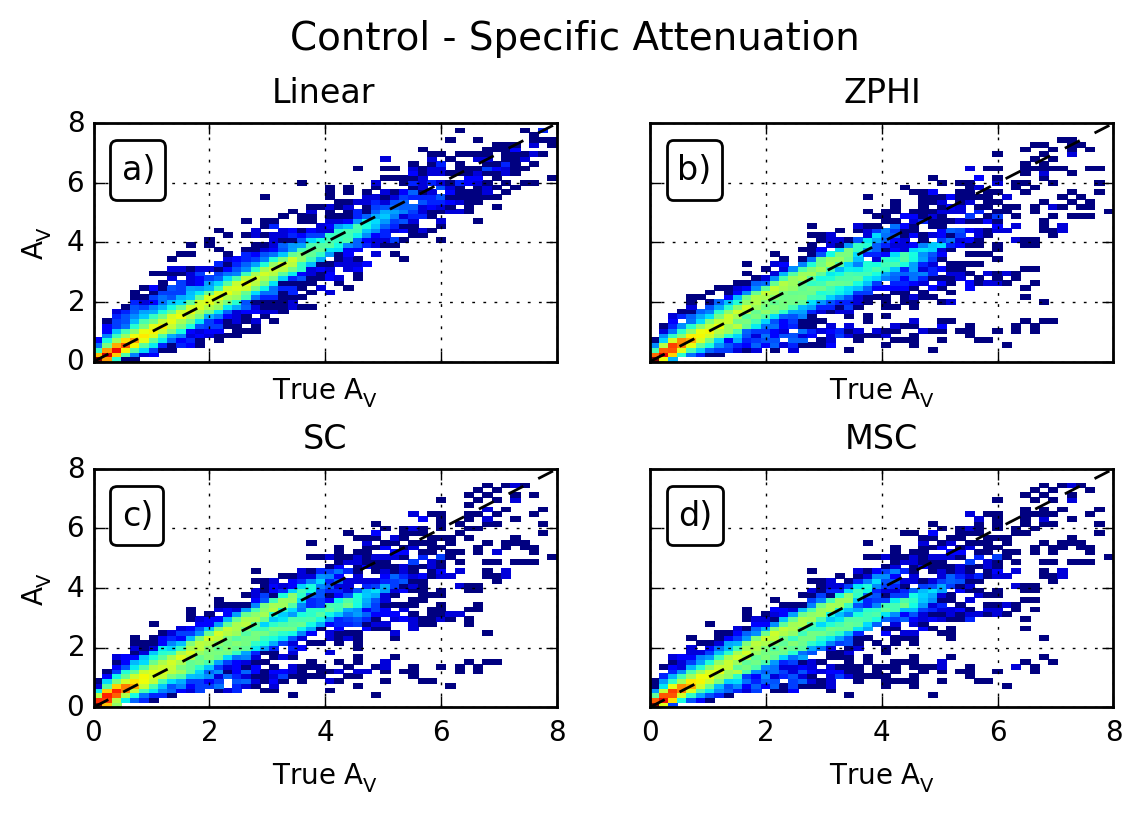
\includegraphics[scale=0.7]{figures/X_Control_Specific_Attenuation_V_scatter}
    \end{center}
\end{frame}

\begin{frame}
    \begin{center}
        \includegraphics<1>[scale=0.7]{figures/C_Canting_Attenuation_V}
        \includegraphics<2>[scale=0.7]{figures/C_Control_Attenuation_V}
    \end{center}
\end{frame}

\begin{frame}
    \begin{center}
        \includegraphics<1>[scale=0.7]{figures/C_Canting_Attenuation_Difference_V}
        \includegraphics<2>[scale=0.7]{figures/C_Control_Attenuation_Difference_V}
    \end{center}
\end{frame}

\begin{frame}
    \begin{center}
        \includegraphics<1>[scale=0.7]{figures/C_Canting_Specific_Attenuation_V_scatter}
        \includegraphics<2>[scale=0.7]{figures/C_Control_Specific_Attenuation_V_scatter}
    \end{center}
\end{frame}

\begin{frame}
    \begin{center}
        \includegraphics<1>[scale=0.7]{figures/X_Canting_Attenuation_V}
        \includegraphics<2>[scale=0.7]{figures/X_Control_Attenuation_V}
    \end{center}
\end{frame}

\begin{frame}
    \begin{center}
        \includegraphics<1>[scale=0.7]{figures/X_Canting_Attenuation_Difference_V}
        \includegraphics<2>[scale=0.7]{figures/X_Control_Attenuation_Difference_V}
    \end{center}
\end{frame}

\begin{frame}
    \begin{center}
        \includegraphics<1>[scale=0.7]{figures/X_Canting_Specific_Attenuation_V_scatter}
        \includegraphics<2>[scale=0.7]{figures/X_Control_Specific_Attenuation_V_scatter}
    \end{center}
\end{frame}

\begin{frame}
    \begin{center}
        \includegraphics<1>[scale=0.7]{figures/C_Shape_Attenuation_V}
        \includegraphics<2>[scale=0.7]{figures/C_Control_Attenuation_V}
    \end{center}
\end{frame}

\begin{frame}
    \begin{center}
        \includegraphics<1>[scale=0.7]{figures/C_Shape_Attenuation_Difference_V}
        \includegraphics<2>[scale=0.7]{figures/C_Control_Attenuation_Difference_V}
    \end{center}
\end{frame}

\begin{frame}
    \begin{center}
        \includegraphics<1>[scale=0.7]{figures/C_Shape_Specific_Attenuation_V_scatter}
        \includegraphics<2>[scale=0.7]{figures/C_Control_Specific_Attenuation_V_scatter}
    \end{center}
\end{frame}

\begin{frame}
    \begin{center}
        \includegraphics<1>[scale=0.7]{figures/X_Shape_Attenuation_V}
        \includegraphics<2>[scale=0.7]{figures/X_Control_Attenuation_V}
    \end{center}
\end{frame}

\begin{frame}
    \begin{center}
        \includegraphics<1>[scale=0.7]{figures/X_Shape_Attenuation_Difference_V}
        \includegraphics<2>[scale=0.7]{figures/X_Control_Attenuation_Difference_V}
    \end{center}
\end{frame}

\begin{frame}
    \begin{center}
        \includegraphics<1>[scale=0.7]{figures/X_Shape_Specific_Attenuation_V_scatter}
        \includegraphics<2>[scale=0.7]{figures/X_Control_Specific_Attenuation_V_scatter}
    \end{center}
\end{frame}

\begin{frame}
    \begin{center}
        \includegraphics<1>[scale=0.7]{figures/C_Temperature_Attenuation_V}
        \includegraphics<2>[scale=0.7]{figures/C_Control_Attenuation_V}
    \end{center}
\end{frame}

\begin{frame}
    \begin{center}
        \includegraphics<1>[scale=0.7]{figures/C_Temperature_Attenuation_Difference_V}
        \includegraphics<2>[scale=0.7]{figures/C_Control_Attenuation_Difference_V}
    \end{center}
\end{frame}

\begin{frame}
    \begin{center}
        \includegraphics<1>[scale=0.7]{figures/C_Temperature_Specific_Attenuation_V_scatter}
        \includegraphics<2>[scale=0.7]{figures/C_Control_Specific_Attenuation_V_scatter}
    \end{center}
\end{frame}

\begin{frame}
    \begin{center}
        \includegraphics<1>[scale=0.7]{figures/X_Temperature_Attenuation_V}
        \includegraphics<2>[scale=0.7]{figures/X_Control_Attenuation_V}
    \end{center}
\end{frame}

\begin{frame}
    \begin{center}
        \includegraphics<1>[scale=0.7]{figures/X_Temperature_Attenuation_Difference_V}
        \includegraphics<2>[scale=0.7]{figures/X_Control_Attenuation_Difference_V}
    \end{center}
\end{frame}

\begin{frame}
    \begin{center}
        \includegraphics<1>[scale=0.7]{figures/X_Temperature_Specific_Attenuation_V_scatter}
        \includegraphics<2>[scale=0.7]{figures/X_Control_Specific_Attenuation_V_scatter}
    \end{center}
\end{frame}

\begin{frame}
    \begin{center}
        \includegraphics<1>[scale=0.7]{figures/C_Wavelength_Attenuation_V}
        \includegraphics<2>[scale=0.7]{figures/C_Control_Attenuation_V}
    \end{center}
\end{frame}

\begin{frame}
    \begin{center}
        \includegraphics<1>[scale=0.7]{figures/C_Wavelength_Attenuation_Difference_V}
        \includegraphics<2>[scale=0.7]{figures/C_Control_Attenuation_Difference_V}
    \end{center}
\end{frame}

\begin{frame}
    \begin{center}
        \includegraphics<1>[scale=0.7]{figures/C_Wavelength_Specific_Attenuation_V_scatter}
        \includegraphics<2>[scale=0.7]{figures/C_Control_Specific_Attenuation_V_scatter}
    \end{center}
\end{frame}

\begin{frame}
    \begin{center}
        \includegraphics<1>[scale=0.7]{figures/X_Wavelength_Attenuation_V}
        \includegraphics<2>[scale=0.7]{figures/X_Control_Attenuation_V}
    \end{center}
\end{frame}

\begin{frame}
    \begin{center}
        \includegraphics<1>[scale=0.7]{figures/X_Wavelength_Attenuation_Difference_V}
        \includegraphics<2>[scale=0.7]{figures/X_Control_Attenuation_Difference_V}
    \end{center}
\end{frame}

\begin{frame}
    \begin{center}
        \includegraphics<1>[scale=0.7]{figures/X_Wavelength_Specific_Attenuation_V_scatter}
        \includegraphics<2>[scale=0.7]{figures/X_Control_Specific_Attenuation_V_scatter}
    \end{center}
\end{frame}

\begin{frame}
    \begin{center}
        \includegraphics<1>[scale=0.7]{figures/C_Combined_Attenuation_V}
        \includegraphics<2>[scale=0.7]{figures/C_Control_Attenuation_V}
    \end{center}
\end{frame}

\begin{frame}
    \begin{center}
        \includegraphics<1>[scale=0.7]{figures/C_Combined_Attenuation_Difference_V}
        \includegraphics<2>[scale=0.7]{figures/C_Control_Attenuation_Difference_V}
    \end{center}
\end{frame}

\begin{frame}
    \begin{center}
        \includegraphics<1>[scale=0.7]{figures/C_Combined_Specific_Attenuation_V_scatter}
        \includegraphics<2>[scale=0.7]{figures/C_Control_Specific_Attenuation_V_scatter}
    \end{center}
\end{frame}

\begin{frame}
    \begin{center}
        \includegraphics<1>[scale=0.7]{figures/X_Combined_Attenuation_V}
        \includegraphics<2>[scale=0.7]{figures/X_Control_Attenuation_V}
    \end{center}
\end{frame}

\begin{frame}
    \begin{center}
        \includegraphics<1>[scale=0.7]{figures/X_Combined_Attenuation_Difference_V}
        \includegraphics<2>[scale=0.7]{figures/X_Control_Attenuation_Difference_V}
    \end{center}
\end{frame}

\begin{frame}
    \begin{center}
        \includegraphics<1>[scale=0.7]{figures/X_Combined_Specific_Attenuation_V_scatter}
        \includegraphics<2>[scale=0.7]{figures/X_Control_Specific_Attenuation_V_scatter}
    \end{center}
\end{frame}

\subsection{Spatial Errors}
\subsubsection{Control}
\begin{frame}
    \begin{center}
        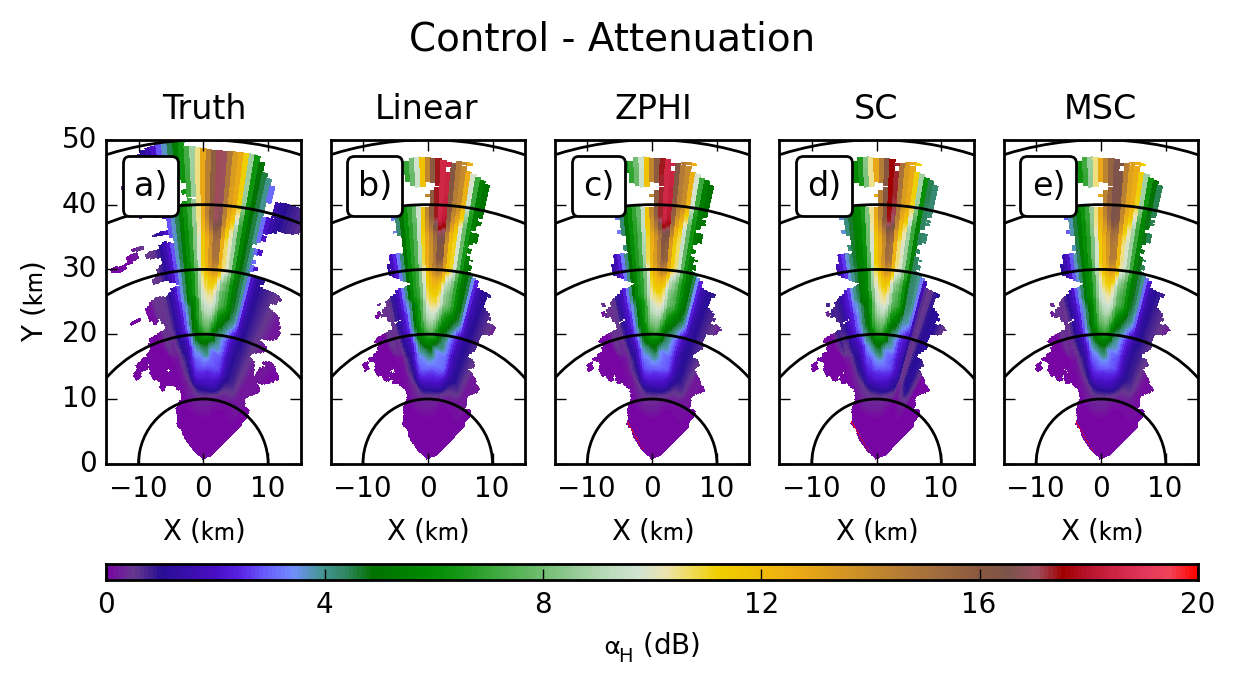
\includegraphics[scale=0.7]{figures/spatial/C_Control_Attenuation_H}
    \end{center}
\end{frame}

\begin{frame}
    \begin{center}
        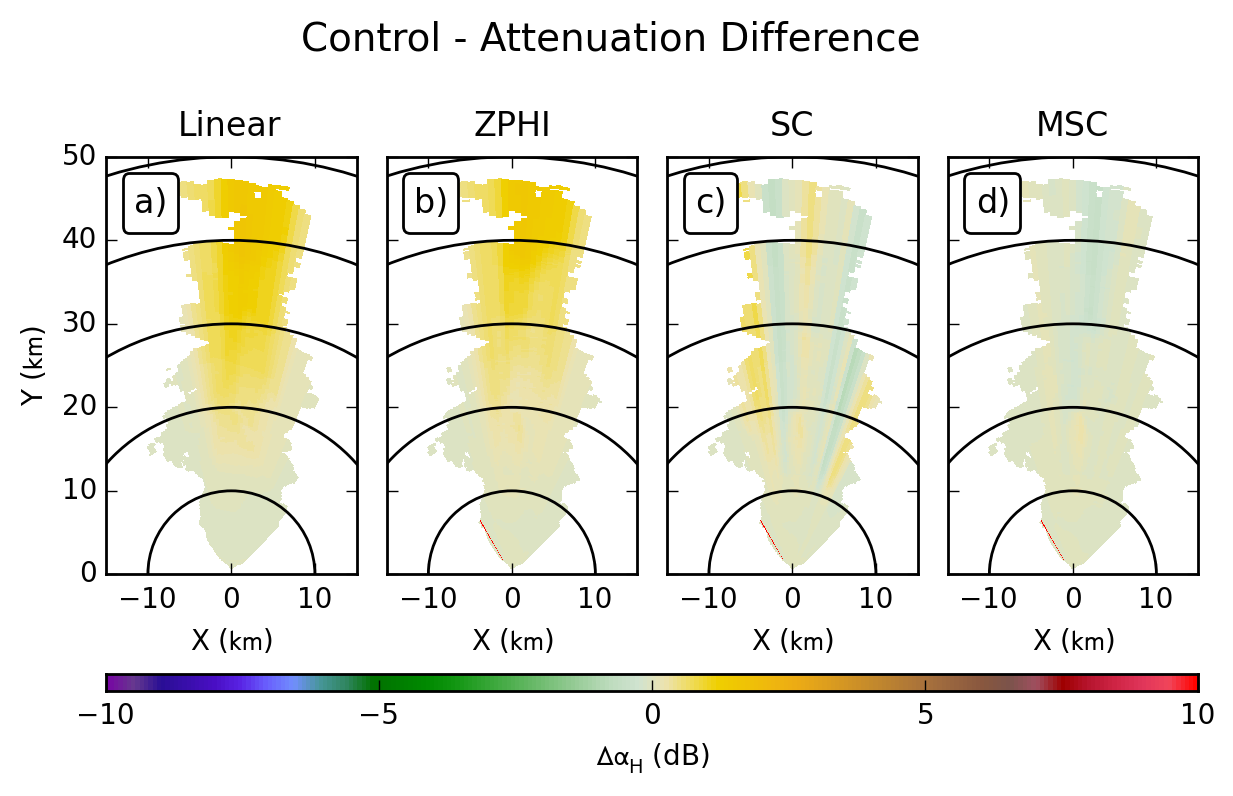
\includegraphics[scale=0.7]{figures/spatial/C_Control_Attenuation_Difference_H}
    \end{center}
\end{frame}

\begin{frame}
    \begin{center}
        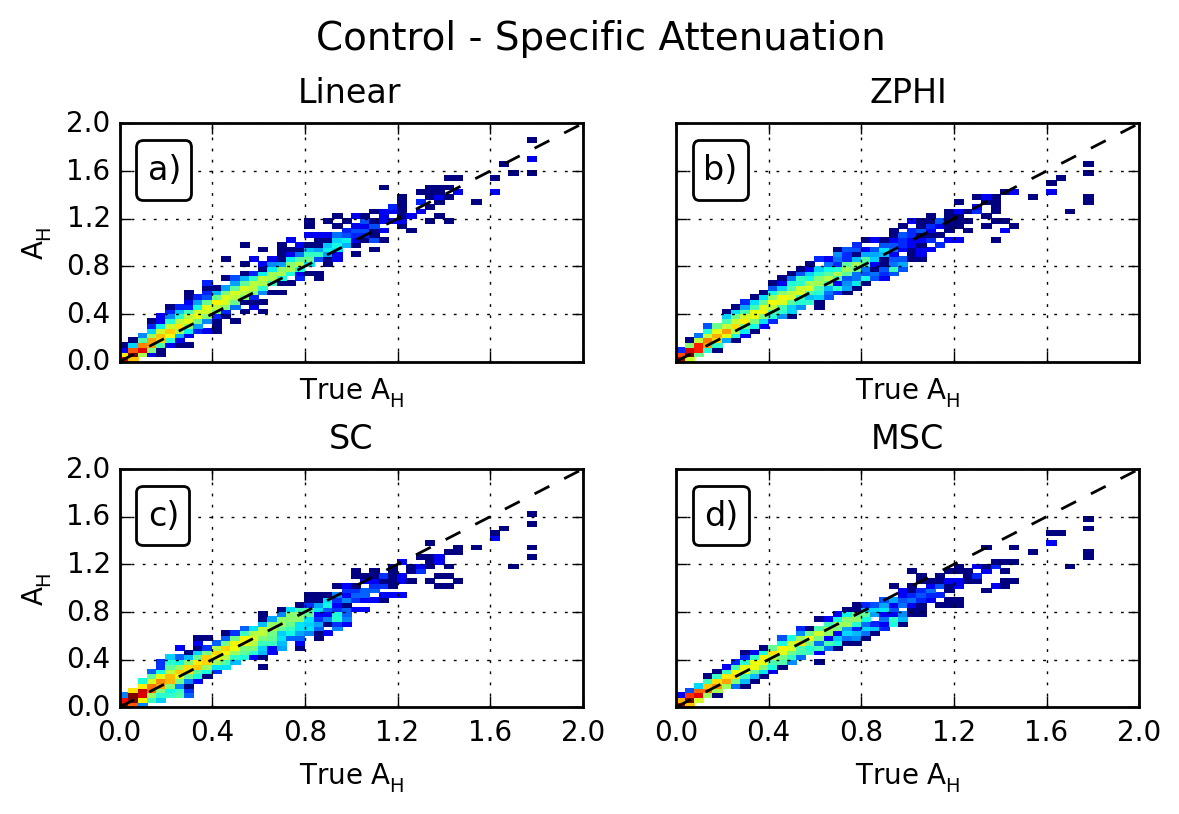
\includegraphics[scale=0.7]{figures/spatial/C_Control_Specific_Attenuation_H_scatter}
    \end{center}
\end{frame}

\begin{frame}
    \begin{center}
        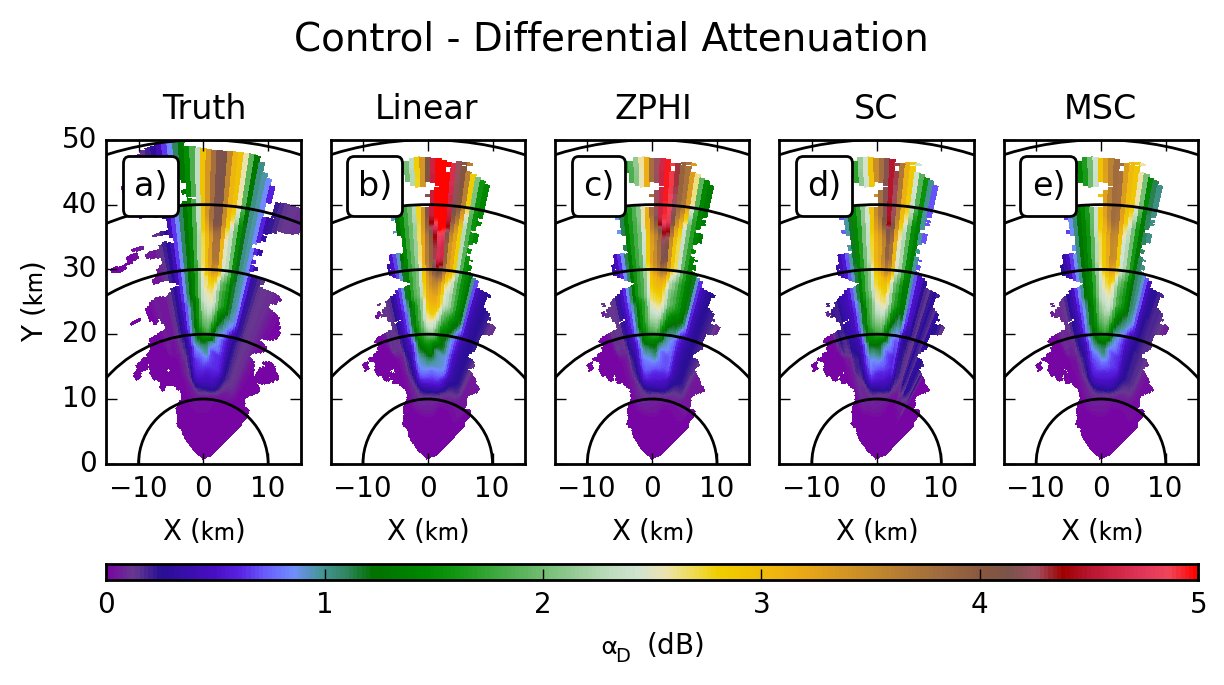
\includegraphics[scale=0.7]{figures/spatial/C_Control_Differential_Attenuation}
    \end{center}
\end{frame}

\begin{frame}
    \begin{center}
        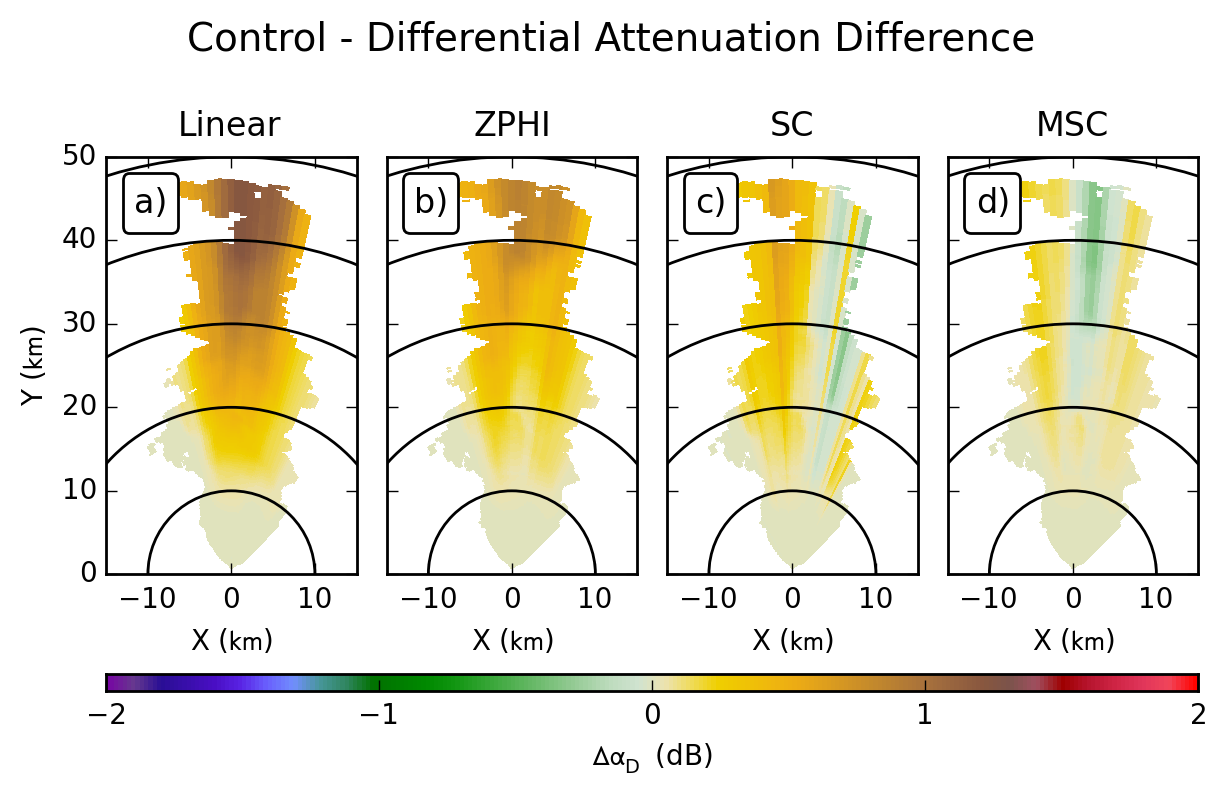
\includegraphics[scale=0.7]{figures/spatial/C_Control_Differential_Attenuation_Difference}
    \end{center}
\end{frame}

\begin{frame}
    \begin{center}
        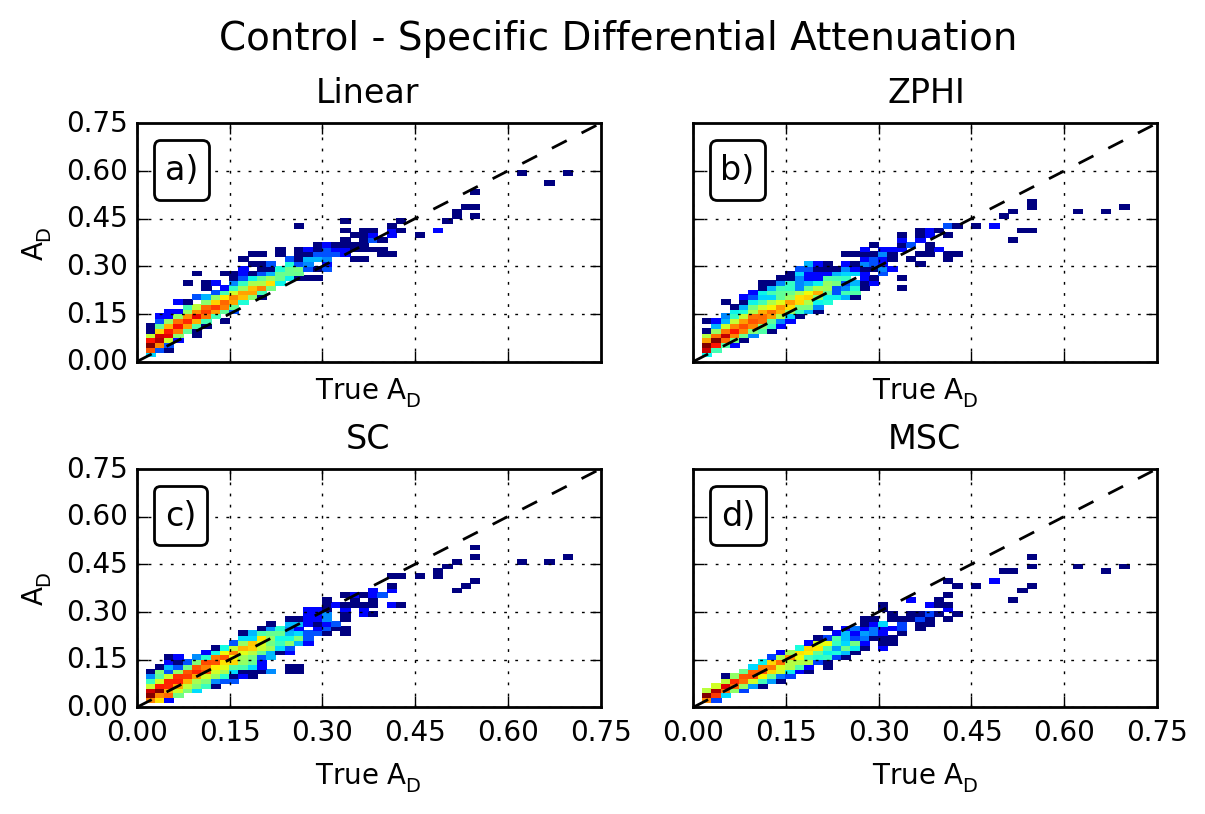
\includegraphics[scale=0.7]{figures/spatial/C_Control_Specific_Differential_Attenuation_scatter}
    \end{center}
\end{frame}

\begin{frame}
    \begin{center}
        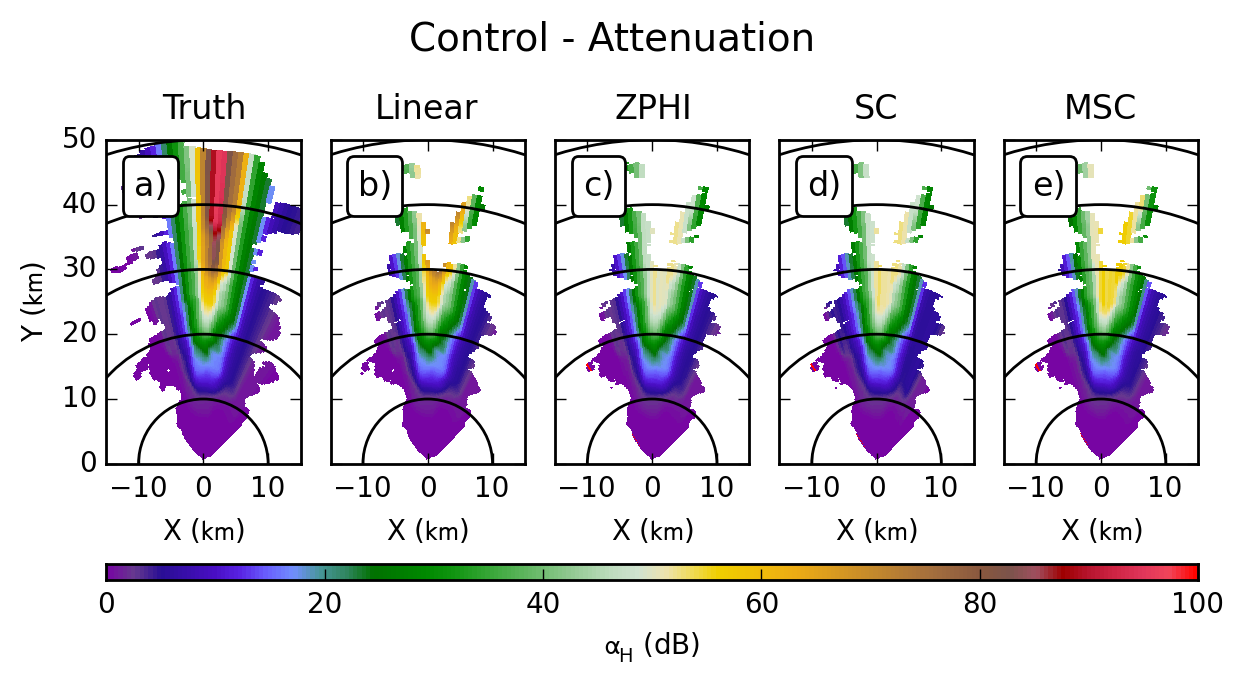
\includegraphics[scale=0.7]{figures/spatial/X_Control_Attenuation_H}
    \end{center}
\end{frame}

\begin{frame}
    \begin{center}
        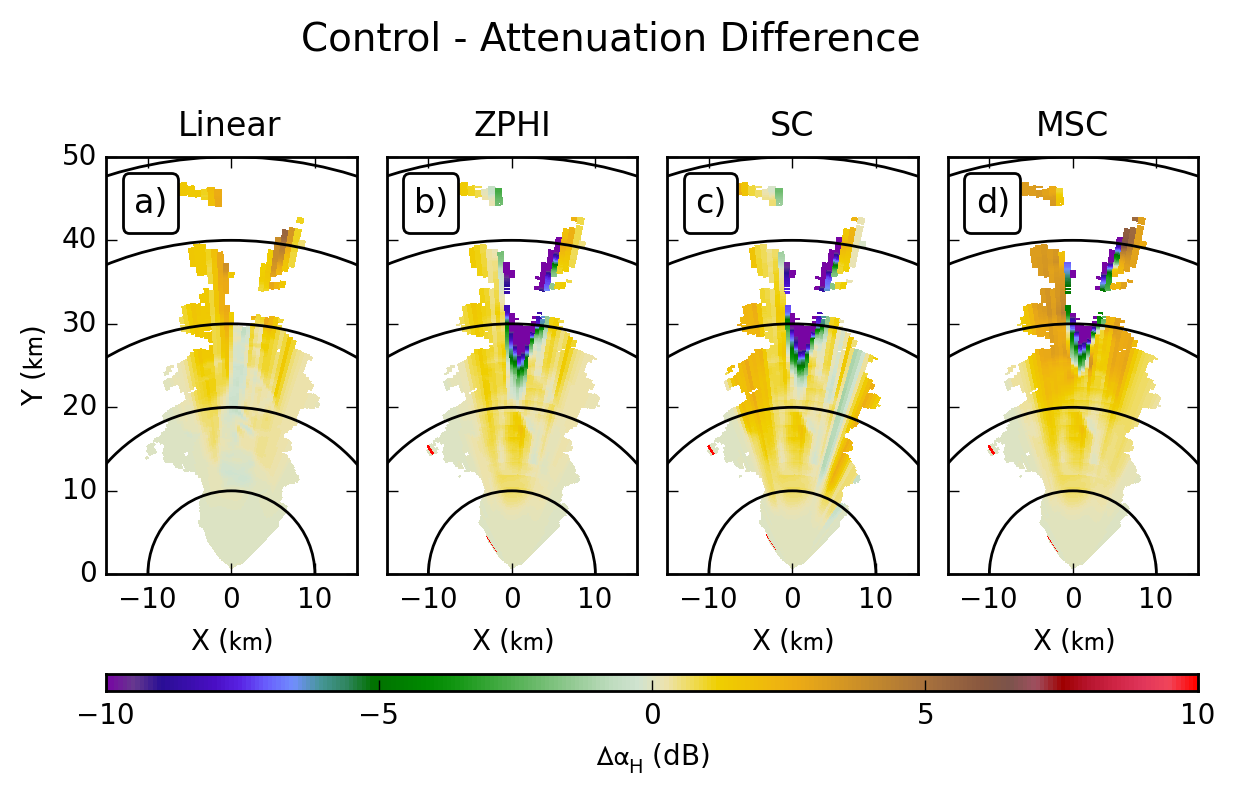
\includegraphics[scale=0.7]{figures/spatial/X_Control_Attenuation_Difference_H}
    \end{center}
\end{frame}

\begin{frame}
    \begin{center}
        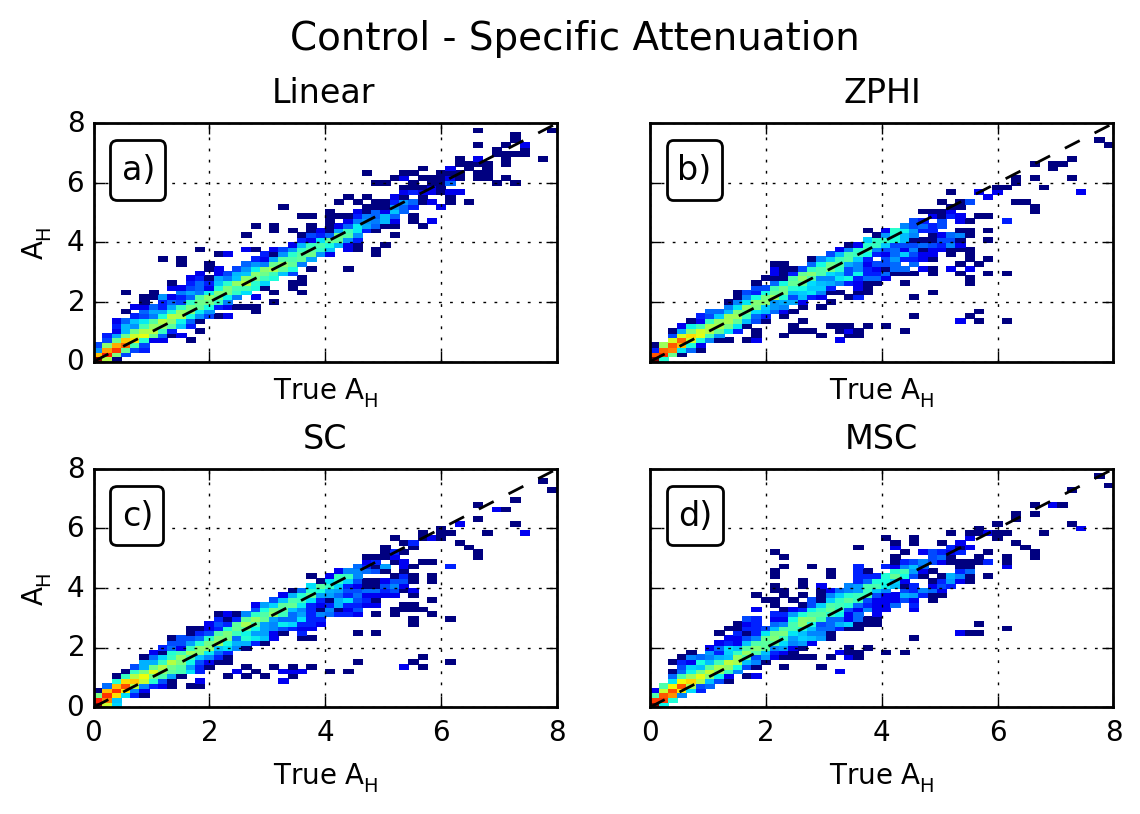
\includegraphics[scale=0.7]{figures/spatial/X_Control_Specific_Attenuation_H_scatter}
    \end{center}
\end{frame}

\begin{frame}
    \begin{center}
        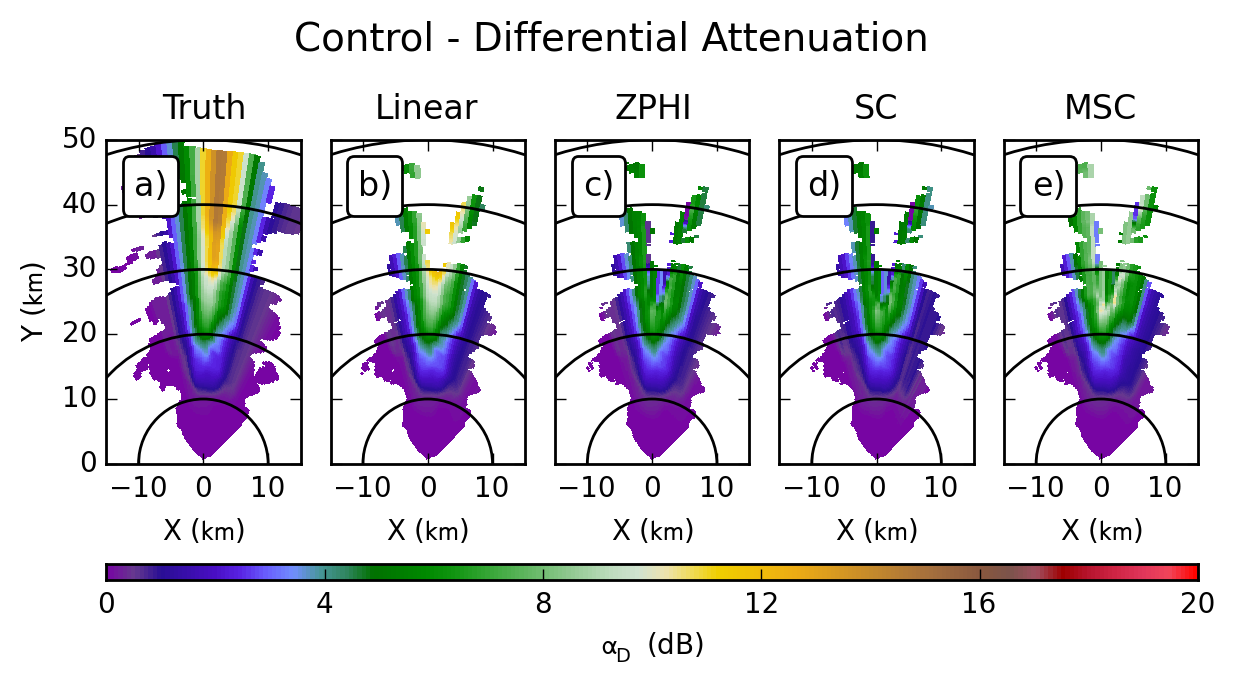
\includegraphics[scale=0.7]{figures/spatial/X_Control_Differential_Attenuation}
    \end{center}
\end{frame}

\begin{frame}
    \begin{center}
        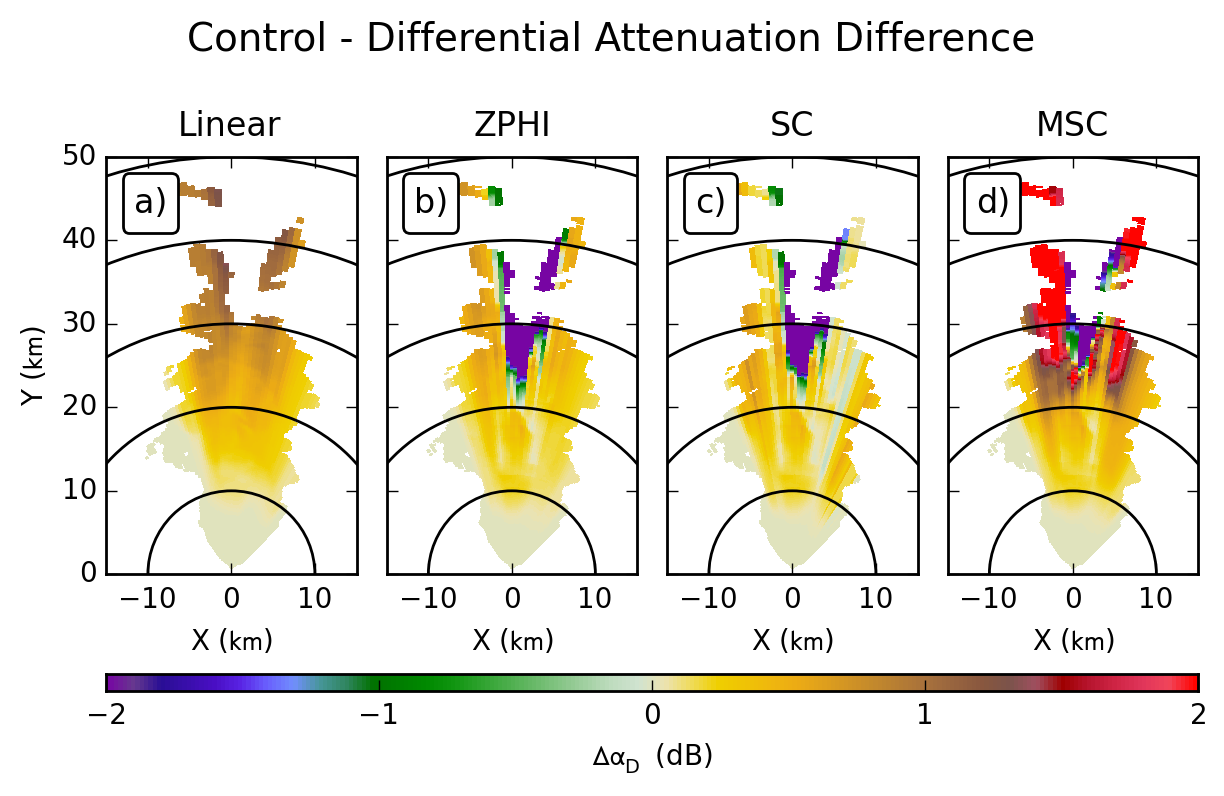
\includegraphics[scale=0.7]{figures/spatial/X_Control_Differential_Attenuation_Difference}
    \end{center}
\end{frame}

\begin{frame}
    \begin{center}
        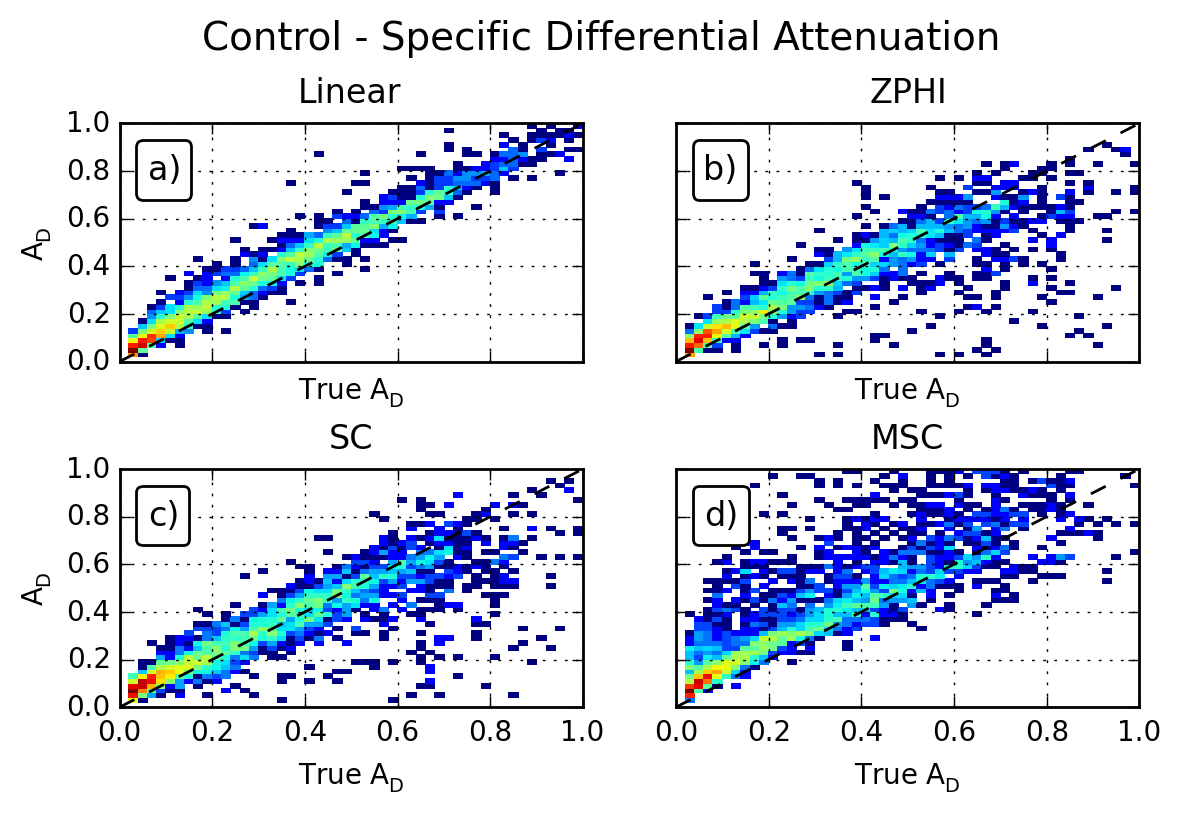
\includegraphics[scale=0.7]{figures/spatial/X_Control_Specific_Differential_Attenuation_scatter}
    \end{center}
\end{frame}

\subsubsection{Sidelobe}
\begin{frame}
    \begin{center}
        \includegraphics<1>[scale=0.7]{figures/spatial/C_Sidelobe_Attenuation_H}
        \includegraphics<2>[scale=0.7]{figures/spatial/C_Control_Attenuation_H}
    \end{center}
\end{frame}

\begin{frame}
    \begin{center}
        \includegraphics<1>[scale=0.7]{figures/spatial/C_Sidelobe_Attenuation_Difference_H}
        \includegraphics<2>[scale=0.7]{figures/spatial/C_Control_Attenuation_Difference_H}
    \end{center}
\end{frame}

\begin{frame}
    \begin{center}
        \includegraphics<1>[scale=0.7]{figures/spatial/C_Sidelobe_Specific_Attenuation_H_scatter}
        \includegraphics<2>[scale=0.7]{figures/spatial/C_Control_Specific_Attenuation_H_scatter}
    \end{center}
\end{frame}

\begin{frame}
    \begin{center}
        \includegraphics<1>[scale=0.7]{figures/spatial/C_Sidelobe_Differential_Attenuation}
        \includegraphics<2>[scale=0.7]{figures/spatial/C_Control_Differential_Attenuation}
    \end{center}
\end{frame}

\begin{frame}
    \begin{center}
        \includegraphics<1>[scale=0.7]{figures/spatial/C_Sidelobe_Differential_Attenuation_Difference}
        \includegraphics<2>[scale=0.7]{figures/spatial/C_Control_Differential_Attenuation_Difference}
    \end{center}
\end{frame}

\begin{frame}
    \begin{center}
        \includegraphics<1>[scale=0.7]{figures/spatial/C_Sidelobe_Specific_Differential_Attenuation_scatter}
        \includegraphics<2>[scale=0.7]{figures/spatial/C_Control_Specific_Differential_Attenuation_scatter}
    \end{center}
\end{frame}

\begin{frame}
    \begin{center}
        \includegraphics<1>[scale=0.7]{figures/spatial/X_Sidelobe_Attenuation_H}
        \includegraphics<2>[scale=0.7]{figures/spatial/X_Control_Attenuation_H}
    \end{center}
\end{frame}

\begin{frame}
    \begin{center}
        \includegraphics<1>[scale=0.7]{figures/spatial/X_Sidelobe_Attenuation_Difference_H}
        \includegraphics<2>[scale=0.7]{figures/spatial/X_Control_Attenuation_Difference_H}
    \end{center}
\end{frame}

\begin{frame}
    \begin{center}
        \includegraphics<1>[scale=0.7]{figures/spatial/X_Sidelobe_Specific_Attenuation_H_scatter}
        \includegraphics<2>[scale=0.7]{figures/spatial/X_Control_Specific_Attenuation_H_scatter}
    \end{center}
\end{frame}

\begin{frame}
    \begin{center}
        \includegraphics<1>[scale=0.7]{figures/spatial/X_Sidelobe_Differential_Attenuation}
        \includegraphics<2>[scale=0.7]{figures/spatial/X_Control_Differential_Attenuation}
    \end{center}
\end{frame}

\begin{frame}
    \begin{center}
        \includegraphics<1>[scale=0.7]{figures/spatial/X_Sidelobe_Differential_Attenuation_Difference}
        \includegraphics<2>[scale=0.7]{figures/spatial/X_Control_Differential_Attenuation_Difference}
    \end{center}
\end{frame}

\begin{frame}
    \begin{center}
        \includegraphics<1>[scale=0.7]{figures/spatial/X_Sidelobe_Specific_Differential_Attenuation_scatter}
        \includegraphics<2>[scale=0.7]{figures/spatial/X_Control_Specific_Differential_Attenuation_scatter}
    \end{center}
\end{frame}

\subsubsection{Beamwidth}
\begin{frame}
    \begin{center}
        \includegraphics<1>[scale=0.7]{figures/spatial/C_Beamwidth_Attenuation_H}
        \includegraphics<2>[scale=0.7]{figures/spatial/C_Control_Attenuation_H}
    \end{center}
\end{frame}

\begin{frame}
    \begin{center}
        \includegraphics<1>[scale=0.7]{figures/spatial/C_Beamwidth_Attenuation_Difference_H}
        \includegraphics<2>[scale=0.7]{figures/spatial/C_Control_Attenuation_Difference_H}
    \end{center}
\end{frame}

\begin{frame}
    \begin{center}
        \includegraphics<1>[scale=0.7]{figures/spatial/C_Beamwidth_Specific_Attenuation_H_scatter}
        \includegraphics<2>[scale=0.7]{figures/spatial/C_Control_Specific_Attenuation_H_scatter}
    \end{center}
\end{frame}

\begin{frame}
    \begin{center}
        \includegraphics<1>[scale=0.7]{figures/spatial/C_Beamwidth_Differential_Attenuation}
        \includegraphics<2>[scale=0.7]{figures/spatial/C_Control_Differential_Attenuation}
    \end{center}
\end{frame}

\begin{frame}
    \begin{center}
        \includegraphics<1>[scale=0.7]{figures/spatial/C_Beamwidth_Differential_Attenuation_Difference}
        \includegraphics<2>[scale=0.7]{figures/spatial/C_Control_Differential_Attenuation_Difference}
    \end{center}
\end{frame}

\begin{frame}
    \begin{center}
        \includegraphics<1>[scale=0.7]{figures/spatial/C_Beamwidth_Specific_Differential_Attenuation_scatter}
        \includegraphics<2>[scale=0.7]{figures/spatial/C_Control_Specific_Differential_Attenuation_scatter}
    \end{center}
\end{frame}

\begin{frame}
    \begin{center}
        \includegraphics<1>[scale=0.7]{figures/spatial/X_Beamwidth_Attenuation_H}
        \includegraphics<2>[scale=0.7]{figures/spatial/X_Control_Attenuation_H}
    \end{center}
\end{frame}

\begin{frame}
    \begin{center}
        \includegraphics<1>[scale=0.7]{figures/spatial/X_Beamwidth_Attenuation_Difference_H}
        \includegraphics<2>[scale=0.7]{figures/spatial/X_Control_Attenuation_Difference_H}
    \end{center}
\end{frame}

\begin{frame}
    \begin{center}
        \includegraphics<1>[scale=0.7]{figures/spatial/X_Beamwidth_Specific_Attenuation_H_scatter}
        \includegraphics<2>[scale=0.7]{figures/spatial/X_Control_Specific_Attenuation_H_scatter}
    \end{center}
\end{frame}

\begin{frame}
    \begin{center}
        \includegraphics<1>[scale=0.7]{figures/spatial/X_Beamwidth_Differential_Attenuation}
        \includegraphics<2>[scale=0.7]{figures/spatial/X_Control_Differential_Attenuation}
    \end{center}
\end{frame}

\begin{frame}
    \begin{center}
        \includegraphics<1>[scale=0.7]{figures/spatial/X_Beamwidth_Differential_Attenuation_Difference}
        \includegraphics<2>[scale=0.7]{figures/spatial/X_Control_Differential_Attenuation_Difference}
    \end{center}
\end{frame}

\begin{frame}
    \begin{center}
        \includegraphics<1>[scale=0.7]{figures/spatial/X_Beamwidth_Specific_Differential_Attenuation_scatter}
        \includegraphics<2>[scale=0.7]{figures/spatial/X_Control_Specific_Differential_Attenuation_scatter}
    \end{center}
\end{frame}

\subsubsection{Vertical Channel}
\begin{frame}
    \begin{center}
        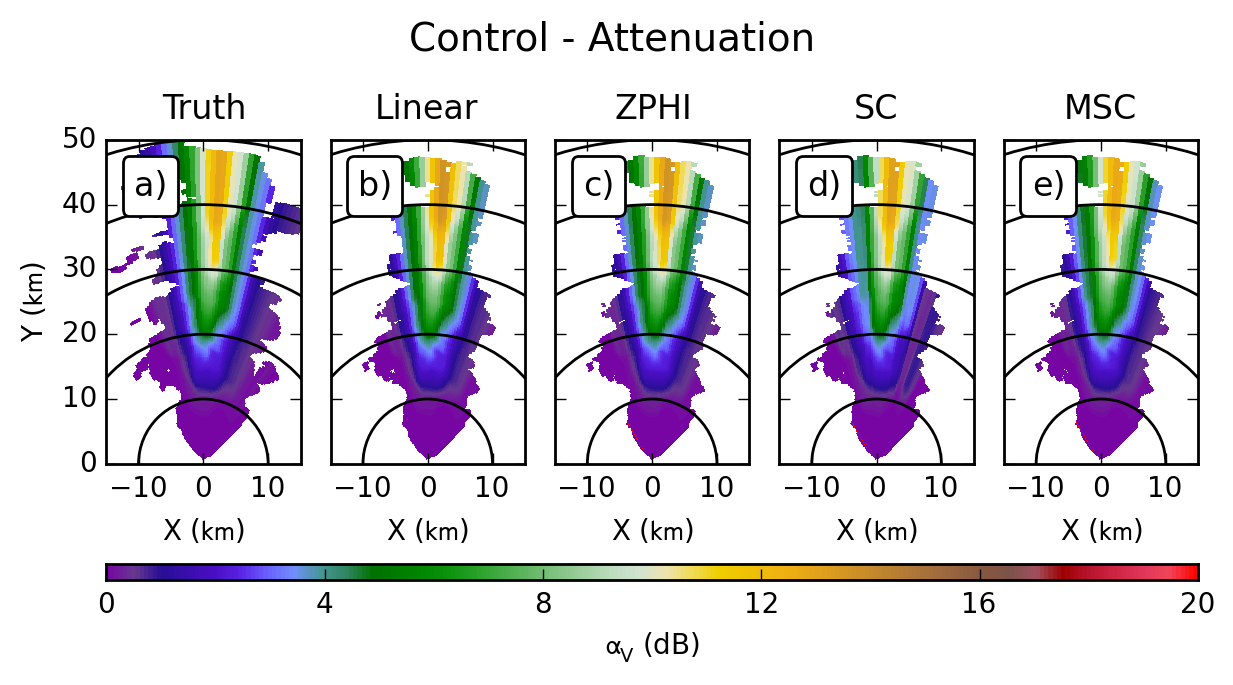
\includegraphics[scale=0.7]{figures/spatial/C_Control_Attenuation_V}
    \end{center}
\end{frame}

\begin{frame}
    \begin{center}
        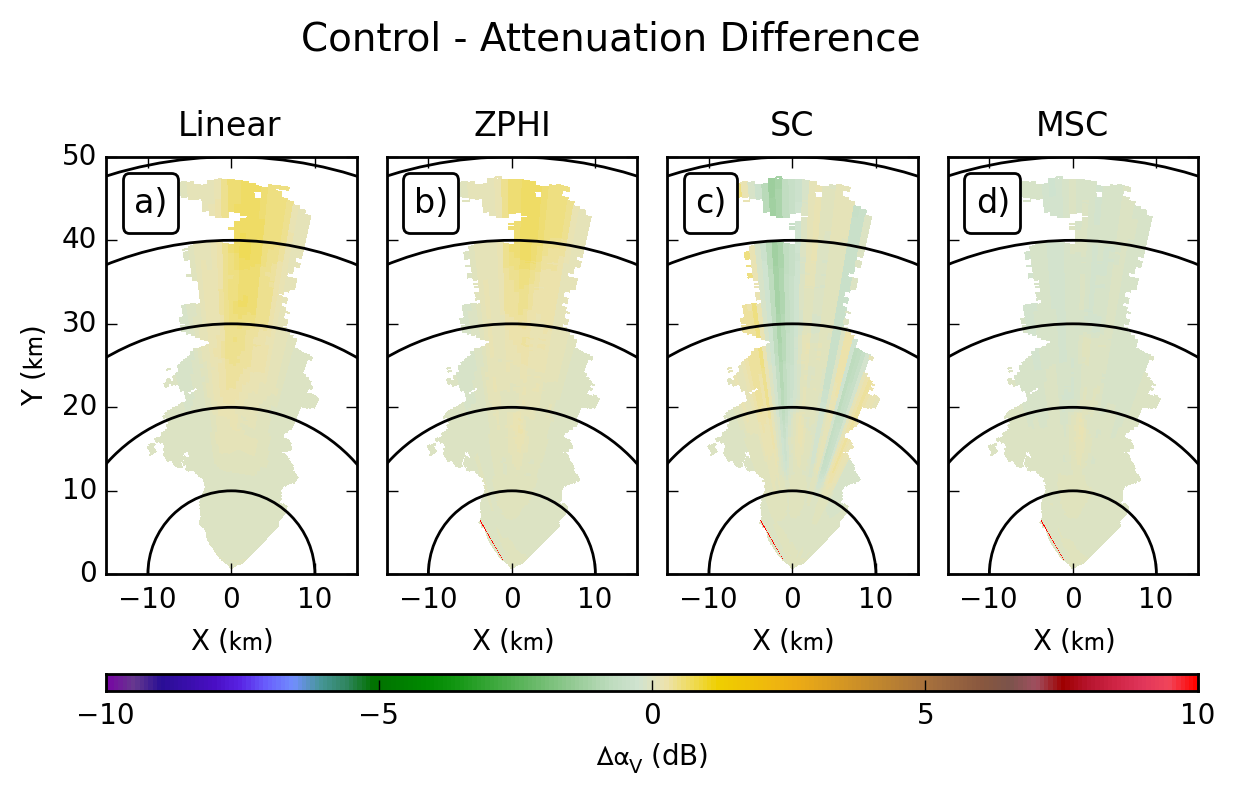
\includegraphics[scale=0.7]{figures/spatial/C_Control_Attenuation_Difference_V}
    \end{center}
\end{frame}

\begin{frame}
    \begin{center}
        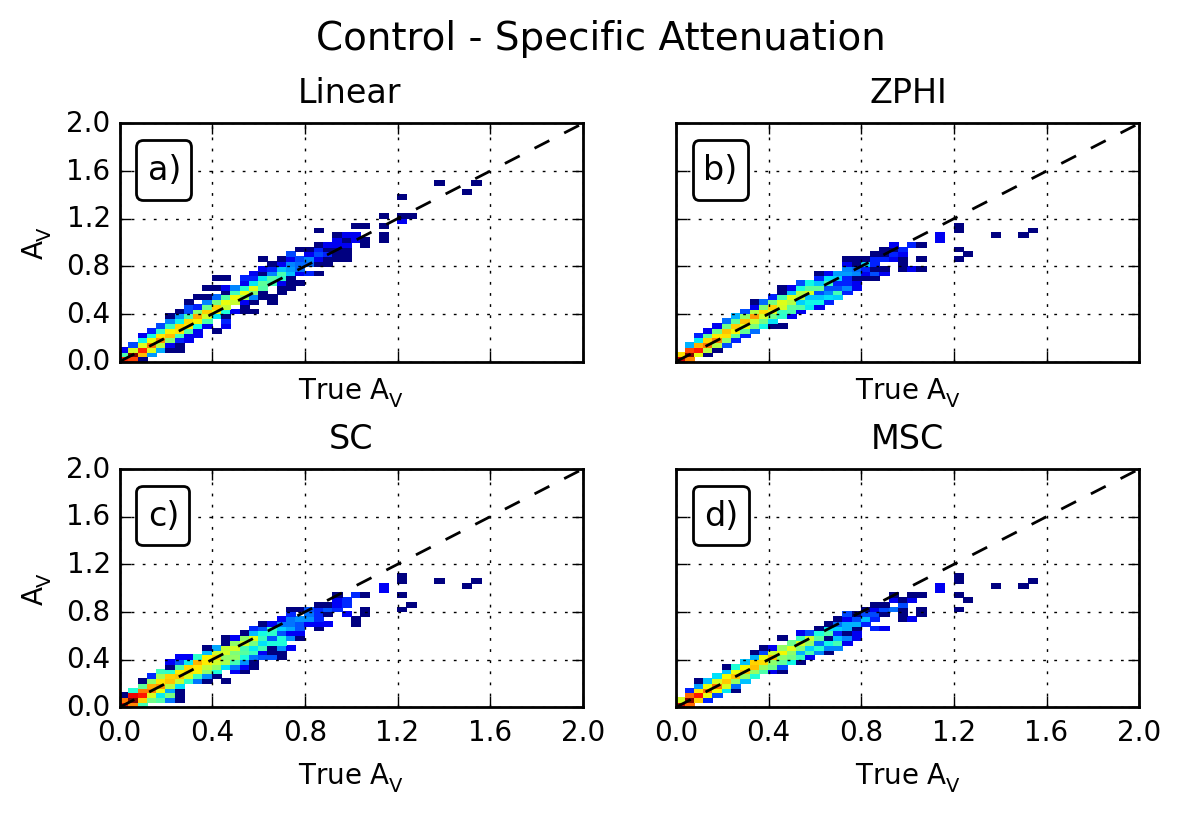
\includegraphics[scale=0.7]{figures/spatial/C_Control_Specific_Attenuation_V_scatter}
    \end{center}
\end{frame}

\begin{frame}
    \begin{center}
        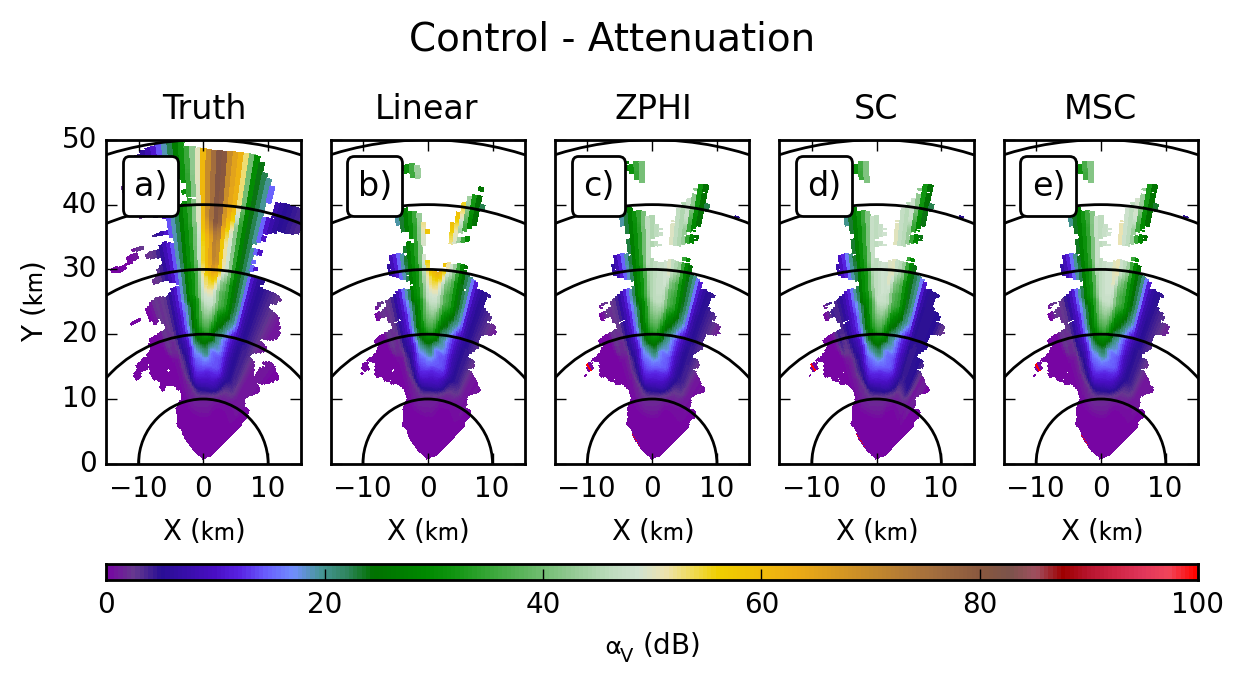
\includegraphics[scale=0.7]{figures/spatial/X_Control_Attenuation_V}
    \end{center}
\end{frame}

\begin{frame}
    \begin{center}
        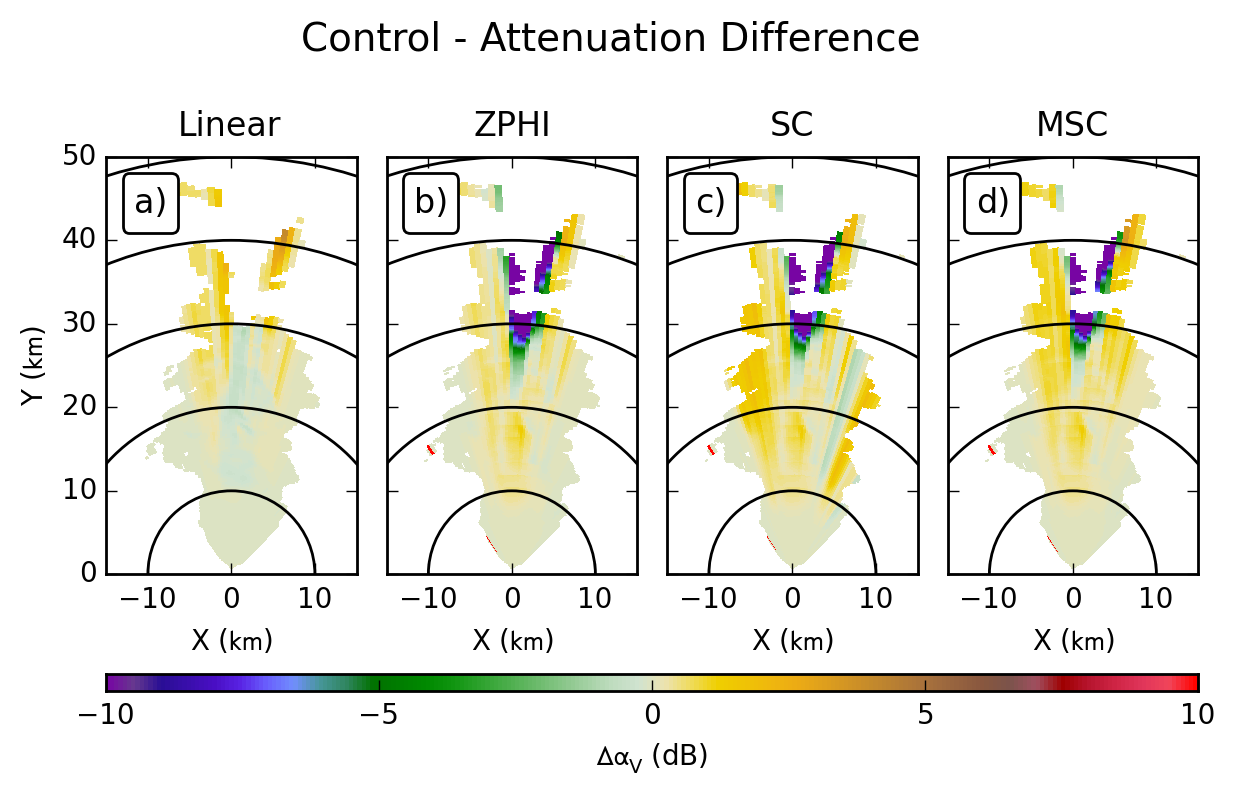
\includegraphics[scale=0.7]{figures/spatial/X_Control_Attenuation_Difference_V}
    \end{center}
\end{frame}

\begin{frame}
    \begin{center}
        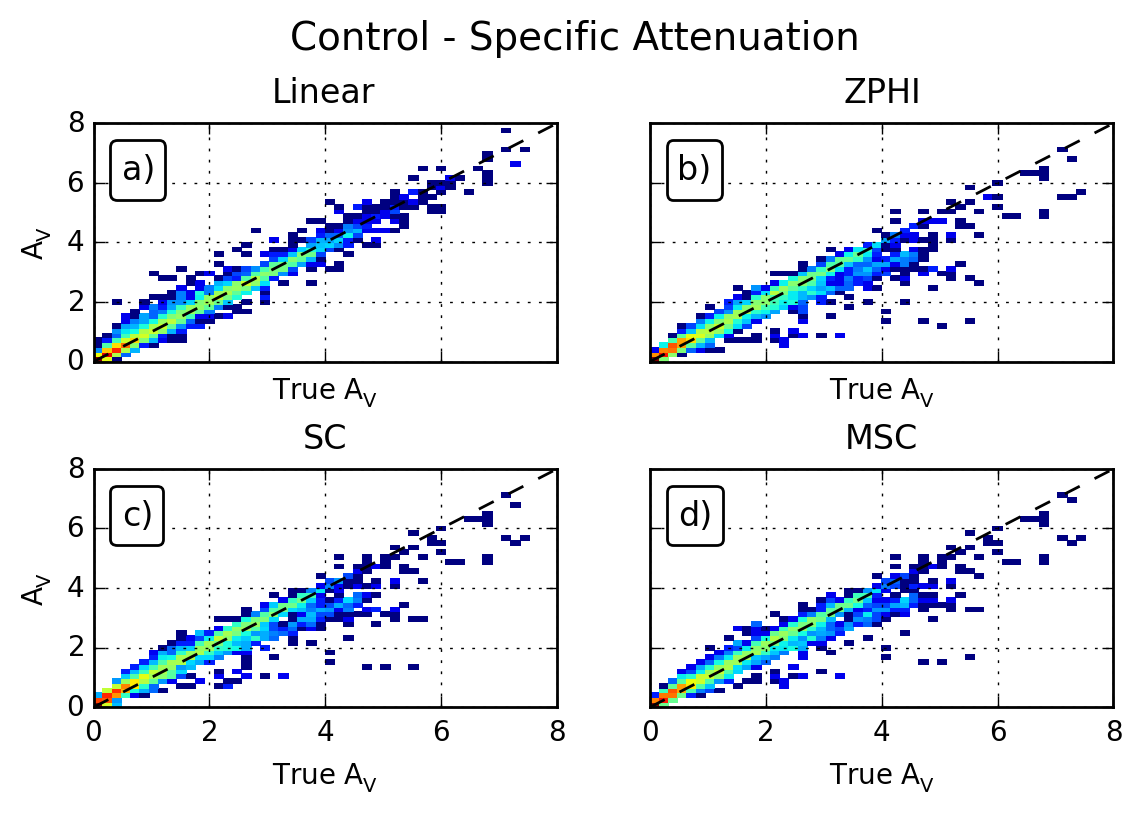
\includegraphics[scale=0.7]{figures/spatial/X_Control_Specific_Attenuation_V_scatter}
    \end{center}
\end{frame}

\begin{frame}
    \begin{center}
        \includegraphics<1>[scale=0.7]{figures/spatial/C_Sidelobe_Attenuation_V}
        \includegraphics<2>[scale=0.7]{figures/spatial/C_Control_Attenuation_V}
    \end{center}
\end{frame}

\begin{frame}
    \begin{center}
        \includegraphics<1>[scale=0.7]{figures/spatial/C_Sidelobe_Attenuation_Difference_V}
        \includegraphics<2>[scale=0.7]{figures/spatial/C_Control_Attenuation_Difference_V}
    \end{center}
\end{frame}

\begin{frame}
    \begin{center}
        \includegraphics<1>[scale=0.7]{figures/spatial/C_Sidelobe_Specific_Attenuation_V_scatter}
        \includegraphics<2>[scale=0.7]{figures/spatial/C_Control_Specific_Attenuation_V_scatter}
    \end{center}
\end{frame}

\begin{frame}
    \begin{center}
        \includegraphics<1>[scale=0.7]{figures/spatial/X_Sidelobe_Attenuation_V}
        \includegraphics<2>[scale=0.7]{figures/spatial/X_Control_Attenuation_V}
    \end{center}
\end{frame}

\begin{frame}
    \begin{center}
        \includegraphics<1>[scale=0.7]{figures/spatial/X_Sidelobe_Attenuation_Difference_V}
        \includegraphics<2>[scale=0.7]{figures/spatial/X_Control_Attenuation_Difference_V}
    \end{center}
\end{frame}

\begin{frame}
    \begin{center}
        \includegraphics<1>[scale=0.7]{figures/spatial/X_Sidelobe_Specific_Attenuation_V_scatter}
        \includegraphics<2>[scale=0.7]{figures/spatial/X_Control_Specific_Attenuation_V_scatter}
    \end{center}
\end{frame}

\begin{frame}
    \begin{center}
        \includegraphics<1>[scale=0.7]{figures/spatial/C_Beamwidth_Attenuation_V}
        \includegraphics<2>[scale=0.7]{figures/spatial/C_Control_Attenuation_V}
    \end{center}
\end{frame}

\begin{frame}
    \begin{center}
        \includegraphics<1>[scale=0.7]{figures/spatial/C_Beamwidth_Attenuation_Difference_V}
        \includegraphics<2>[scale=0.7]{figures/spatial/C_Control_Attenuation_Difference_V}
    \end{center}
\end{frame}

\begin{frame}
    \begin{center}
        \includegraphics<1>[scale=0.7]{figures/spatial/C_Beamwidth_Specific_Attenuation_V_scatter}
        \includegraphics<2>[scale=0.7]{figures/spatial/C_Control_Specific_Attenuation_V_scatter}
    \end{center}
\end{frame}

\begin{frame}
    \begin{center}
        \includegraphics<1>[scale=0.7]{figures/spatial/X_Beamwidth_Attenuation_V}
        \includegraphics<2>[scale=0.7]{figures/spatial/X_Control_Attenuation_V}
    \end{center}
\end{frame}

\begin{frame}
    \begin{center}
        \includegraphics<1>[scale=0.7]{figures/spatial/X_Beamwidth_Attenuation_Difference_V}
        \includegraphics<2>[scale=0.7]{figures/spatial/X_Control_Attenuation_Difference_V}
    \end{center}
\end{frame}

\begin{frame}
    \begin{center}
        \includegraphics<1>[scale=0.7]{figures/spatial/X_Beamwidth_Specific_Attenuation_V_scatter}
        \includegraphics<2>[scale=0.7]{figures/spatial/X_Control_Specific_Attenuation_V_scatter}
    \end{center}
\end{frame}

\begin{frame}
    \begin{center}
        \includegraphics<1>[scale=0.7]{figures/spatial/C_RadialWidth_Attenuation_V}
        \includegraphics<2>[scale=0.7]{figures/spatial/C_Control_Attenuation_V}
    \end{center}
\end{frame}

\begin{frame}
    \begin{center}
        \includegraphics<1>[scale=0.7]{figures/spatial/C_RadialWidth_Attenuation_Difference_V}
        \includegraphics<2>[scale=0.7]{figures/spatial/C_Control_Attenuation_Difference_V}
    \end{center}
\end{frame}

\begin{frame}
    \begin{center}
        \includegraphics<1>[scale=0.7]{figures/spatial/C_RadialWidth_Specific_Attenuation_V_scatter}
        \includegraphics<2>[scale=0.7]{figures/spatial/C_Control_Specific_Attenuation_V_scatter}
    \end{center}
\end{frame}

\begin{frame}
    \begin{center}
        \includegraphics<1>[scale=0.7]{figures/spatial/X_RadialWidth_Attenuation_V}
        \includegraphics<2>[scale=0.7]{figures/spatial/X_Control_Attenuation_V}
    \end{center}
\end{frame}

\begin{frame}
    \begin{center}
        \includegraphics<1>[scale=0.7]{figures/spatial/X_RadialWidth_Attenuation_Difference_V}
        \includegraphics<2>[scale=0.7]{figures/spatial/X_Control_Attenuation_Difference_V}
    \end{center}
\end{frame}

\begin{frame}
    \begin{center}
        \includegraphics<1>[scale=0.7]{figures/spatial/X_RadialWidth_Specific_Attenuation_V_scatter}
        \includegraphics<2>[scale=0.7]{figures/spatial/X_Control_Specific_Attenuation_V_scatter}
    \end{center}
\end{frame}

\begin{frame}
    \begin{center}
        \includegraphics<1>[scale=0.7]{figures/spatial/C_RangeResolution_Attenuation_V}
        \includegraphics<2>[scale=0.7]{figures/spatial/C_Control_Attenuation_V}
    \end{center}
\end{frame}

\begin{frame}
    \begin{center}
        \includegraphics<1>[scale=0.7]{figures/spatial/C_RangeResolution_Attenuation_Difference_V}
        \includegraphics<2>[scale=0.7]{figures/spatial/C_Control_Attenuation_Difference_V}
    \end{center}
\end{frame}

\begin{frame}
    \begin{center}
        \includegraphics<1>[scale=0.7]{figures/spatial/C_RangeResolution_Specific_Attenuation_V_scatter}
        \includegraphics<2>[scale=0.7]{figures/spatial/C_Control_Specific_Attenuation_V_scatter}
    \end{center}
\end{frame}

\begin{frame}
    \begin{center}
        \includegraphics<1>[scale=0.7]{figures/spatial/X_RangeResolution_Attenuation_V}
        \includegraphics<2>[scale=0.7]{figures/spatial/X_Control_Attenuation_V}
    \end{center}
\end{frame}

\begin{frame}
    \begin{center}
        \includegraphics<1>[scale=0.7]{figures/spatial/X_RangeResolution_Attenuation_Difference_V}
        \includegraphics<2>[scale=0.7]{figures/spatial/X_Control_Attenuation_Difference_V}
    \end{center}
\end{frame}

\begin{frame}
    \begin{center}
        \includegraphics<1>[scale=0.7]{figures/spatial/X_RangeResolution_Specific_Attenuation_V_scatter}
        \includegraphics<2>[scale=0.7]{figures/spatial/X_Control_Specific_Attenuation_V_scatter}
    \end{center}
\end{frame}

\begin{frame}
    \begin{center}
        \includegraphics<1>[scale=0.7]{figures/spatial/C_Combined_Attenuation_V}
        \includegraphics<2>[scale=0.7]{figures/spatial/C_Control_Attenuation_V}
    \end{center}
\end{frame}

\begin{frame}
    \begin{center}
        \includegraphics<1>[scale=0.7]{figures/spatial/C_Combined_Attenuation_Difference_V}
        \includegraphics<2>[scale=0.7]{figures/spatial/C_Control_Attenuation_Difference_V}
    \end{center}
\end{frame}

\begin{frame}
    \begin{center}
        \includegraphics<1>[scale=0.7]{figures/spatial/C_Combined_Specific_Attenuation_V_scatter}
        \includegraphics<2>[scale=0.7]{figures/spatial/C_Control_Specific_Attenuation_V_scatter}
    \end{center}
\end{frame}

\begin{frame}
    \begin{center}
        \includegraphics<1>[scale=0.7]{figures/spatial/X_Combined_Attenuation_V}
        \includegraphics<2>[scale=0.7]{figures/spatial/X_Control_Attenuation_V}
    \end{center}
\end{frame}

\begin{frame}
    \begin{center}
        \includegraphics<1>[scale=0.7]{figures/spatial/X_Combined_Attenuation_Difference_V}
        \includegraphics<2>[scale=0.7]{figures/spatial/X_Control_Attenuation_Difference_V}
    \end{center}
\end{frame}

\begin{frame}
    \begin{center}
        \includegraphics<1>[scale=0.7]{figures/spatial/X_Combined_Specific_Attenuation_V_scatter}
        \includegraphics<2>[scale=0.7]{figures/spatial/X_Control_Specific_Attenuation_V_scatter}
    \end{center}
\end{frame}

\end{document}